%%%%%%%%%%%%%%%%%%%%%%%%%%%%%%%%%%%%%%%%%
% Thin Sectioned Essay
% LaTeX Template
% Version 1.0 (3/8/13)
%
% This template has been downloaded from:
% http://www.LaTeXTemplates.com
%
% Original Author:
% Nicolas Diaz (nsdiaz@uc.cl) with extensive modifications by:
% Vel (vel@latextemplates.com)
%
% License:
% CC BY-NC-SA 3.0 (http://creativecommons.org/licenses/by-nc-sa/3.0/)
%
%%%%%%%%%%%%%%%%%%%%%%%%%%%%%%%%%%%%%%%%%

%----------------------------------------------------------------------------------------
%	PACKAGES AND OTHER DOCUMENT CONFIGURATIONS
%----------------------------------------------------------------------------------------
% oli: report
\documentclass[a5paper, 8pt, twocolumn]{book} % Font size (can be 10pt, 11pt or 12pt) and paper size (remove a4paper for US letter paper)
\usepackage[a5paper, margin=0.5in, top=0.75in]{geometry}
\usepackage[finnish]{babel}
\usepackage[utf8]{inputenc}
\usepackage{multicol}
\usepackage{icomma}
\usepackage{graphicx}
\usepackage{pdfpages}
\usepackage{graphics}
\usepackage{lipsum}
\usepackage{epstopdf}
\usepackage{nextpage}
\usepackage{amsmath}
\usepackage[protrusion=true,expansion=true]{microtype} % Better typography
\usepackage{graphicx} % Required for including pictures
\usepackage{wrapfig} % Allows in-line images
\usepackage{wasysym}
%\usepackage{showframe}
\usepackage{upgreek}
\usepackage{subfiles}
\usepackage{dblfloatfix}
\usepackage{makecell}
\usepackage[hyphens]{url}
\usepackage{cancel}
\usepackage{textcomp}
\usepackage[toc,page]{appendix}
\usepackage[style=authoryear,sorting=none,natbib=true,doi=true]{biblatex}
\usepackage{sectsty}
\usepackage{eurosym}
\let\quarternote\undefined
\let\eighthnote\undefined
\usepackage{arev}
\usepackage{placeins}
\usepackage{titleps}
\usepackage[tikz]{bclogo}
\usepackage{tabularx}
%\addbibresource{sample2.bib}
\usepackage{mathpazo} % Use the Palatino font
\usepackage[T1,T5]{fontenc} % Required for accented characters
\usepackage[hypcap,font=singlespacing]{caption}
\linespread{1.0} % Change line spacing here, Palatino benefits from a slight increase by default
\usepackage{hyperref}
\hypersetup{colorlinks=true,citecolor=black}
\numberwithin{equation}{section}

%\epstopdfsetup{outdir=./images}

\setlength{\parindent}{1em}
\setlength{\parskip}{0.5em}
\subsectionfont{\raggedright}
\subsubsectionfont{\raggedright}
\newpagestyle{ruled}
{\sethead{\chaptertitle}{}{\scalebox{0.5}{
\includegraphics{limes_logo1cm.eps}}}\headrule
	\setfoot*{}{}{\usepage}}
\pagestyle{ruled}

\graphicspath{{images/}{../images/}}

\makeatletter
\renewcommand{\bibfont}{\normalfont\small}
\renewcommand\@biblabel[1]{\textbf{#1.}} % Change the square brackets for each bibliography item from '[1]' to '1.'
\renewcommand{\@listI}{\itemsep=0pt} % Reduce the space between items in the itemize and enumerate environments and the bibliography

\hyphenation{LiEKe}
%----------------------------------------------------------------------------------------
%	TITLE
%----------------------------------------------------------------------------------------
\title{Älä hätäile}
\date{2019}
\author{Limes ry}
\begin{document}
\raggedbottom
\frontmatter
\null
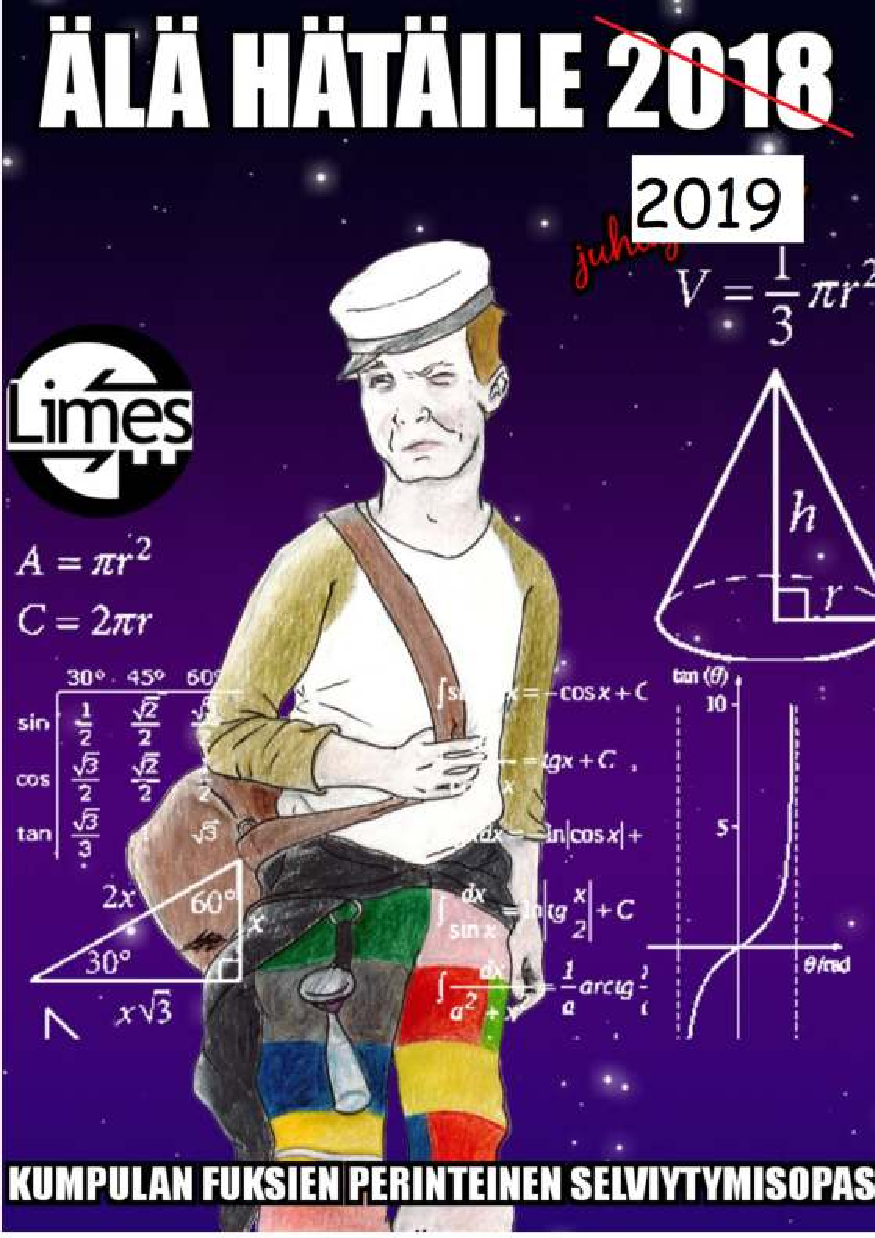
\includepdf[pages={-},angle=0]{ahiskansilehti.pdf}

\thispagestyle{empty}
\begin{figure*}[h!]
	\href{https://www.facebook.com/events/495938574557920/}{\includegraphics*[width=\textwidth]{tiedebasaari.jpg}}
\end{figure*}
\begin{figure*}[h!]
	\href{https://www.facebook.com/events/613237405833437/}{\includegraphics*[width=\textwidth]{fuksidisko.jpg}}
\end{figure*}
\begin{titlepage}
	\begin{center}
		\vspace*{1cm}
		
		\Huge \textbf{Älä hätäile}
		
		\vspace{0.5cm}
		\Large 2019
		
		\vspace{1.5cm}
		
		\Large \textbf{Limes ry}
		
		\vfill

		\vspace{0.6cm}
		
		
\includegraphics[width=0.4\textwidth]{einstein.png}
		
		HELSINKI 2019
	\end{center}
\end{titlepage}
\noindent%\begin{table}[!t]
	\begin{tabularx}{\textwidth}{@{}llll}
	\textbf{Julkaisija} & Limes ry & \textbf{Kannet} & Markus Riskumäki\\
	\textbf{Päätoimittaja} & Sakari Väkevä & \textbf{Painos} & -- \\
	\textbf{Toimituskunta} & Lauri Franzon & \textbf{Painatus} & -- \\
	& Matias Jääskeläinen & \textbf{ISBN} & -- \\
    & Laura Kaurijoki & & -- \\ & Auli Salmi & &
\end{tabularx}
%\end{table}

\noindent\fbox{\begin{minipage}{\textwidth}
\centering {\bfseries Ähikseen kirjoittaneet kautta aikain (vuosina 1991--2018) }
\tiny\begin{multicols}{5}
{\begingroup \obeylines 
\input{tekijat.txt} \endgroup}\end{multicols}\end{minipage}}

%----------------------------------------------------------------------------------------
\begingroup
\makeatletter
% Redefine the \chapter* header macro to remove vertical space
\def\@makeschapterhead#1{%
	%\vspace*{50\p@}% Remove the vertical space
	{\parindent \z@ \raggedright
		\normalfont
		\interlinepenalty\@M
		\Huge \bfseries  #1\par\nobreak
		\vskip 40\p@
}}
\makeatother
\setcounter{secnumdepth}{0}
\setcounter{tocdepth}{1}

\tableofcontents
\endgroup

%----------------------------------------------------------------------------------------
%	ESSAY BODY
%----------------------------------------------------------------------------------------
\emergencystretch 3em
\chapter{Johdanto}
\twocolumn[\section{Oppaasta}]
Käsissäsi on tukeva paketti perimä\-tietoa opiskelusta ja opiskelija\-elämästä keisarillisessa Aleksanterin Yliopistossa. Vanhempien opiskelijoiden suulla Älä Hätäile kertoo sinulle (opiskelija)elämästä, maailmankaikkeudesta ja muusta sellaisesta, joka on hyödyllistä ja välttämätöntäkin tietää, mutta jonka usein oppii vasta kantapään kautta. Tavoitteena on opastaa sinut läpi opiskelun alkumetrien karikoiden tutustumaan avarakatseisesti ja ennakkoluulottomasti opinahjoosi, yliopistoyhteisöön ja kaikkiin sen pikku merkillisyyksiin. 

Toinen tärkeä tavoitteemme on tehdä tästä oppaasta nimensä veroinen ``vaihtoehtoinen opinto-opas'' ja tarjota vaihtoehtoja sille opetussuunnitelmalle, jota yliopisto virallisesti esittää. Lisäksi haluamme johdattaa sinut alkuun yliopiston tietotekniikkajärjestelmien käytössä. 

Kirjan ensimmäisessä osassa opiskelijat kertovat löydöistään ja tunnelmistaan yli\-opisto\-kaupungissamme. Löydät siitä vinkkejä opiskelu\-ympäristöstäsi täydellä teholla nauttimiseen. Mukana ovat myös kampusten kartat tärkeine osoitteineen. Toinen osa kertoo laajasti opiskelusta, paitsi yleisestä näkökulmasta, myös yksityis\-kohtaisesti kaikkien ML-tieteen\-alojen eris\-kummallisuuksista ja pikku\-nikseistä. 

Niin ikään uudet päivähoitopaikkasi -- koulutus\-ohjelmat -- ja niiden virikkeelliset kurssit tulevat tutuiksi, niiden mystiset lyhenteet selkenevät, ja opintojesi suunnittelu toivottavasti helpottuu. Kolmannessa osassa kerromme myös vaihtoehtoisista oppikirjoista, joita voi lukea kurssikirjojen ohella tai omaksi iloksi. 

Neljännessä osassa esittäytyvät eksaktille luonnontieteilijälle tärkeimmät opiskelijajärjestöt ja muut tärkeät yhteydet yliopistolla. Opiskelijajärjestöihin tutustuminen ja niiden toimintaan osallistuminen lisäävät huomattavasti
sinunkin mahdollisuuksiasi viihtyä
yliopistolla ja myös itse vaikuttaa opiskeluolosuhteisiisi.

Kirjan viidennessä osassa raapaistaan
kyberavaruutta tutustumalla lyhyesti
yliopistolla tarjolla oleviin tieto\-järjestelmiin
ja miten niitä pääsee käyttämään.
Viimeinen, muttei vähäpätöisin osa opasta
on Opiskelijan sanasto. Käsittämättömien
lyhenteiden ja mielikuvituksellisen opiskelijaslangin
sekametelisoppa on omiaan sekoittamaan
uuden opiskelijan pään. Älä Hätäile,
sillä viralliset ja epäviralliset termit, paikat ja
ilmiöt saavat selityksensä tässä Kaiken Äässä
ja Öössä.

Älä Hätäile on muotoutunut lukuisien
opiskelijasukupolvien kirjoittamana; osa
oppaan ajattomista teksteistä periytyy aina
muinaisen 80-luvun puolivälistä asti, osa on
uunituoretta, vasta itsekin hiljattain aloittaneiden
opiskelijoiden kirjoittamaa. 

Kiitokset
kuuluvat kaikille niille lukemattomille, jotka
ovat uhranneet hikipisaransa ja yöunensa
tämän oppaan ja sen edeltäjien eteen. Moni
heistä on jo valmistunut yliopistolta tai muuten
kypsynyt, mutta heidän kirjoituksensa
elävät edelleen apuna uusille. Kiitoksia myös
kuvamateriaalista, jota olemme omin luvin
tai luvatta häikäilemättä lainanneet niin epämääräisistä
kuin määräisistäkin lähteistä.

Me kaikki toivomme, että opiskeluaikanasi
olet yksi meistä aktiivisista opiskelijoista
ja että opintojesi päätyttyä voit sanoa
opiskeluaikasi olleen elämäsi parasta aikaa!

\vspace{0.5cm}
\noindent\textsc{Toimitus}

\twocolumn[\section{Älä Hätäilen historia} {\small \itshape ``Ähiksen lyhyt historia''}\vspace{0.5cm} ]
Tämä katsaus Älä Hätäilen, tuttavallisemmin
Ähiksen, historiaan on lyhyt vilkaisu
opinto-oppaan taustoihin, mutta ei
suinkaan ole tieteellinen tutkimus tai historiikki.
Lähteinä ovat olleet Limeksen hallitusten
pöytäkirjat, Sykloidit, perimätieto ja
erityisesti Aku Valtakosken ja Sami ``Niksu''
Nikanderin artikkeli ``Instituutio nimeltä
Älä Hätäile'' JuhlaKissoidi-lehdestä
vuodelta~2001.

\begin{figure*}[!b]
	\centering
	
\includegraphics[width=0.6\textwidth]{dontpanik1.png}
\end{figure*}
Älä Hätäilen historia ulottuu kauemmas
kuin voisi nimestä päätellä. Nimi on
peräisin Douglas Adamsin vuonna~1978
BBC:ssä ensiesitetystä kuunnelmasta
Linnunradan käsikirja liftareille (The
Hitchhiker's Guide to the Galaxy). Opinto-oppaan
juuret ovat kirjallisissa opinto-ohjeissa,
jotka ensimmäisen kerran painettiin
vuonna~1955 Limeksen silloiseen lehteen,
Kissoidiin. Vuosina~1959 ja 1960 ilmestyivät
pelkästään opinto-ohjausta sisältäneet
erikoisnumerot, Opas-Kissoidit. Limeksen
opintoneuvojien ohjeita painettiin Kissoideihin
vuoteen~1966 asti, jolloin ohjeista
koottiin ensimmäinen varsinainen Limeksen
opinto-opas. Kesti vuosikausia ennen
kuin yliopisto alkoi julkaista virallisia
opinto-oppaita. Limeksen ensimmäisestä
opinto-oppaasta säilyi Älä Hätäilessä ainakin
vuoteen~2000 asti Helsingin keskustan
kartta ja laitosten pohja\-piirroksia.

Limeksen opinto-opasta painettiin ilman
erityistä nimeä vuoteen~1969 asti. Vuonna
1970 ilmestyi vasemmistolaisen opiskelija\-radikalismin
seurauksena Limeksen Myyopas,
jonka tekijänä oli Lietso eli Limeksen ASS-siipi. Virallisesti Limes~ry irti\-sanoutui
Akateemisen Sosialistiseuran teettämästä
Myyoppaasta. Vaikutuksensa tällä uudella
kriittisen asenteen omaavalla opinto-oppaalla
kuitenkin oli, sillä siinä ensimmäistä
kertaa käsiteltiin opiskelijoiden sosiaali\-poliittisia
asioita kuten tulot ja asuminen sekä
esiteltiin muita opiskelija\-järjestöjä. Nämä
aiheet ovat säilyneet nykyisen Älä Hätäilen
sisällössä.

Vuosina 1971--1973 ilmestyi Opiskelijan
rautaisannos. Se ei ollut pelkästään Limeksen
opinto-opas, sillä se tehtiin yhdessä
ANK:n (Ainejärjestöjen Neuvottelukunta)
kanssa. Rautaisannos oli sisällöllisesti yhtä
lailla poliittisesti punaiseksi värittynyt,
kuten oli ollut Myyopaskin. Vuonna~1975
Limes ei varsinaisesti tehnyt omaa opinto-opasta,
vaan tilalle tarjottiin ANK:n Uusi
opiskelija "-opasta. Limeksessä palattiin
vuosiksi~1976--1981 aikaisempaan tapaan
eli opinto-oppaan sijasta opintoneuvoja
julkaistiin Limeksen uudessa Sykloidilehdessä.
Limeksen vuonna~1964 perustettu
kaksisivuinen tiedotuslehti Sykloidi oli
1970-luvulla ottanut aiemman Limeksen
lehden, Kissoidin, tehtävän kokonaisuudessaan.
Kissoidi muuttui sittemmin vain
viiden vuoden välein ilmestyväksi Sykloidin
erikoisnumeroksi ja vuosijuhlajulkaisuksi,
JuhlaKissoidiksi.

Vuonna~1982 Limes~ry ja HYK (Helsingin
Yliopiston Kemistit) tekivät yhdessä
opinto-oppaan nimeltään Verta, Hikeä ja
Kyyneleitä eli VHK. Voimakkain poliittisuus
sisällössä oli jo mennyttä. Kirjasta ilmestyi seuraavana vuonna päivitetty versio.
Limes julkaisi vuonna~1984 VHK:sta
päivitetyn version nimellä Hellyydellä
uusille. Vuonna~1985 nimi muuttui MFK-kirjaksi.
VHK seuraajineen oli siten malli
nykytyylille, jossa päivitetään vanhaa
opasta. Näistä kirjoista on saattanut säilyä
ja siirtyä osa teksti\-sisällöstä nykyiseen Älä
Hätäileen. MFK-kirjassa uutuutena olivat
sivuaine-esittelyt muista tiede\-kunnista,
opiskelijan sanasto ja ruokala-arvostelut.

Vuonna~1987 ilmestyi ensimmäinen Älä
Hätäile, josta alkaen kirjan nimi on pysynyt
samana kansikuvan vaihtuessa vuosittain
ja sisällön päivittyessä. Älä Hätäile voitti
vuonna~2006 HYYn opinto-oppaiden kilpailun.
Voittoa himmentää se, että ensimmäinen
sija jaettiin kolmen opinto-oppaan
kesken. Vastineeksi hupia tuottaa se, että
Ä:n pisteet unohtuivat HYYltä kunnia\-kirjasta,
johon on kirjoitettu ``Alä Hätäile''.
Käykäähän katsomassa Limeksen toimistolla
kunniakirjaa. Jollei sitä ole enää seinällä,
niin käskekää laittamaan, sillä teos ja
tekijät ovat kunniakirjansa ansainneet.

Vuodesta~2017 lähtien yliopiston viralliset opetussuunnitelmat ovat saatavilla vain nippuna Wiki-taulukoita ja kokoelmana mystisiä valintasääntöjä, eikä paperista opinto-opasta enää julkaista. Siksi Limeksen opinto-oppaalla on edelleen tilauksensa uusille opiskelijoille
toimivana tieto\-lähteenä. 

\vspace{0.5cm}
\noindent\textsc{Ilmo Teikari}\\
\noindent\textsc{Sakari Väkevä}

\twocolumn[\section{Pallo hukassa} {\small \itshape ``\dots eli otteita aloittelevan opiskelijan muistelmista.''}\vspace{0.5cm}]
Aina pitää olla kiire, miksen olisi voinut
lähteä ajoissa? Kiireesti maksamaan
laskuja, opinto\-toimisto sulkee kohta ja
HYYn jäsenmaksu ja terveyden\-hoito\-maksu
pitää olla maksettuna\dots juoksen opinto\-toimistoon
-- mitä, eikö se suljekaan vielä
kolmeen tuntiin? No, ottakaa nyt nämä
ilmoit\-tautumis\-kaavakkeet
vastaan\dots ai kaavake
1002.1B puuttuu, hmm\dots tuossahan
se on, olkaa hyvä, kiitos -- saan leiman
pankki\-siirto\-kuittiin.

Tällaisten seurassako minä vietän seuraavat
keski\-määräiset 6,5~vuotta? Vajaan
tuhannen ihmisen luentosali puolillaan ihmisiä,
tunnelma on painostava, kukaan ei
uskalla taputtaa dekaanin puheelle -- olisikohan
Dante saanut innoituksensa tällaisessa
ilmapiirissä? Vaipuisin masennuksen
valtaan, ellen tuntisi salin kidutus\-penkkien
asukkaista ketään -- tyydyn kuitenkin
vain haukotukseen: opintoneuvoja, HYYn
edustaja ja Kielikeskuksen muorit heittävät
lusikkansa soppaan ja hämmentävät
särkevää päätäni. Löytyykö keltään punaista
lankaa?

Kolmannen info\-istunnon lopulla alkaa
selvitä, että meidän pitää laatia luku\-järjestys
-- sen selville saaminen ei aivan
vienyt yhdeksää tuntia. Opinto\-neuvoja on
hukkua kysymyksiin -- aivan, jotkut uskaltavat
kysyä! Yliopisto on edelleen hämärä
käsite, mutta pimeys ei ole enää yhtä
täydellinen. Päätös\-sanat saavat viimeinkin
aikaan ne kauan kaivatut aplodit, ehkä täällä
sittenkin voi viihtyä.

\begin{figure}
	\centering
	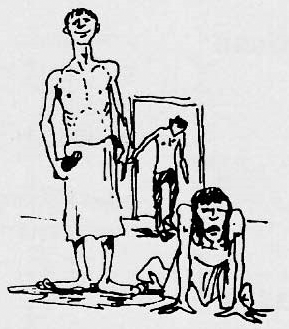
\includegraphics[width=0.8\columnwidth]{pallohukassa1.png}
\end{figure}
Tarjoa tuutorillesi kalja, sanotaan\dots Tarkoittakohan se sitä, että kaikkien tuutoroitavien pitäisi tehdä se samana iltana?
Voi tuutori\-parkaa.

Limes järjestää sauna\-illan uusille opiskelijoille.
Mikäs siinä, kyllä sauna kelpaa.
Täällähän on melkein täyttä\dots Moi, sut mä
oon nähny luennoilla\dots ai, sulla tulee sen
verran opintopisteitä\dots Saunaan, uimaan,
makkaraakin vois paistaa -- pahus, viimeinen
bussi lähtis kohta, nyt tarttis lähtee\dots
äh, no menköön. Hei, sähän oot Limeksen
hallituksessa, kerros mitä te oikein teette
-- hei, toihan vois olla hauskaa,
mä tuun seuraavaan kokoukseen kattomaan. Varjo\-puolensa
kaikella: herään
siihen, että joku
yrittää yrjötä päälleni.
Huti.

Ankaran meditoinnin tulos: maksan kaksitoista euroa ja liityn osakuntaan.
Enhän minä tunne täältä ketään. Minkäslaista
väkeä täällä on paikalla? Löytyy
matemaatikkoja, tietojen\-käsittelijöitä ja
muita terveitä ihmisiä. Sitten on muutamia
humanisteja ja valtio\-tieteilijöitäkin, melko vaarattoman näköisiä kyllä. Noistako niitä
terroristeja ja poliitikkoja tulee, hmm\dots
Otetaanpa selville: anteeksi, mikä sinusta
tulee isona? Mielenkiintoista, kukaan
ei tunnu tietävän. Hei tuolla on jopa yksi
teekkari! Pitäisiköhän lähteä karkuun ennen
kuin se puree.

Saamaton täytyy opiskelijan olla, jos
tulee tekemisestä puute. Tee kuten minä,
selaa yo-kalenterin järjestöt läpi ja rasti
kiinnostavan tuntuiset tai seuraa Ylkkärin (tulee jokaiselle kotiin aikanaan) tapahtumailmoituksia. Aika tulee pian tarkkaan
käytettyä, sano.

Välikoe lähestyy, opiskellakin pitäisi.
50~sivua puolessa tunnissa, onko tässä mitään
tolkkua? Ei tänne romaaneja tultu lukemaan.
Viime viikon laskareihinkin meni
kymmenen tuntia, olenko huono? Kyllä
tämä tästä, muut ovat melkein yhtä huonoja.
Melu kirjastossa huumaa, kahvilassakin
olisi hiljaisempaa -- voikohan teetä juoda
liikaa?
\begin{figure}
	\centering
	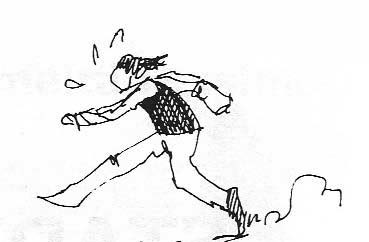
\includegraphics[width=0.8\columnwidth]{pallohukassa2.png}
\end{figure}

Huh, huh, pitää rentoutua välillä, lihaksetkin
alkavat rapistua liiasta työnteosta.
Yliopisto\-liikunta tarjoaa kaikenlaista koriksesta
ja sählystä budolajeihin ja tansseihin,
mikähän sopisi minulle? Suunnistus,
miksei, uintikin olisi halpaa. Kulttuuri\-nälkä
heräsi. Limeksen elokuva\-kerho,
Vanha, Ylioppilas\-teatteri, Elokuva-arkisto\dots en ole
vielä ehtinyt kyllästyä Hesan kulttuuri\-elämään.

Syyslukukauden viimeiset kokeet olivat
ja menivät. Mitä tänä syksynä opimme?
Emme jälleen mitään. Mutta muista, että
kaikista tenteistä pääsee läpi ennen valmistumistaan!

\setlength{\fboxsep}{5pt}
\setlength{\fboxrule}{2pt}
\noindent\begin{figure*}\makebox[\textwidth][c]{\fbox{\begin{minipage}{\textwidth}
Yliopiston loppukoe 13.5. Kirjoita paperiin OMA nimesi ja henkilö\-tunnus.

\begin{enumerate}
	\item Yliopistoon pyrkivien vuosittainen määrä olkoon $n$. Näistä $a$ suorittaa
	tutkintonsa viidessä vuodessa ja $b$ joskus. Laske valmistuvien filosofian
	magisterien lukumäärä vuotta kohden. Voit olettaa, että $b$ on pieni ja $a/n\sim0$.
	\item Johda.
	\item Olkoon väittämä: Jos tiedät, että et tiedä tietäväsi tietämättömyyttäsi,
	tieten tahtoen tietoisuutesi tien, tietänet tietäväsi. Määritä lauseen syntaktinen
	ja semanttinen rakenne ja tee metasympaattinen Jaawa-ohjelma, joka toimii.
	\item Lorenz-muunnoksen merkillisyys. Arvioi tämän perusteella
	todennäköisyys, mihin tämä maailma on menossa.
\end{enumerate}

Tulokset pian. Uusintakokeeseen ilmoittaudutaan.
Valitustilaisuus on. \\Malliratkaisuja tulee.
\end{minipage}}}\end{figure*}
\mainmatter
\chapter{Stadissa}
\subfile{sections/stadissa}

\chapter{Opintiellä}
\begin{figure*}
	\centering
	
\includegraphics[width=0.8\textwidth]{hypaarakennus.png}
\end{figure*}

\twocolumn[\section{Opintotuki ja turva} {\small \itshape ``Vielä 90-luvun puolivälissä opiskelija saattoi harjoittaa akateemista vapautta mielensä mukaan; opintotuki tuli tilille joka kuukausi opintojen edistymisestä riippumatta. Nyttemmin on myös ylioppilaisiin alettu soveltaa tulosvastuuperiaatetta, mikä merkitsee rahan tulon loppumista, mikäli opinnot eivät edisty.''}\vspace{0.5cm}]
Nykyinen Kelan vaatima opinto\-piste\-määrä
on viisi tutkintoon kuuluvaa opinto\-pistettä
tuki\-kuukautta kohden. Vuodessa
pitäisi siis opiskella vähintään 45~op, ei mikään
pieni määrä. Lisäksi opinto\-tukea nostavan
opiskelijan tulee saada vähintään 20~opinto\-pistettä lukuvuotta kohden, riippumatta
nostettujen tukikuukausien määrästä.
Jos aikoo valmistua viidessä vuodessa, on tavoitetaso vielä tiukempi -- noin 60~op per lukuvuosi.

Alempaa korkeakoulututkintoa
varten myönnetään aluksi
30~tukikuukautta, ja vasta sen suorittamisen
jälkeen saa lisää tukikuukausia ylempää
korkeakoulututkintoa varten, maksimissaan
21~tukikuukautta. Yhteensä tukikuukausia
ei kuitenkaan saa yli 48:aa, joten alemmassa
tutkinnossa ylimääräiset käyttämäsi
tukikuukaudet vähentävät ylempään tutkintoon
jääviä. On siis syytä keskittyä myös
opiskeluun ensimmäisestä lukuvuodesta
lähtien, vaikka järjestö- ym.\,toiminta veisikin
mukanaan. Tukikuukausien enimmäismäärä
on suhteellisen pieni, ei siis olekaan
mikään ihme, että ``täysipäiväisestä'' järjestöhörhöilystä
kiinnostuneiden määrä on
ollut laskemaan päin. Sääli.

Jos kuitenkin käy niin, etteivät opintosi
suju suunnitelmien mukaan, ei hätä ole
tämän näköinen. Opintojen edistyminen
tarkistetaan syksyisin, ja tällöin lasketaan
koko edellisen lukuvuoden (alkaa 1.\,elokuuta
ja päättyy 31.\,heinäkuuta) opintopisteet.
Kesätenteissä on siis vielä mahdollisuus
korjata opintopistesaldoa. Mikäli tämä ei onnistu, Kela tarkastelee koko opintoaikana hankittua opintopistekertymää ja arvioi, ylittääkö se 5~op/tukikuukausi. Mikäli
määrä ei tämän jälkeenkään riitä Kelan tädeille,
lähettävät he selvityspyynnön opinnoista.
Tuen keskeyttämisen voi tässä
vaiheessa estää kaivamalla jostakin merkitsemättä
jääneitä opintosuorituksia (myös
järjestötoiminnasta saa opintopisteitä!).
Lisäksi ainakin periaatteessa tilanne katsotaan
tapauskohtaisesti, jolloin myös aikaisempien
vuosien opintomenestys voi vaikuttaa
puoltavasti tuen jatkumiseen -- sitä
tapahtuuko näin oikeasti voi vain arvailla.

Opintotuki muodostuu kahdesta osasta: opintorahasta ja opintolainan valtiontakauksesta. Opintoraha on se osa opintotuesta, jota ei tarvitse maksaa takaisin. Itsenäisesti asuva 18 vuotta täyttänyt voi saada sitä enintään 250,28~euroa kuussa. Opintoraha on veronalaista tuloa, mutta vuodesta~2019 alkaen Kela ei enää suorita siitä automaattisesti ennakonpidätystä. Jos sinulla on opintorahan lisäksi muita veronalaisia tuloja, opintoraha on huomioitava muiden tulojen ennakonpidätyksessä. Tarkista Verohallinnon sivuilta löytyvällä laskurilla, ylittääkö tulosi verokortin tulorajan. Voit halutessasi ilmoittaa Kelalle sopivan ennakonpidätysprosentin pidätettäväksi suoraan opintorahasta -- työssä käyvälle opiskelijalle tämä voikin olla järkevää.

Myönteisen opintotukipäätöksen antaessaan
Kela myöntää suoraan valtion takaaman opintolainan, joka
sitten nostetaan omasta pankista (ja on
myös maksettava takaisin!) Opintolainan
suuruus on 650~euroa tukikuukautta kohden.
Takaus kannattaa joka tapauksessa
hakea jo opintojen alussa, sillä se voidaan
myöntää aikaisintaan hakemiskuukauden
alusta lukien. Lainaa voi nostaa syksyllä aikaisintaan
1.8.\,ja keväällä 1.1. 

Nostamatta
jääneet lainaerät voi käyttää myöhemmin
saman lukuvuoden aikana -- ei kuitenkaan
opintotukiajan tai opintojen päättymisen
tai opintojen keskeyttämisen jälkeen. Lainaa
ei myöskään saa nostaa sen jälkeen,
kun opintotuki on lakkautettu puutteellisen
opintomenestyksen vuoksi. Kannattaa siis
todella pitää silmällä opintomenestystä. Jos suoritat tutkintosi määräajassa (6~lukuvuotta) ja sinulla on opintolainaa yli 2~500~euroa, Kela maksaa osan opintolainastasi opintolainahyvityksen muodossa.

Jos esim.\,sairauden vuoksi opintoja ei ole kertynyt riittävästi ja
tuki keskeytetään, Kelan päätöksessä ei välttämättä ole
kehotusta hakea sairauspäivärahaa. Tämän vuoksi kannattaa tiukassa tilanteessa aina kysyä neuvoja Kelan opiskelijoiden palvelunumerosta (020~692~209, ma--pe klo 8--17). Mikäli koet tulleesi kohdelluksi epäoikeudenmukaisesti, Kelan päätöksiin voi hakea muutosta. Jos Kelan mielestä päätöstä ei voi oikaista haluamallasi tavalla, valitus ohjataan opintotuen muutoksenhakulautakuntaan, ja valittamista voi jatkaa vakuutusoikeuteen saakka. 

Jotta tukiruletti menisi vieläkin monimutkaisemmaksi,
tarkkaillaan myös opiskelijan
muita tuloja. Saat tienata vapaasti
667~euroa tuellista ja 1~990~euroa tuetonta
kuukautta kohden. Tuloja tarkastellaan
koko kalenterivuoden ajalta. Mikäli tukea
on maksettu liikaa, peritään se korkoineen
takaisin. Ylitystä saa olla enintään
222~euroa. Tämän voi välttää maksamalla
jo myönnetyt tuet takaisin tai perumalla
opintotuen joiltakin kuukausilta. Kannattaa
siis suunnitella opintotuen ottaminen joka
vuosi ja säilyttää kaikki palkkakuitit, jotta
välttyy ikäviltä yllätyksiltä!

Erityisesti kannattaa tarkkailla vuodenvaihteen
palkkakuitteja, sillä mikäli palkka
tupsahtaa tilillesi 1.1.2019 eikä vaikkapa
31.12.2018 vaikuttaa se eri tulovuoteen.
Varoittavana esimerkkinä opiskelija, joka
palautti vapaaehtoisesti vuoden~2011 tukia,
ja vuoden~2012 tukia taasen perittiin häneltä
pois korkojen kera, koska palkka oli tullut
3.1.2012! Takaisin perityt tukikuukaudet
menetetään pysyvästi, vapaaehtoiset
kuukaudet taasen voi nostaa myöhemmin.
\footnote{Vinkki, jota emme sinulle anna, on nostaa
palkka pimeänä. Näin se ei vaikuta opintotukeen.
Nudge nudge.}

Yleistä asumistukea täytyy hakea erikseen, ja se maksetaan koko ruokakunnalle. Tämän vuoksi haluat ehkä varmistaa, että sinut ja kämppiksesi lasketaan eri ruokakuntiin. Tämä onnistuu esimerkiksi laatimalla erilliset vuokrasopimukset, joissa vuokralaiset eivät ole yhteisvastuussa koko asunnon vuokrasta. Kela saattaa kuitenkin epäillä tätä ja vaatia todistamaan, etteivät asuinkumppanit ole suhteessa keskenään, tai muuten toisen tulot vaikuttavat myös toisen saamaan asumistukeen. HYY on lobannut voimakkaasti tätä ``ruokakuntakohtaisuutta'' vastaan, mutta ainakaan syksyllä~2019 asumistuki ei ole vielä yksilökohtainen. Asumistuki on 80~\% hyväksyttävien asumismenojen ja perusomavastuun erotuksesta. Kaikkein pienituloisimmilla ei ole ollenkaan perusomavastuuta. 

Viimeisenä tukivaihtoehtona voi köyhä
opiskelija turvautua perus\-toimeen\-tulo\-tukeen, jota haetaan Kelalta.
Toimeentulotukea voi saada
vasta kun kaikki lukuvuoden opintoetuudet on käytetty,
myös opintolaina. Lisäksi opiskelijan tulee todistaa, ettei hän työnhausta huolimatta ole saanut töitä eikä voi kesällä suorittaa tutkintoaan edistäviä opintoja ja hakea niihin kesäajan opintotukea. Myös mahdolliset säästöt on käytettävä. Muutenkin ``sossun kassalle''
joutuminen voi olla mielenkiintoinen
tai vittumainen kokemus, riippuen elämänasenteesta.
Työttömyysturvaan opiskelija
ei ole oikeutettu kesällä, ellei luovu opiskelijan
statuksestaan syksyllä -- ja sen mukana
tulevista eduista.

\vspace{0.5cm}
\noindent\textsc{Aku Valtakoski}\\
\textsc{Anu Kontio}\\
\textsc{Ilmo Teikari}\\
\textsc{Risto Karinkanta}\\
\textsc{Riikka Saarelainen}\\
\textsc{Jani Kaipainen}\\
\textsc{Sakari Väkevä}

\twocolumn[\section{Miten suoritan tutkintoni?}]
Tutkintojen ja kurssien laajuudet määritellään
opintopisteinä. Virallinen määritelmä
kertoo, että 1600~tunnin työpanos
vastaa 60~opintopistettä. Taskulaskinta
käyttämällä huomaat, että yksi opintopiste
vastaa 26~tunnin ja 40~minuutin työtä. Totuus
voi joskus poiketa rajusti tästä, mutta
nyt kurssien laajuuksia on yritetty ihan oikeasti arvioida. Perustutkintorakenne
on kaksiportainen. Tiedekunnassa
suurin osa opiskelijoista saa samalla kertaa
suoritusoikeuden sekä alempaan että
ylempään tutkintoon. Alemman tutkinnon
tai sitä vastaavat opinnot muualla suorittaneille
voidaan myöntää pelkän ylemmän
tutkinnon suoritusoikeus. Alempi korkeakoulututkinto
on nimeltään luonnontieteen
kandidaatti (LuK) ja laajuudeltaan
180~opintopistettä. Ylempi tutkinto on filosofian
maisteri ja sen laajuus on (LuKin
jälkeen) 120~opintopistettä. Tutkintojen laajuudet saavat ylittyä enintään kymmenellä prosentilla, mutta enemmänkin saa ja ehkä jopa kannattaa opiskella -- tutkintoon sisältymättömät opinnot näkyvät kumminkin opinto\-suoritus\-otteella, jonka voi liittää esi\-merkiksi CV:n liitteeksi. FM-tutkinnon jälkeen voi jatkaa tieteellisiin jatkotutkintoihin, joista tunnetuin on filosofian tohtorin tutkinto.
\subsection*{Luonnontieteen kandidaatin tutkinto}
Ensimmäiseksi aloitetaan opiskelu kohti
luonnontieteen kandidaatin tutkintoa.
Tutkinnon virallinen tavoitesuoritusaika
on kolme vuotta, tosin luonnon\-tieteellisen alan
todellinen suoritus\-aika lienee joskus hieman pidempi.
Opintojen alkupuolella jokaiselle
opiskelijalle laaditaan henkilökohtainen
opintosuunnitelma (HOPS), jossa laaditaan
ohjaajan johdolla jonkinlainen suunnitelma
opintojen suorituksesta. Suunnitelmaa tarkistetaan
määräajoin ja siihen tehdään tarvittavat
korjaukset. Tarkoitus ei siis ole, että HOPS
olisi jonkinlainen pakkopaita, vaan pikemminkin
suuntaa antava kehys. Suunnitelmien
muoto vaihtelee koulutusohjelmasta toiseen
ja siihen pitäisi muotoilla suunnilleen,
mikä sinusta tulee isona. Muista kuitenkin:
Älä hätäile, vaikket vielä tietäisikään,
mitä haluat tehdä. Ensimmäisen vuoden opinnot
ovat melkein samat kaikille ja vuoden kuluttua
olet (toivottavasti) viisaampi.

Kandiohjelman opetussuunnitelmassa perusopintojen laajuus on vähintään 25~op, ja perus- ja aineopintojen laajuus on yhteensä vähintään 60~op. Aineopintoihin kuuluu tutkielma (6~op) ja kypsyysnäyte. Pakollisten
opintojen lisäksi opetussuunnitelmaan sisältyy valinnaisia opintoja omasta koulutusohjelmasta tai muista koulutusohjelmista. Toisten tieteenalojen opintoja suoritetaan 15, 25 tai 35~op kokonaisuuksina.
Tutkintoon sisältyy lisäksi työelämäjakso ja asiantuntijatehtäviin valmentavia osuuksia vähintään 10~op, viestintä- ja kieliosaamisen osuuksia vähintään 10~op, ja lisäksi hieman tieto- ja viestintätekniikan opintoja. Myös HOPS, kandipalaute ja yliopiston oma opiskelijapalaute on täytettävä, vaikka niistä ei saakaan opintopisteitä.

Eräs olennainen osa alempaa korkeakoulututkintoa
on kandidaatintutkielman tekeminen. Tutkielma on yleensä tarkempi
tutustuminen johonkin pääaineen erityisalueeseen. Käytännössä työ on pituudeltaan
10--40~sivua oppiaineesta riippuen ja on täysin kiinni ohjaajasta, mitä siltä vaaditaan.

Alemman korkea\-koulu\-tutkinnon (kuten LuK) työ\-elämä\-relevanssista
(sivistys\-sana, lue: pääseekö
tutkinnolla töihin) on keskusteltu
paljon. Perinteisesti alemmasta korkea\-koulu\-tutkinnosta
on tullut pannukakku juuri siksi, että sillä ei ole saanut
töitä. Siksi monet ovat toivoneet, että
alemmasta korkeakoulututkinnosta tehtäisiin
työelämäläheinen. Tämä ajatus on
kuitenkin ollut vastatuulessa osin siksi, että
osa työnantajaliittojen johtajista ilmoitti
jo hyvissä ajoin etukäteen, että ainakaan
heidän alallaan ei palkata alemman korkea\-koulu\-tutkinnon
suorittaneita. Positiivinen
puoli tässä on se, että ylempi korkea\-koulu\-tutkinto
säilyy suomalaisten ``perustutkintona''.
Monessa muussa maassa tilanne on
tässä suhteessa toinen.
\subsection*{Filosofian maisterin tutkinto}
Luonnontieteen kandidaatin tutkinto
on oltava pääsääntöisesti suoritettuna ennen
kuin voit aloittaa filosofian maisterin
tutkinnon suorittamisen. Kuitenkin mikäli
FM-tutkinnon kurssien suorittaminen ei
hidasta LuK-tutkinnon valmistumista, voidaan
pientä päällekkäisyyttä suvaita.

Jos LuK-tutkinnon valmistuessa tuntuu
siltä, ettei ala sittenkään kiinnosta tai
maailma potkii muuten vain päähän, uusi
tutkintorakenne saattaa olla vastaus ongelmiisi.
Koulutusohjelman vaihtoa ja paikkakunnalta
toiselle (tai peräti ulkomaille) siirtymistä
on pyritty helpottamaan. LuK-tutkintosi
tunnustetaan kaikkialla EU-alueella. Voit
vaihtaa koulutusohjelmaa tai korkeakoulua tai
molempia. Saat siis mahdollisuuden käydä
opiskelemassa Aveiron yliopistossa aluesuunnittelua
vain todetaksesi, että oli se
matemaattisten tieteiden opiskelu Helsingin yliopistossa
kuitenkin paljon parempi vaihtoehto.

Mikäli päätät vaihtaa koulutusohjelmaa ja saat
opinto-oikeuden, uusi ohjelmasi voi
määrätä sinulle lisäopintoja (siltaopintoja), jotta
saavuttaisit riittävän lähtötason FM-tutkinnon
suorittamiseen. Jos siltaopinnoista ei
selviä, tutkinnonsuoritusoikeus
raukeaa. Lähiaineiden kesken siltaopintoja ei yleensä
määrätä.

Osalla maisteriohjelmista ei ole suoraa vastinetta kandidaatintutkinnoissa (esim.\,datatiede ja elämäntieteiden informatiikka). Näihin voidaan siirtyä kuitenkin soveltuvista Helsingin yliopiston kandiohjelmista, ja loput opiskelijat valitaan niiden keskuudesta, joiden kandidaatin tutkinto
antaa mahdollisuudet ylipäätään suoriutua opinnoista. Maisterin tutkinto on laajuudeltaan 120
opintopistettä, suoritukseen voisi arvata kuluvan kahdesta kolmeen vuoteen. Tästä syventävien opintojen laajuus on vähintään 60~op, sisältäen
30~opintopisteen laajuisen pro gradu "-tutkielman. 

Kovin monta luentokurssia
ei sitten omasta tieteenalasta mahdu
maisterin tutkintoon. Minimiopintopistemääriä
voidaan jonkin verran ylittää ja
``tutkimuspainotteisuutta korostaakseen''
jotkut koulutusohjelmat voivat nostaa pääaineen
osuutta vielä 60~opintopisteestäkin.
Oman tieteenalan lisäksi tutkintoon kuuluu HOPS, opiskelijapalaute
sekä työelämäorientaatiota ja urasuunnittelua. Loput 60~op voi tehdä toisia tieteenaloja omasta koulutusohjelmasta tai muista koulutusohjelmista. Aineenopettajilla tämä kuluu kasvatustieteiden opintoihin.

\vspace{0.5cm}
\noindent\textsc{Harri Waltari}\\
\textsc{Daniel Landau}\\
\textsc{Riikka Saarelainen}

\newpage\onecolumn\section{Vanhaa tutkintosanastoa uusille} {\small \itshape ``Sanasto, jonka avulla ymmärrät vanhempaa tieteenharjoittajaa, kun hän kertoo omista opinnoistaan.''}\vspace{0.5cm}
\begin{table}[h!]
\begin{tabularx}{\textwidth}{lX}
Opintoviikko (ov) &= vanha työn määrää kuvaava suure, vastaa noin
1,5~opintopistettä \\[5pt]
Approbatur (15~ov) &= perusopinnot (25~op) \\[5pt]
Cum laude (35~ov) &= aineopinnot (60~op) \\[5pt]
Laudatur (80--100~ov) & = syventävät opinnot ($n$~op)\\[5pt]
Filosofian kandidaatti &= muinainen tutkinto, vastaa maisteria. FK sai
maisterin arvon, jos osallistui promootioon. \\[5pt]
Flamma &= linkkihelvetti, joka edelsi Opiskelijan ohjeita\\[5pt]
Laitokset &= opiskelijoiden ja henkilökunnan muodostamia tieteenalainstituutteja, jotka lakkautettiin 1.1.2018\\[5pt]
Tutkintovaatimukset &= ennen opetussuunnitelmat painettiin kirjaksi, josta kaikki tieto oli helposti löydettävissä\\[5pt]
TVT-ajokortti &= opiskelijan digitaidot
\end{tabularx}
\centering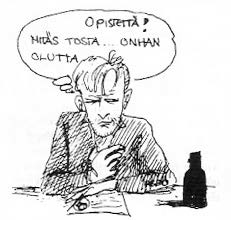
\includegraphics{onhanolutta.png}
\end{table}
\newpage
\section{Uutta tutkintosanastoa vanhoille} {\small \itshape ``Näin selität vanhemmalle tieteenharjoittajalle, mistä tutkinnossasi on kyse''}\vspace{0.5cm}
\begin{table}[h!]
	\begin{tabularx}{\textwidth}{lX}
		Fuksilaite &= Linux- tai Windows-läppäri, jonka jokainen fuksi saa opintojensa alussa, ja jonka vastineeksi edellytetään tunnollista opiskelua\\[5pt]
		Jory &= johtoryhmä; jokaisen kandi- ja maisteriohjelman suunnittelussa on nykyään mukana kaksi opiskelijaa, ja heillä on henkilökohtaiset varajäsenet\\[5pt]
		Kosu &= koulutussuunnittelija; se opintotoimiston tyyppi\\[5pt]
		Maisterioptio &= Kandiohjelma voi lähtökohtaisesti valmistaa useampaan kuin yhteen maisteriohjelmaan. Kandiohjelmassa suoritetut opinnot vaikuttavat siihen, mitkä optio-ohjelmat tai niiden opintosuunnat ovat mahdollisia.\\[5pt]
		Osasto &= laitoksen nimitys nykyään, mutta sisältäen vain henkilökunnan\\[5pt]
		Tavoiteaika &= opetusministeriön mielestä ihmisten pitäisi valmistua
		kandidaateiksi kolmessa ja maistereiksi yhteensä viidessä vuodessa\\[5pt]
		Toisen tieteenalan opinnot &= sivuaine (15, 25, 35 op tai näiden moninkerta)\\[5pt]
		Työelämäopinnot &= tutkintovaatimuksiin tulee nykyään sisältyä työelämäjakso ja asiantuntijatehtäviin valmentavia osuuksia vähintään 10~op\\[5pt]
		SISu &= kehitys\-kelpoinen opintojen\-suunnittelu\-työkalu
\end{tabularx}
\end{table}
\twocolumn

\twocolumn[\section{Yliopiston kurssiarvostelu\dots} {\small \itshape ``Yliopistolla arvostellaan kurssit numeroilla, korkeimpana arvosanana 5.''}\vspace{0.5cm}]

\noindent+ 5 erinomaiset tiedot\\
+ 4 kiitettävät tiedot\\
+ 3 hyvät tiedot\\
+ 2 tyydyttävät tiedot\\
+ 1 välttävät tiedot\\
0 hylsyhköt tiedot\\
– 1 heikot tiedot\\
– 2 erittäin heikot tiedot\\
– 3 vakuuttavan heikot tiedot\\
– 4 ohkooset tiedot\\
– 5 sangen ohkooset tiedot\\
– 6 verrattoman ohkooset tiedot\\
– 7 vallan erinomaisen ohkooset tiedot\\
– 8 hymyilyttävät tiedot\\
– 9 naurettavat tiedot\\
–10 sangen naurettavat tiedot\\
–11 peräti röhönaurettavat tiedot\\
–12 tiedot eivät enää edes naurata\\
–13 itkettävät tiedot\\
–14 sangen itkettävät tiedot\\
–15 merkilliset tiedot\\
–16 hyvin merkilliset tiedot\\
–17 erittäin merkilliset tiedot\\
–18 erittäin vakuuttavan merkilliset tiedot\\
–19 kummalliset tiedot\\
–20 hyvin kummalliset tiedot\\
–21 erittäin kummalliset tiedot\\
–22 sangen eriskummalliset tiedot\\
–23 lievästi kyseenalaiset tiedot\\
–24 suhteellisen kyseenalaiset tiedot\\
–25 hyvin kyseenalaiset tiedot\\
–26 erittäin kyseenalaiset tiedot\\
–27 vastaajan älyn kyseenalaistavat tiedot\\
–28 arvostelijan älyn kyseenalaistavat
tiedot\\
–29 väärältä vaikuttavat tiedot\\
–30 vääristyneet tiedot\\
–31 väärät tiedot\\
–32 sangen väärät tiedot\\
–33 harhaoppisilta vaikuttavat tiedot\\
–34 harhaoppiset tiedot\\
–35 hyvin harhaoppiset tiedot\\
–36 erittäin harhaoppiset tiedot\\
–37 vain vähän tietoa\\
–38 vain aavistuksen verran tietoa\\
–39 tuskin mitään tietoa\\
–40 ei tietoa

\twocolumn[\section{Opiskelutekniikkaa}]
FM:n tutkintoa varten vaaditaan vähintään
300~opinto\-pistettä. Niin kuin varmaan
tiedät, opinto\-pisteitä saat käymällä kursseja,
tenttimällä ja tekemällä harjoituksia.
Voit suhtautua opiskeluusi periaatteessa
kahdella tavalla: ajattelet 300~op:n kakkua
ja alat vähitellen suorittaa siitä pois palasia
tai alat oppia parhaasi mukaan tietoa,
ymmärrystä ja kykyä käyttää tietojasi. Jos
valitset pois\-suorittamisen, huomaat pian
pyrkiväsi yli siitä, mistä aita on matalin:
mahdollisimman paljon opinto\-pisteitä
mahdollisimman vähällä vaivalla.

Ehkä huomaat myös työskentelysi keskittyvän
tentteihin ja kun tentti menee pieleen, olet
aivan maassa: et saanutkaan opintopisteitäsi.
Kannattaisi ehkä kokeilla toista vaihtoehtoa.
Yritä ajatella opiskeluasi pitkänä
prosessina, joka jatkuu koko elämäsi ajan
tavalla tai toisella. Silloin sinun ei tarvitse
hermoilla jokaisen tentin takia. Kun vain
opiskelet ja opit asioita, ehdit kyllä tenttiä
kaiken tarpeellisen.
\subsection*{Palkitse itsesi}
Älä mieti enää, onko sinulla lahjoja
yliopisto-opiskeluun. Olet päässyt yliopistoon
ja nyt sinun on vain pelattava niillä
korteilla, joita kädessä sattuu olemaan.
On turha pelätä,
että joutuisit lopettamaan
opiskelun siksi, että et jossakin vaiheessa
enää ymmärrä mitään. Jos vain opiskelet
tunnollisesti
alusta alkaen, saat hyvän
pohjan ja pärjäät myöhemminkin. Ei kuitenkaan
pidä säikähtää, jos ei ihan kaikkea
ymmärrä. Vaikeimmat asiat tulevat sisäistettyä
paljon
myöhemmin kuin ne ensimmäistä
kertaa
esiintyvät.

Yliopistossa ei kukaan vaadi sinua opiskelemaan,
joten vastuu edistymisestäsi on
yksin sinun. Saattaa olla hyödyllistä tehdä
joitakin suunnitelmia. Opiskeluusi tulee
puhtia, jos sinulla on selviä tavoitteita joihin
pyrit. Helposti hahmottuvia tavoitteita
ovat tentit, lyhemmän tähtäimen tavoitteita
on myös hyvä olla.

Älä yritä liikaa, ja kun olet päässyt tavoitteeseesi,
palkitse itseäsi. Palkinto voi
olla jätskiannos, kuuma kylpy tai koira,
uudet kengät tai mitä tahansa. Kunnon
saavutuksen
jälkeen voi pitää rauhassa vapaatakin
ja nukkua kunnolla.

\subsection*{Tee lukukausista erilaisia}
Jos et pidä yksitoikkoisesta puurtamisesta,
koeta suunnitella lukukausista erilaisia.
Lue joskus enemmän muita tieteenaloja,
keskity harjoitustöihin tai lue itseksesi
loppukokeeseen. Muista, että opinto-oppaan
aikataulut ovat vain viitteellisiä, yksi
mahdollisuus monista.

Olet jo ehkä kuullut jonkun sanovan,
ettei luennoilla kannata käydä. Usein niin
onkin, mutta tässä niin kuin muissakin kysymyksissä
sinun täytyy tehdä tuskallinen
päätös itse: käydäkö vai ei? Luennoitsijan
opetuskyvyt, saatavissa oleva materiaali
yms.\,vaikuttavat valintaasi, samoin kuin
se, opitko paremmin kuuntelemalla vai lukemalla.
Luennoilla nukahteluun on muuten
hyvä lääke: muistiinpanojen tekeminen.
Jos kurssilla on luentomoniste tai
kirja, kirjoita avainsanoja ja luennon runkoa
marginaaleihin. Jos taas monistetta ei ole ja muistiinpanoja on joka tapauksessa
tehtävä,
älä kopioi suoraan luennoitsijan
kalvoja.
Mieti, mistä puhutaan ja yritä
kommentoida
hämäriä ranskalaisia viivoja.
Sen lisäksi, että pysyt hereillä, saatat
oppiakin jotain. Muista, että kysyminen on
sallittua -- jopa suotavaa. Jos luennoitsija
sekoaa konsepteissaan, se on hänen murheensa,
ei sinun.

Laskuharjoituksissa on hyvä käydä,
vaikkei luennoilla kävisikään, niissä nimittäin
todella oppii. Laskarit on vaikea paikka
monelle, koska niissä ``joutuu'' silloin
tällöin esittämään omia ratkaisujaan. Yritä
suhtautua alusta alkaen laskaritilaisuuksiin
rauhallisesti. Jos ilmoittaudut heti alussa
vapaaehtoiseksi tekemään tehtäviä, pelkosi
poistuu nopeasti ja voit keskittyä oppimiseen.

\subsection*{Valitse mieleisesi aikataulu}
Lukujärjestystä suunnitellessa on otettava
huomioon, että suuri osa opiskelusta on
omaa työtä: lukemista ja harjoitusten tekoa.
Kaikille matemaattisille aineille on tyypillistä,
että tuhansien sivujen kahlaamisen
sijasta
joutuu miettimään muutamaa riviä ja
soveltamaan niitä tehtäviin. Vaikka opetus
ei ehkä tällä hetkellä innosta luovuuteen
niin paljon kuin voisi, aineidemme opiskelu
pakottaa kyllä käyttämään päätä. Loogisuus
on valttia ja se lisääntyy ihmeesti
opiskelun myötä.

Tärkeää on löytää oikea asenne, joka ei
pidä mitään ongelmia ylitse\-pääsemättöminä.
Yritä oppia tuntemaan itsesi: älä
laiskottele,
mutta kun olet todella henkisesti
tai fyysisesti väsynyt, lepää tai tee jotain
muuta.
Toisen työ on toisen lepo. Anna itsellesi
aikaa opiskeluun. Kun opiskelet, älä
ajattele,
mitä kaikkea muuta sinun pitäisi
tehdä. Tekemättömät työt rasittavat aina
eniten. Yritä keskittää arkiset talousaskareet
ja kaupoissa juoksemiset. Kaupungissa
liikkumiseen tuhlaantuu yllättävän paljon
aikaa ja voimia. Monet opiskelijat noudattavat
virastoaikaa ja pitävät illat ja viikonloput
vapaata; toiset taas arvostavat sitä,
että voivat liikkua kaupungilla keskipäivällä
ja tehdä töitä milloin haluavat. Valitse
mieleisesi vaihtoehto. Tarkka aikataulu
auttanee, kun motivaatio ei ole parhaimmillaan.
Varmaa on joka tapauksessa, ettei
aamusta iltaan kannata tehdä töitä. Sitä ei
kestä erkinkään aivot.

Muista, että alussa on pakko oppia tylsiä
perusasioita, mutta mitä pitemmälle pääset,
sitä mielenkiintoisemmalta alasi alkaa
tuntua. Motivaatiota lisää vaihtoehtoinen
opiskelu: lue lehtiä ja kirjoja ja keskustele
asioista. Erityisen hyödyllistä on kuunnella
vanhempia opiskelijoita ja kysellä heiltä
kaikenlaista.

\subsection*{Toimi, älä nyhjää!}
Tässä oli joitakin hyviä neuvoja, joita
voit miettiä ja kokeilla. Huomaa kuitenkin,
että elämä on opiskeluakin tärkeämpää! Jos
sinun on tänä vuonna löydettävä itsesi tai
Suuri Rakkautesi tai tehtävä vallankumous,
tee se. Muuten voit katua myöhemmin.
Monet ovat rauhallisemman nuoruuden
elettyään ``syntyneet'' vasta ensimmäisen
tai toisen opiskeluvuoden aikana. Älä kuitenkaan
tule syyttämään ratkaisuistasi tätä
opasta.

\vspace{0.5cm}
\noindent\textsc{Helena Ahonen}

\twocolumn[\section{Mikä sinusta tulee isona?}]
Vaikka opinnot ovatkin vasta alkaneet,
on silti hyvä suunnitella myös opintojen
jälkeistä elämää. Yliopistosta ei valmistu
vain yhteen tiettyyn tehtävään, vaan mahdollisten
työpaikkojen kirjo on laaja myös
yksittäisten oppiaineiden sisällä. Omaa
uravisiota kannattaa lähteä toteuttamaan
jo opintojen alkuvaiheessa, sillä mitä aiemmin
sen aloitat, sitä varmemmin sen tavoitat.
Jos oma visiosi on utuinen tai keinot
sen toteuttamiseen ovat hukassa, niin anna
Urapalveluiden auttaa. Helsingin yliopiston urapalvelut tarjoaa opiskelijoille paitsi luentoja
ja oppaita, myös henkilökohtaista
ura- ja
työnhakuohjausta. Voit myös antaa CV:si
ammattilaisten luettavaksi ennen kuin liität
sen osaksi työhakemustasi.

\subsection*{Luennot}
Urapalvelut pitää lukukausien
aikaan useita luentoja urasuunnittelusta
ja työnhausta sekä työnhakuasiakirjojen
tekemisestä. Lisätietoa Urapalvelujen toiminnasta löytyy Guidesta
\url{https://guide.student.helsinki.fi/fi/tyo-ja-ura}.

\subsection*{Oppaat}
Rekry julkaisee oppaita työnhausta ja
harjoittelusta. Oppaat löytyvät paitsi Flammasta
(Hakemisto ja palvelut $\rightarrow$ Opiskelijalle
$\rightarrow$ Työelämään), niin myös painettuna Rekryn asiakaspalvelusta.

Helsingin yliopiston urapalvelut neuvovat sivulla \url{https://guide.student.helsinki.fi/fi/artikkeli/tyonhaku}, miten löydetään omat vahvuudet, kuinka tehdään tavallinen tai video-CV ja miten valmistautua haastatteluun. Myös ammattiliitto Tekniikan akateemiset tekevät vuosittain hyvän matemaattisluonnontieteellisille aloille suunnatun työnhakuoppaan, jonka löytyy osoitteesta: \url{http://teekkarintyokirja.tek.fi/}

\subsection*{CV-palaute}
Kun olet hakemassa työ- tai harjoittelupaikkaa,
sinua pyydetään lähettämään
työhakemus ja CV. Näiden asiakirjojen
perusteella työ- tai harjoittelupaikan antaja
karsii suurimman osan hakijoista. Eikö siis
kannattaisi pitää huolta näiden asiakirjojen
tasosta? Ennen kuin lähetät työhakemuksesi
ja ansioluettelosi työnantajalle, kannattaa
lähettää ne Rekryn ammattilaisten luettavaksi
ja kommentoitavaksi osoitteeseen
\url{careerguidance@helsinki.fi}. Haastattelukutsun
saaminen on tällä tavalla paljon todennäköisempää.

\subsection*{Henkilökohtainen neuvonta}
Urapalveluiden asiakaspalvelusta voit hakea
nopeat neuvot mieltäsi askarruttaviin
työelämäkysymyksiin.
Sieltä saat myös ohjausta
oikeille tiedonlähteille työnhakuun,
harjoitteluun, sijoittumiseen ja syventävien opintojen tutkielman (gradun)
toimeksiantoihin
liittyvissä asioissa. Kun
tarvitset hieman luentoja yksilöllisempää ohjausta, kannattaa varata aika yliopiston uraohjaajalle.

\subsection*{RekryNet ja opiskelijakirje}
Aiempi RekryForum on korvautunut
keväästä 2015 alkaen RekryNetillä, johon
nykyisin julkaistaan kaikki yliopiston opiskelijoille
ja vastavalmistuneille tarkoitetut
työ- ja harjoittelupaikat sekä pro gradu
-paikkoja. RekryNetin löytää kätevästi
osoitteesta \url{www.helsinki.fi/rekrynet}.
Urapalveluiden nettisivuilta löytyy
myös suora linkki Urapalveluiden opiskelijakirjeen
tilaamiseen.

\onecolumn
\subsection*{Yhteystiedot}
\begin{flushleft}Urapalvelut: \url{www.helsinki.fi/urapalvelut/}\\
Käyntiosoite: Fabianinkatu 33 (yliopiston päärakennus, 1. kerros) 00100 Helsinki\\
Postiosoite: PL3, 00014 Helsingin yliopisto\\
Puhelin: (02) 941 22125\\
Sähköposti: \url{careerguidance@helsinki.fi}
\end{flushleft}
\begin{figure}[!b]
	\centering
	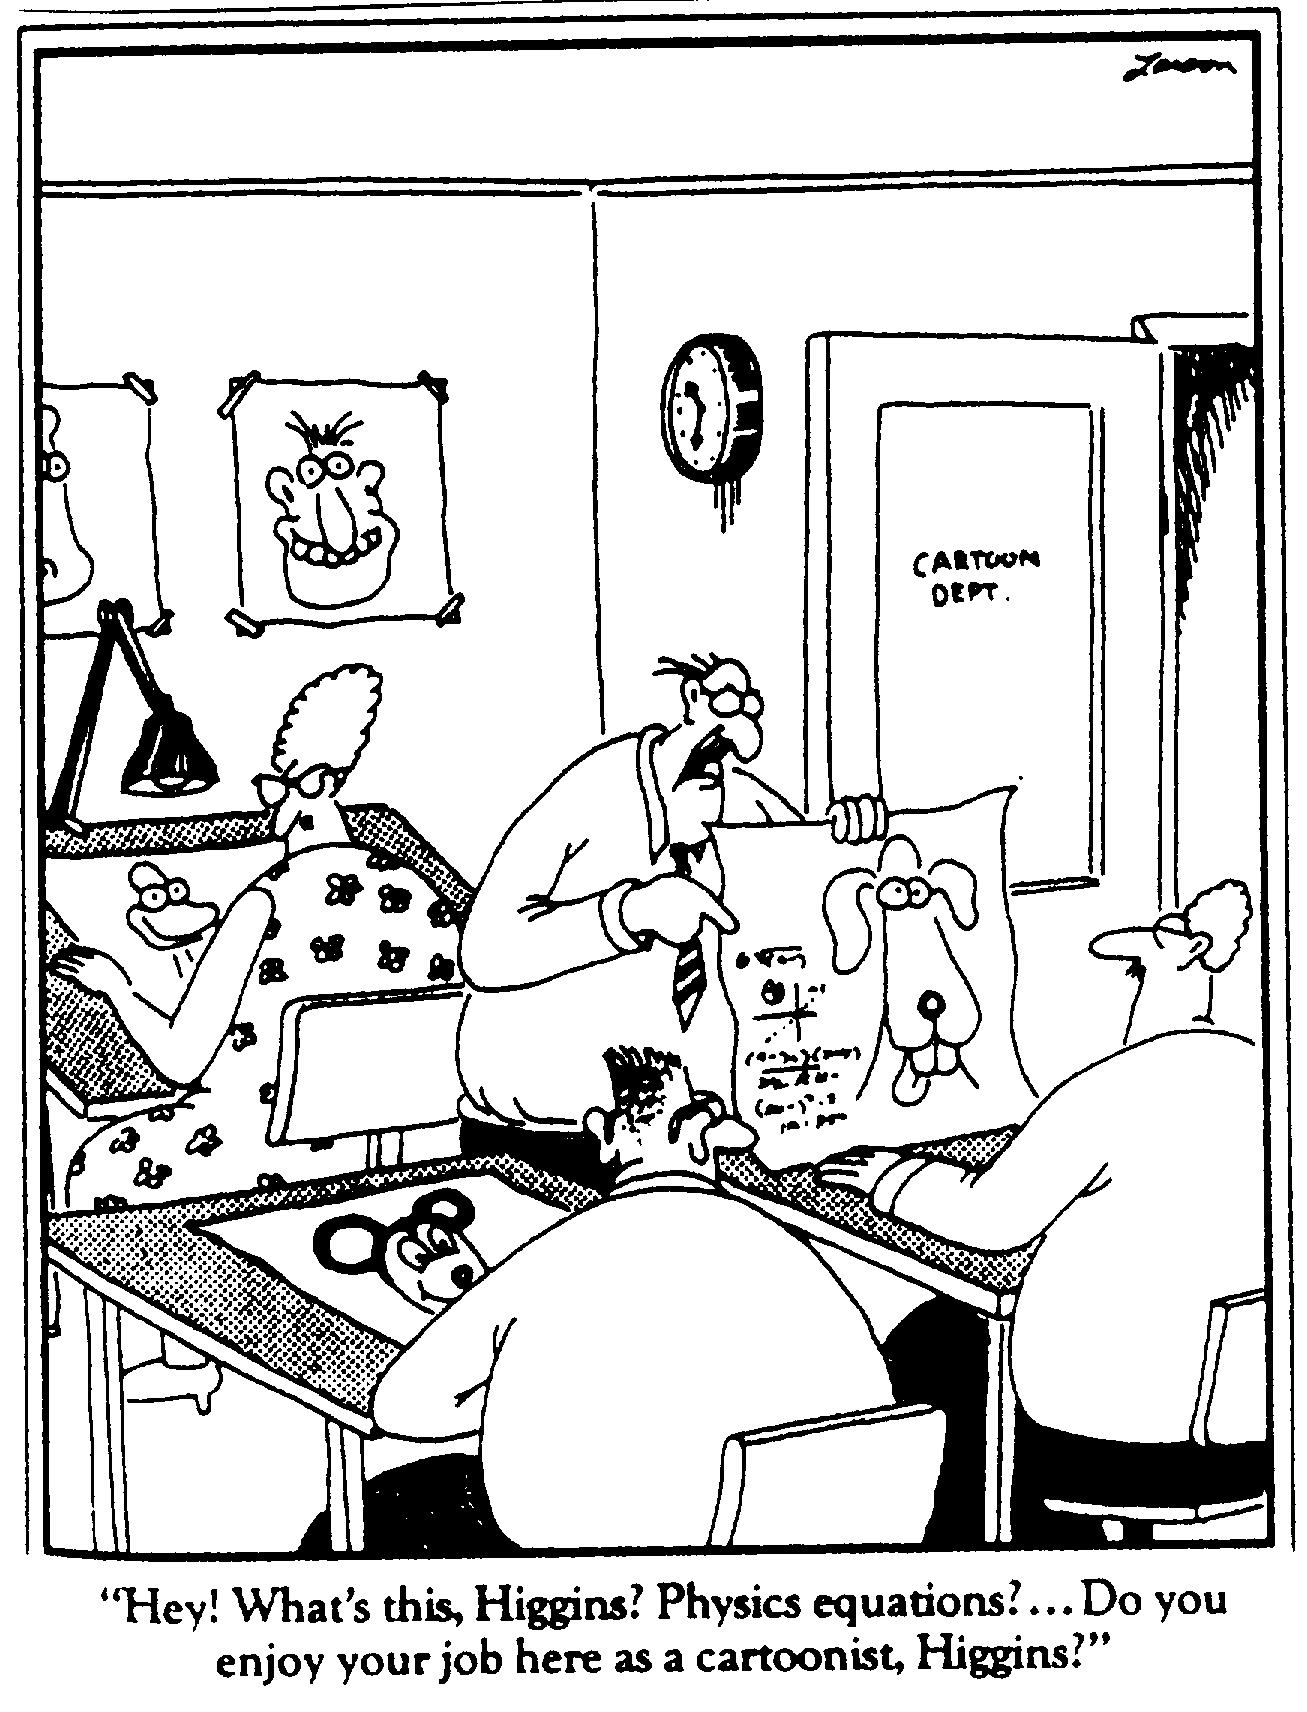
\includegraphics[width=0.8\textwidth]{higgins.png}
\end{figure}
\section{Tiedekunnan rakenne}
Tiedekunnan rakenne 1.1.2018 alkaen on esitetty oheisessa kuvassa. Tähdellä on merkitty ne toimielimet, joissa opiskelijoilla on edustus.

\vspace{0.5cm}
\begin{center}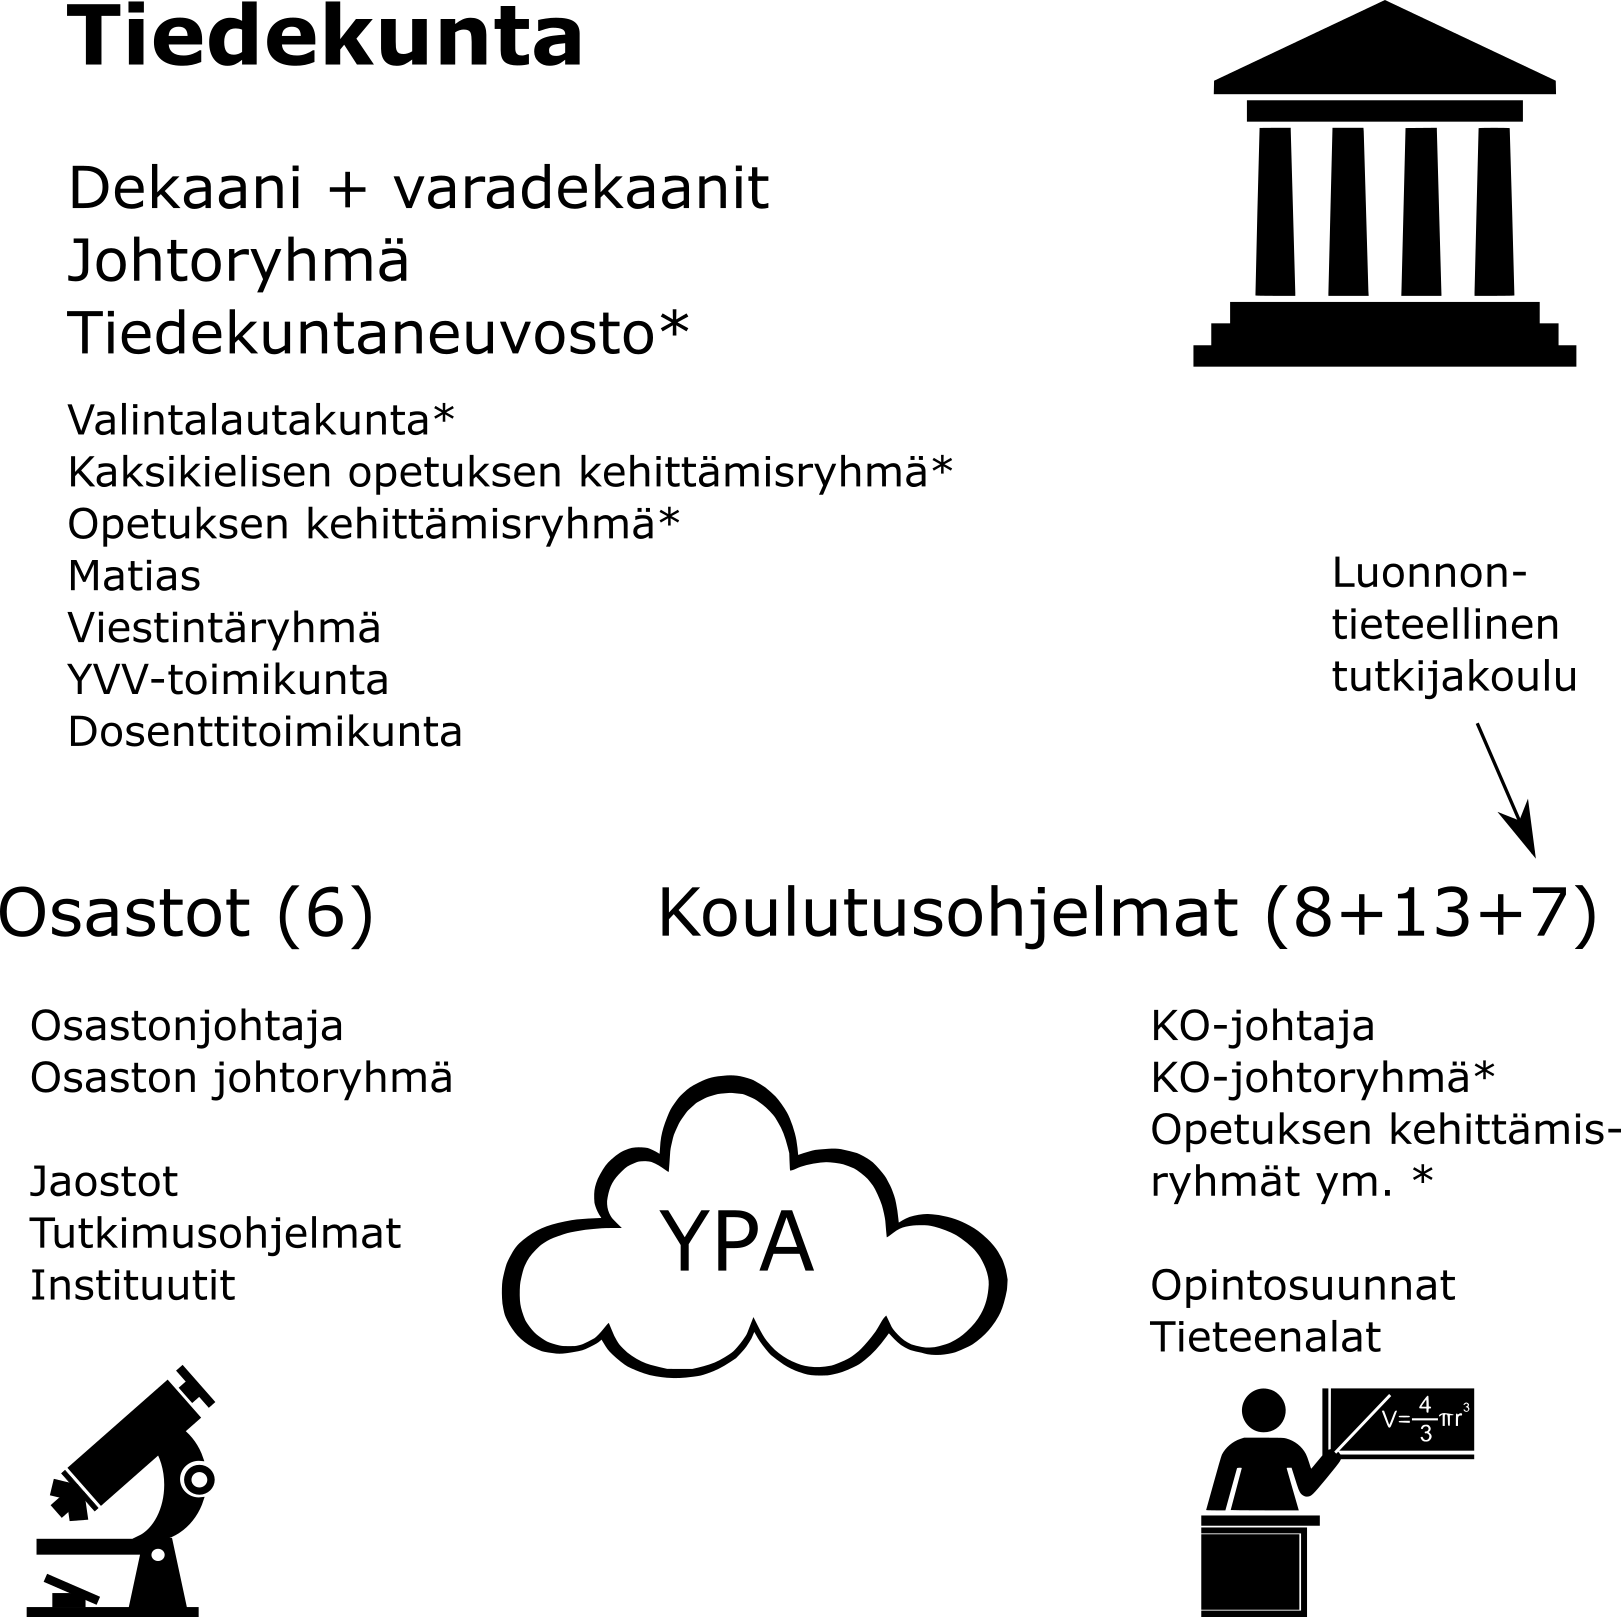
\includegraphics[width=0.75\textwidth]{uusitiedekunta.png}\end{center}

Matemaattis-luonnontieteellisessä tiedekunnassa toimivat seuraavat osastot (engl.\,\textit{department}). Osastot tulevat sinulle tutuiksi viimeistään siinä vaiheessa, kun alat tähyillä yliopiston työpaikka\-ilmoituksia.
\begin{itemize}
	\item Fysiikan osasto
	\item Geotieteiden ja maantieteen osasto (sis.\,Seismologian instituutti)
	\item Ilmakehätieteiden keskus INAR
	\item Kemian osasto (sis.\,Kemiallisen aseen kieltosopimuksen valvontainstituutti VERIFIN)
	\item Matematiikan ja tilastotieteen osasto
	\item Tietojenkäsittelytieteen osasto (sis.\,Tietotekniikan tutkimuslaitos HIIT)
\end{itemize}
 
\twocolumn
\subsection*{Yleistä koulutusohjelmista}
Kumpulassa opinnoissasi on runsaasti valinnanvaraa, sillä suurimmalle osalle kursseista voi osallistua vapaasti. Monista tieteenaloista on koottu myös valmiita 15, 25 tai 35~op opintokokonaisuuksia (ns.\,sivutieteenalat), joita saa liittää tutkintoonsa vapaasti -- toki opetussuunnitelman ja pysyväismääräysten asettamissa rajoissa.

Valinnaiset opinnot ja opintokokonaisuudet löytyvät kootusti Opiskelijan ohjeista: \url{https://guide.student.helsinki.fi/fi/valinnaiset-opinnot}

Kumpulassa voit valita opintosi seuraavista
kandiohjelmista:
\begin{itemize}
	\item Fysikaaliset tieteet
	\item Geotieteet
	\item Kemia
	\item Maantiede
	\item Matemaattiset tieteet
	\item Matematiikan, fysiikan ja kemian opettaja
	\item Science
	\item Tietojenkäsittelytiede
\end{itemize}

Myös seuraavien maisteriohjelmien kursseista voi löytyä sopivaa tarjontaa. Mikäli joku väittää sinulle, että maisterikursseille ei saa mennä ennen kuin kandidaatintutkinto on suoritettu, on hän väärässä. Tällaista linjausta oltiin puuhaamassa keväällä~2017 ns.\,Bologna-prosessin jälkimainingeissa, mutta opiskelijoiden vastustuksesta sitä ei lopulta kirjattu tutkintoja koskeviin pysyväismääräyksiin. Sen sijaan maisteriohjelmat voivat halutessaan kiintiöidä kurssipaikkoja omille opiskelijoilleen tai rajata osan kursseista vapaan osallistumisen ulkopuolelle (esim.\,kenttäkurssit ja pienryhmäopetuksen). Ylimääräisten opetuspaikkojen järjestäminen on monesti resurssikysymys, johon maisteriohjelmilla ei yksinkertaisesti ole varaa, ja tätä kannattaa kunnioittaa.

\begin{itemize}
	\item Alkeishiukkasfysiikka ja astrofysikaaliset tieteet
	\item Datatiede
	\item Elämäntieteiden informatiikka
	\item Geologia ja geofysiikka
	\item Ilmakehätieteet
	\item Kaupunkitutkimus ja -suunnittelu
	\item Kemia ja molekyylitieteet
	\item Maantiede
	\item Matematiikan, fysiikan ja kemian opettaja
	\item Matematiikka ja tilastotiede
	\item Materiaalitutkimus
	\item Teoreettiset ja laskennalliset menetelmät
	\item Tietojenkäsittelytiede
\end{itemize}

Lisää kursseja voit löytää Joustavan opinto-oikeuden kautta (JOO-opinnot), Helsinki Summer Schoolista tai Avoimen yliopiston piiristä.

Opiskeluita koskevat yleiset määräykset sekä opiskelijan oikeusturva linjataan yliopiston Tutkinto- ja oikeusturvajohtosäännössä (15~sivua) sekä Helsingin yliopiston tutkintoja ja opintoja koskevissa linjauksissa (16~sivua). Näistä asiakirjoista juontaa juurensa mm.\,sääntö, että laboratorio- ja ohuthie\-kurssit tulee saada päätökseen viimeistään vuoden kuluessa niiden aloituksesta, ja että tutkintotodistukseen merkitään enintään 10~\% tutkinnon laajuuden ylittäviä opintoja.

Ota siis linkit talteen!

\url{https://guide.student.helsinki.fi/sites/default/files/2017-07/Tutkinto_oikeusturvajohtosaanto_6_2017_su.pdf}

\url{https://guide.student.helsinki.fi/sites/default/files/2017-07/Liite%2C%20Helsingin%20yliopiston%20tutkintoja%20ja%20opintoja%20koskevat%20linjaukset.pdf}

\subsection*{Opetuksen kieli}
Yliopistolain \S~11 mukaisesti Helsingin yliopiston opetus- ja tutkintokielet ovat suomi ja ruotsi. Toisaalta yliopistolla on useita kansainvälisiä opiskelijoita, jotka opiskelevat englanniksi ja maksavat lukuvuosimaksua. On siis syytä täsmentää, mitä tarkoittaa ``opetuksen kieli'', ja millä perusteella se määräytyy.

Kumpulan kandiohjelmat ovat yksikielisiä ja maisteriohjelmat monikielisiä. Poikkeuksia on vain yksi -- Matematiikan, fysiikan ja kemian opettajan maisteriohjelma --, sillä aineenopettajan pätevyys edellyttää kotimaisen kielen erinomaista hallintaa.

Yksikielisissä kandiohjelmissa luento-opetus annetaan ohjelman kielellä (kotimaiset kielet tai englanti). Kotimaiskieliseen koulutusohjelmaan voi sisältyä englanninkielisiä osioita, joissa opetus on englanniksi. Silti opiskelijalla pitäisi olla aina mahdollisuus palauttaa laskarit ja tenttiä tentit kotimaisella kielellä.

Monikielisissä maisteriohjelmissa luento-opetus annetaan englanniksi, mutta näissäkin opiskelijoille tulisi tarjota mahdollisuus palauttaa laskuharjoitukset ja tenttiä tentit kotimaisella kielellä -- ainakin pakollisilla kursseilla. Jos kurssilla ei ole yhtään englanninkielistä opiskelijaa, vedetään opetus yleensä kotimaisella kielellä.

Jotta asia ei olisi liian yksinkertainen, voivat fysiikan ja kemian kandiopiskelijat toisen opiskeluvuoden syyslukukauden loppuun mennessä ilmoittautua suorittamaan kaksikielistä tutkintoa (ns.\,KaTu-opinnot), jolloin opinnoista vähintään 1/3 on suoritettava suomeksi ja ruotsiksi. KaTu-opinnot antavat pätevyyden toimia kahdella kielellä, ja niiden aikana suoritetaan myös CEFR:n C1-tason kielitesti.

Seuraavassa osiossa esitellään kandiohjelmia ja niiden kursseja tarkemmin. Löydä itsellesi oma suosikkisi!

\chapter{Matemaattiset tieteet}
\subfile{sections/matemaattiset_tieteet}

\chapter{Tietojenkäsittelytiede}
\subfile{sections/kapistely}

\chapter{Kemia}
\subfile{sections/kemia}

\chapter{Fysikaaliset tieteet}
\subfile{sections/fysikaaliset_tieteet}

\chapter{Geotieteet}
\subfile{sections/geotieteet}

\chapter{Maantiede}
\subfile{sections/maantiede}

\chapter{Opettajankoulutus}
\subfile{sections/opettajankoulutus}

\chapter{Kaikkea muuta}
\twocolumn[\section{Kieliopinnot}]
Kaikkien matemaattis-luonnon\-tieteellisessä
opiskelevien täytyy suorittaa tietty
määrä kieliopintoja. Ei, kielistä et pääse
eroon lukion käytyäsi -- tämä on joillekin
tuskallinen, toisille iloinen uutinen. Pakollisia
opintoja ovat toisen kotimaisen kielen,
vieraan kielen ja äidinkielen opinnot.
\begin{figure}[!b]
	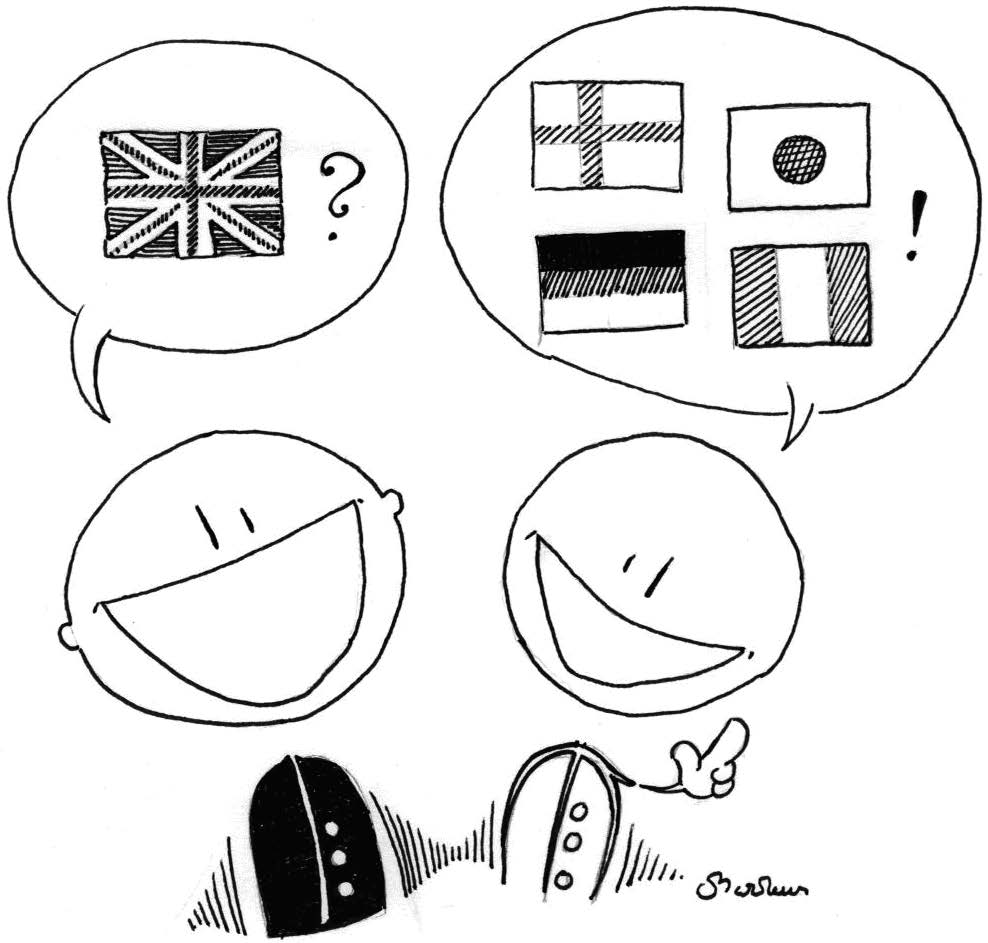
\includegraphics[width=\columnwidth]{kielijuttu.png}
\end{figure}

Äidinkieltä lukuun ottamatta kielten
opettamisesta huolehtii yliopistolla Kielikeskus. Kielikeskuksen
kurssitarjonta on varsin laaja. Voit aloittaa
ilman mitään esitietoja tai jatkaa siitä, mistä
lukiossa jäi kesken. Huomaa, että aivan
ummikoille tarkoitetut kurssit aloittavat
``Terve, mitä sinulle kuuluu?'' -tasolta. Jos
olet jo suorittanut parikin kurssia lukiossa,
niin kannattaa mennä vähän haasteellisemmalle
kurssille. Jos on epäselvyyttä, mille
tasolle mennä, voit mennä keskustelemaan
kielen opettajatuutorin kanssa. Kielikeskus
sijaitsee Fabianinkatu~26:ssa (F26) oppimiskeskus Aleksandrian ja opiskelijakirjaston
vieressä. Suurinta osaa kursseista
ei kuitenkaan pidetä tässä rakennuksessa,
vaan pitopaikat on hajautettu pitkin kaupunkia
yliopiston eri rakennuksiin. F26:ssa
sijaitsevat opetustilojen lisäksi Kielikeskuksen
opintotoimisto (sisääntuloaula, 1.\,krs) sekä hallinto. Kielikeskuksen opettajien
työtilat ovat puolestaan Vuorikatu~5:ssä.
Oppimiskeskus Aleksandriassa (F28) sijaitsevat
Kielikeskuksen itseopiskelutilat,
joissa voi opiskella itsenäisesti 50~kieltä ja
saada itseopiskeluohjausta.
\subsection*{Pakolliset kieliopinnot}
\subsubsection*{Vieraan kielen opinnot (4~op)}
Vieraan kielen tutkintovaatimusten mukaiset
taidot voi osoittaa joko osallistumalla
kurssille tai suorittamalla kurssin korvaavan
kokeen. Vaihtoehtoisia kieliä ovat
ainakin englanti, arabia, italia, japani, kiina, portugali, ranska, saksa, tanska, venäjä ja viro. Jos uskoo taitoihinsa, kannattaa
toki kokeilla kurssia korvaavaa koetta
-- osa opiskelijoista sen läpäiseekin.
Jatkoteksti koskee englannin opintoja,
joilla varmaan useimmat kuittaavat
pakollisten kieliopintojen osuuden.
Muiden kielten käytännöt saattavat
kurssin korvaavan kokeen tai kurssien
osalta olla hieman erilaiset.
\begin{figure*}[!b]
\centering
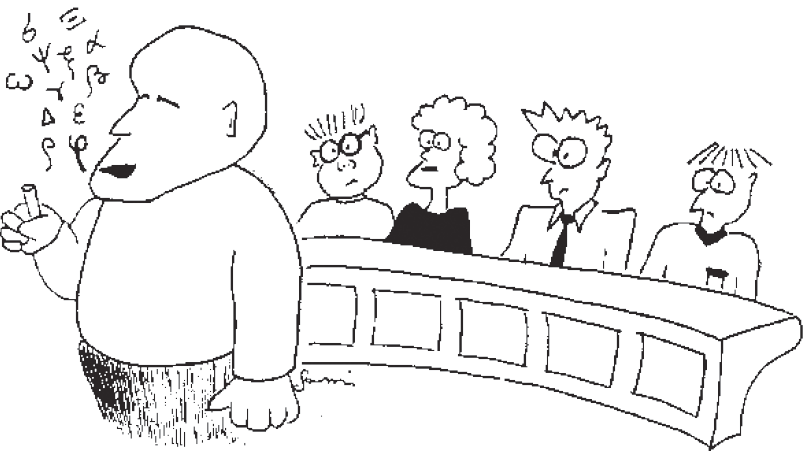
\includegraphics[width=\textwidth]{kieliluento.png}
\end{figure*}
Kurssin korvaava koe koostuu kolmesta
osasta: ykkösosassa testataan lukemisen
ja kirjoittamisen hallintaa, kakkososassa
kuullunymmärtämistä ja viimeinen osio
on kymmenminuuttinen haastattelu, jonne
pääsee vain, jos kaksi ensimmäistä osaa
sujuivat hyvin. Jos kaikki osiot menivät hyvin, kuittautuvat pakolliset kieliopinnot
tällä, muuten joutuu käymään koetuloksista
riippuen yhden tai kaksi kurssia.

Jos kurssin korvaava koe meni huonosti
tai ei muuten vaan innosta, voi kieliopintojen
neljä opintopistettä suorittaa myös
osallistumalla kursseille. Kurssit saa valita
melko vapaasti myös edistyneemmistä
kursseista, mutta yleensä ensimmäisenä
suoritetaan perustason kurssi (2~op), jolla
harjoitellaan kirjoittamista, tekstien lukemista
ja jutellaan. Tämän jälkeen valitaan
kurssitarjonnasta yksi kahden opintopisteen vähän
edistyneempi kurssi, joita löytyy eri
painotuksilla. Kursseista pääsee kyllä läpi,
vaikka joku osio ei aluksi oikein sujuisikaan
-- opettajien kanssa voi jutella mahdollisista
lisätöistä. Vieraan kielen opinnot
kannattaa suorittaa heti opiskelun alussa,
sillä kielitaitoa tarvitaan varsinkin luettaessa
vieraskielisiä kurssikirjoja. Muutenkin
vähintään kelvolliset englannin kielen
taidot ovat ML-aineiden aloilla käytännön
välttämättömyys.

\subsubsection*{Toisen kotimaisen kielen opinnot (3~op)}
Vieraan kielen tavoin voi tämänkin opintojakson
suorittaa kahdella tavalla: osallistumalla
kurssille tai suorittamalla kolmiosaisen
kielikokeen. Koe on vaikeampi
kuin vieraassa kielessä. Koetta suositellaan
niille, jotka ovat saaneet ylioppilaskokeessa
vähintään Magnan ja/tai harjoittaneet
kielitaitoaan esim.\,työelämässä. Kokeessa
edellytetään lukion oppimäärän lisäksi perehtymistä
opiskelualan sanastoon, termeihin,
suulliseen ilmaisuun sekä sujuvaan
kirjoittamiseen. Vaikka tämä kuulostaa
hankalalta, kannattaa aina yrittää.

Koe on kolmiosainen. Ensimmäisessä
osassa testataan oman alan keskeisen
terminologian ja peruskieliopin hallintaa.
Jos tästä pääsee läpi, saa osallistua kirjoitus-
ja suulliseen kokeeseen, jossa pitäisi
osata keskustella omaan alaan liittyvistä
kysymyksistä. Useimmat suorittanevat
opintojakson kolme opintopistettä kuitenkin
kurssilla, jonka päätteeksi on suullinen ja
kirjallinen koe. Täälläkin kannattaa kysellä
lisätöitä, jos koe ei ensimmäisellä kerralla
oikein sujunut -- opettajat ovat yleensä ihan
mukavia ja yhteistyöhaluisia, joten kurssin
saa kyllä aina jotenkin suoritettua! Toinen
kotimainen kannattaa suorittaa aika pikaisesti,
ainakin niin nopeasti, etteivät vanhat
opit ehdi unohtua. Suositeltava
paikka on toinen opiskeluvuosi tai jo ensimmäisen vuoden
kevät.
\subsubsection*{Äidinkielen opinnot (3~op)}
Nykyiseen tutkintoon kuuluu jonkin
verran äidinkielen opintoja, joiden järjestämisestä
vastaa tiedekunta. Käytännössä
tämä tarkoittaa, että äidinkielen opinnot
suoritetaan tiedekunnassamme esimerkiksi LuK "-tutkielman,
seminaariesitelmän tai jonkin pääaineen
kurssin yhteydessä niin, että äidinkielen kolmen
opintopisteen suullisen ja kirjallisen viestinnän
vaatimukset täyttyvät. Käytännöt
ovat vasta muotoutuneet, joten omia ideoita,
vaihtoehtoja ja palautetta kannattaa
esittää -- parhaimmillaan voi jopa päästä
vaikuttamaan oman kandiohjelman tuleviin käytäntöihin!
\subsection*{Kursseista}
Kielikeskuksen opinto-oppaassa on ilmoittautumisohjeiden
ja kurssitarjonnan lisäksi myös muuta käytännön
tietoa Kielikeskuksen opetuksesta,
itseopiskelusta ja kielten verkko-opiskelumateriaaleja.
Kursseille ja kokeisiin ilmoittaudutaan
pääsääntöisesti WebOodissa.

Ilmoittautuminen alkaa kahta viikkoa
ennen ja päättyy viikko ennen periodin
alkamista. (Koeilmoittautuminen päättyy
viikkoa ennen koetilaisuutta. Tarkista poikkeukset
WebOodista.) Tietokoneen ääressä
ei tarvitse olla heti kurssi-ilmoittautumisen
alkaessa; riittää, että ilmoittaudut ajoissa!

Älä kuitenkaan ilmoittaudu turhaan ja
muista peruuttaa ilmoittautumisesi, jos et
voikaan osallistua opetukseen. Liian moni
opiskelija jää turhaan ilman kurssipaikkaa vain siksi, että itsekkäät jurpot jättävät
peruuttamatta saadun paikkansa kurssilla,
vaikka eivät osallistu opetukseen.

Ensimmäiselle luennolle on syytä mennä
tai todennäköisesti menettää paikkansa
jollekin jonottajalle. Aikaisemmin kannustettiin
jonottajiakin menemään ensimmäiselle
kokoontumiskerralle, jos todella oli
innostusta päästä kurssille. Näin ei ole enää,
vaan nykyisin WebOodissa ilmoittautumista
painotetaan. Tästä huolimatta ensimmäiselle
kokoontumiskerralle menevä jonottaja
saattaa päästä kurssille, sillä kaikkihan
on mahdollista, jos oikein yrittää. Ensimmäisellä
luennolla selviävät myös kurssin
yleiset järjestelyt ja käytännöt. Kannattaa
huomata, että suhtautuminen poissaoloihin
saattaa olla ihan erilainen kuin omassa
tiedekunnassa! Yleinen käytäntö Kielikeskuksen
kursseilla on vähintään noin 80~\%:n
läsnäolovelvollisuus ja kurssiin kuuluvien
tehtävien suorittaminen.

Varsinainen kurssin sisältö riippuu paljon
kurssin vetäjästä. Joillain paahdetaan
kielioppia, toisilla vain keskustellaan ja
lueskellaan tekstejä. Tunteja on yleensä
muutama viikkoa kohden, ja vetäjät voivat
poiketa hyvinkin paljon pölyisistä yliopistoluennoitsijoista.
Kannattaa kysyä jo kurssin
käyneiltä opiskelijoilta, mitä opettajaa
he suosittelevat. Kurssien ja loppukokeiden
vaikeustaso ei ole mahdoton -- jos aiemmat
taidot ovat heikot, joutuu tekemään hiukan
töitäkin, mutta suurin osa opiskelijoista
pärjää vain pienellä kertauksella. Lisäksi
monissa kielissä järjestetään valmentavia
ja kertauskursseja, jos tiedot kaipaavat
päivittämistä ennen varsinaiselle kurssille
menoa.

\subsection*{Muuta kielellistä toimintaa}
Kurssien ja korvaavien kokeiden lisäksi
Kielikeskuksella järjestetään myös vapaaehtoista,
sosiaalista toimintaa. Mikäli
olet kiinnostunut kielitaidon harjoittelusta
muiden ihmisten kanssa, voivat viikoittaiset
Kieliklubit olla sinulle oikea paikka.
Ryhmässä on yleensä kyseistä kieltä äidinkielenään
puhuva henkilö joka osaa auttaa
kieleen liittyvissä kysymyksissä. Kieliklubeihin
osallistuminen kannattaa sillä voit
saada uusia ystäviä!

Kieliklubien lisäksi Kielikeskus ylläpitää
Kielikaveri-listaa jonne voi laittaa
ilmoituksen tai etsiä ilmoituksien joukosta
henkilöä joka haluaa harjoittaa kieltä kanssasi.

\twocolumn[\section{Yleistä höpötystä sivutieteenaloista}]
Toisten tieteenalojen lukeminen on yksi niitä
asioita, joissa sekakäyttö kannattaa. Eikö
olisikin kiva ajatus, että olisit yksilö? Valmistuttuasi
et tulisi olemaan osa täsmälleen
samanlaisia tutkintotodistuksia heiluttavien
kloonien armeijaa, mistä saattaa olla iloa
esimerkiksi työnhaussa. Jännillä sivutieteenaloilla
ilostutat elämääsi muutenkin, jouduthan
joka tapauksessa aika monta vuotta elämästäsi
yliopistolle uhraamaan.
\begin{figure*}[!b]
	\centering
	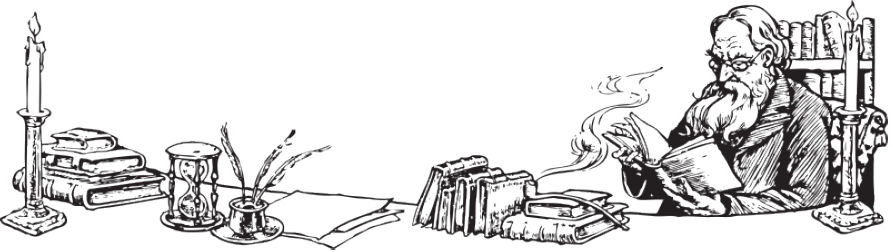
\includegraphics[width=\textwidth]{sivuaineproffa.png}
\end{figure*}

Nyt opiskelijana kannattaa hyödyntää
sekin etu, että pääset käsiksi moniin eri kursseihin.
Valmistuneena voi olla huomattavasti
hankalampi puljata itselleen oikeus
johonkin tiettyyn opintokokonaisuuteen.
Toteuta siis haaveesi jo nyt eikä vasta vapaavalintaisen
ikäkriisin koittaessa.
\subsection*{Mitä kaikkea voi lukea?}
Tässä oppaassa mainitaan monia vekkuleita
tieteenaloja, joita on mahdollista
suorittaa myös sivutieteenaloina.
WebOodi, tieteenalojen nettisivut tai ainejärjestöjen
sivut antavat vinkkejä sivutieteenalakokonaisuuksista
ja muista kyseiseen alaan
liittyvistä spesialiteeteista. Muista myös
muut tiedekunnat!

Valinnaiset opinnot ja opintokokonaisuudet löytyvät kootusti yliopiston sivuilta:

\noindent\url{https://guide.student.helsinki.fi/fi/valinnaiset-opinnot}

Tutkinnosta riippuu, kuinka paljon voit
tehdä toisia tieteenaloja ja millaisia suositellaan.
Tutkintorakenteesi voit kaivaa esille
SISusta, Wikistä tai vaikka tämän oppaan lehdiltä.
Joihinkin tieteen\-aloihin pitää hakea opinto-oikeutta. Osa on ns.\,vapaita tieteenaloja,
eli sen kun rupeat vääntämään opintokokonaisuutta,
kun siltä alkaa tuntua. Joitakin
tieteenaloja ei voi valita ollenkaan:
esimerkiksi lääkis ei halua antaa ymmärrettävistä
syistä sinulle valelääkäriyden vaatimia
taitoja.

Avoimen yliopiston kautta pääsee käsiksi
sellaisiin tieteenaloihin, joihin olisi
muuten hankalaa tai jopa mahdotonta saada
opinto-oikeutta. Lisäksi tutkinto-opiskelijan
on kesäisin ilmaista opiskella avoimessa,
jee!
\subsection*{Koskeeko tämä jo minua, täh?}
Tulevaisuuttaan kannattaa
alkaa miettiä, kunhan suunnilleen
on fuksivuodesta selvinnyt. (No pun intended.)
Vanhemmilla opiskelijoilla ja ainejärjestöjen
nettisivuilla saattaa olla kiinnostavia
vinkkejä, joten myös kannattaa alkaa
tutkia ympäristöään. Tämä hoituu esimerkiksi
saunailloissa höpisemällä.

\vspace{0.5cm}\noindent\textsc{Mari Teinilä}

\twocolumn[\section{Joopa JOO}]
Eikö matematiikka, taloustiede tai muut Helsingin
yliopiston tarjoamat kokonaisuudet nappaa? Niiden
sijaan voit käyttää hyväksesi JOO-opintoja, eli Joustavaa
Opinto-Oikeutta. JOOn avulla voit suorittaa opintoja
missä tahansa suomen korkeakoulussa. Kiinnostaisiko
vaikkapa Aallon konetekniikan kokonaisuudet? Tai miltä
tuntuisi Maanpuolustuskorkeakoulun opinnot?

Ensimmäisenä JOO-opinnot kannattaa
suunnitella huolella ja ajoissa -- hakuprosessissa
voi mennä jonkin verran aikaa!
Ensimmäisenä tarvitset puollon yliopiston
puolelta. Käytännössä JOO-opintojen pitää
siis sisältyä järkevästi tutkintoosi ja olla perusteltuja.
Tämä sen vuoksi, että tiedekunta
maksaa opintosi muissa korkeakouluissa,
eikä se ole aivan ilmaista! Haku tapahtuu
sähköisellä lomakkeella, joka löytyy osoitteesta
\url{https://haku.joopas.fi}. Tämän jälkeen asia
siirtyy koulutusohjelman yhteyshenkilölle -- hänen
tietonsa löytyvät Opiskelijan ohjeista
(toivottavasti!) -- ja paperit lähtevät rullaamaan.

No mitäs sitten voisi opiskella muualla?
Esimerkiksi fyysikoiden lienee melko
luonnollista saada oikeus opiskella
Aallon teknillisellä fysiikalla (kuitenkin vain sellaisia aloja,
joita yliopisto ei tarjoa), kun taasen
Maanpuolustuskorkeakoulu saattaa vaatia
jo enemmänkin perusteluja! MPKK:kin
tarjoaa mielenkiintoisia kokonaisuuksia,
kuten johtamiskoulutusta sekä strategiaa.
Rajoituksia on melko paljon, esimerkiksi
Taideteollisesta korkeakoulusta on melko
vaikeaa itkeä paikkaa muille kuin teoriaja
historiakursseille (lisäksi voidaan vaatia
työnäytekansiota) ja MPKK:n monet
kurssit ovat luonnollisesti varattuja vain upseeri\-opiskelijoille. Käytännössä yliopistot
luonnollisestikin tarjoavat paikkoja
ensisijaisesti omille opiskelijoilleen, joten
joillakin aloilla kurssit saattavat täyttyä
nopeasti! JOOssa ovat mukana kaikki suomen
yliopistot ja korkeakoulut, pois lukien
ammattikorkeakoulut -- valitse omasi!

\begin{figure}[!b]
	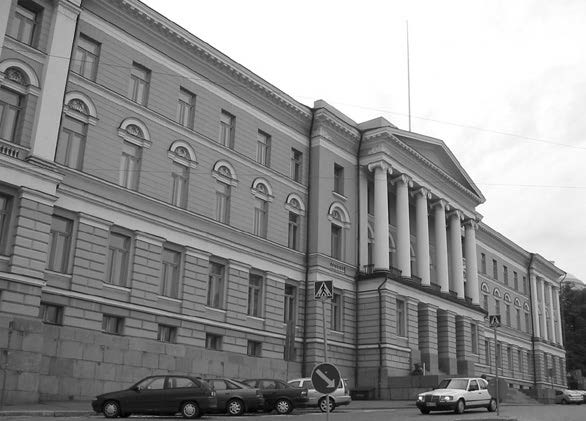
\includegraphics[width=\columnwidth]{paarakennus.png}
\end{figure}
Lisätietoja on saatavilla opintotoimistosta,
sekä (hyvin kattavasti ja helpommin!)
osoitteessa \url{http://www.joopas.fi}. Myös
tiedekunta tarjoaa neuvontaa lähettämällä
mailia \url{ml-neuvonta@helsinki.fi}.

\vspace{0.5cm}\noindent\textsc{Risto Karinkanta}

% kirjallisuutta poistettu 2018 painoksesta!
\chapter{Opiskelijaelämää}
\twocolumn[\section{Opiskelijajärjestöt}]
Järjestötoiminta Helsingin yliopiston ja sen
ylioppilaskunnan piirissä on erittäin monimuotoista ja
runsasta: voit liittyä kymmeniin erilaisiin järjestöihin
poliittisista ryhmittymistä harrastusjärjestöihin. Mikäli
vapaaehtoinen ja yleensä myös vapaamuotoinen
toiminta kiinnostaa, olet aina tervetullut mukaan!

\subsection*{Ylioppilaskunta}
on meitä kaikkia yhdistävä asia, siihenhän
kuuluvat automaattisesti kaikki perustutkinto-
opiskelijat. HYYn piirissä voi
harjoitella politikointia edustajistossa, kun
päätetään konkreettisistakin asioista. Toinen
vaikuttamismahdollisuus on osallistua
valiokuntien toimintaan. Niissä puidaan
asioita hieman pienemmällä mittakaavalla,
ja kenen tahansa on käytännössä mahdollisuus
osallistua niiden kokouksiin. Valiokunnat
eivät välttämättä ole niin pelottavan
virallisia kuin miltä nimi kuulostaa, toiminta
voi vaihdella tapahtumavaliokunnan varsin
rennosta menosta vähän virallisempiin kokouksiin
opintovaliokunnassa.
\subsection*{Osakunnat}
ovat ajalta ennen
HYYtä. Ne kokoavat -- ainakin periaatteessa
-- samalta alueelta Helsinkiin tulleet
opiskelijat yhteen. Käypä katsomassa, löydätkö
vanhoja tuttuja kotiseudultasi! Osakunnat
pitävät yllä akateemisia perinteitä:
pöytäjuhlia, wanhoja tansseja, laulua\dots
Suurin osa toiminnasta on kuitenkin epävirallista
ja rentoa. Saatat jopa tutustua muissa
tiedekunnissa ja tieteenahjoissa opiskeleviin
ihmisiin. Koosta ja varallisuudesta riippuen osakunnat tarjoavat myös asuntoja
ja stipendejä niitä kaipaaville.
\subsection*{Ainejärjestöt}
taasen muodostuvat saman aineen opiskelijoista.
Yhteishenkeä kohotetaan järjestämällä
bileitä, ekskursioita ynnä muita
tapahtumia. Näiden lisäksi ainejärjestöt
hoitavat tärkeää virallista tehtävää: ne ajavat
opiskelijoiden etua koulutusohjelmissa ja tiedekunnissa
sekä ovat mukana opiskeluolosuhteiden
kehittämisessä.

Näiden lisäksi löytyy siis myös leegio
harrastusjärjestöjä, poliittisia järjestöjä, uskonnollisia
järjestöjä, urheiluseuroja, kuoroja,
teattereita ja niin edelleen. Lisätietoa
näistä löydät Ylioppilaskalenteristasi sekä
yliopiston kotisivuilta, unohtamatta järjestöjen
omia tiedotusläystäkkeitä, lehtiä ja
kotisivuja.

\vspace{0.5cm}\noindent\textsc{Aku Valtakoski}
\twocolumn[\section{Ainejärjestöelämää}]
Aluksi menee kovasti aikaa tutustuessa
kanssaopiskelijoihin, niin fukseihin kuin
vähän pidempään opiskelleisiinkin. Käymällä
erilaisissa ainejärjestön tapahtumissa
tutustuu pikku hiljaa ydinporukkaan -- samoin
opiskelijahuoneet ovat
erinomaisia paikkoja kehittyä paikalliseksi
ihmistuntijaksi. Parhaiten ajan tasalla pysyt
kuitenkin käymällä hallituksen kokouksissa.
Älä huoli, ne eivät yleensä ole niin tylsiä
kuin miltä sana kuulostaa.

Kokouksissa päätetään likimain kaikesta
tulevasta aktiviteetista. Sen lisäksi näet
siellä, kuka on kukin ainejärjestössä. Saatat
päästä itsekin vaikuttamaan päätöksiin
eli siihen, mitä tapahtuu, missä ja milloin.
Intosi on tervetullutta: tilaa on aina sellaiselle,
joka on valmis pistämään tarmonsa
peliin yhteisen toiminnan järjestämiseksi.
Voin myös taata, että hauskaa on aina tarjolla,
myös ahertamisen ohessa!

Ja ainejärjestötoiminnasta on hyötyä.
Ihan oikeasti. Hauskanpidon ohella oppii
yhtä sun toista erilaisten tapahtumien ja
projektien organisoimisesta, virallisesta
kokouskäytännöstä ja vaikkapa organisaatioiden
raha-asioiden hoitamisesta. Tärkein
ainejärjestötoiminnan anti on kuitenkin sen
tuomat sosiaaliset taidot: opit toimimaan
erilaisten ihmisten kanssa yhteisten tavoitteiden
saavuttamiseksi sekä luot yhteyksiä,
verkostoidut. Kaikki taitoja, joita nykypäivän
työmaailmassa tarvitaan.
\begin{figure}[!b]
	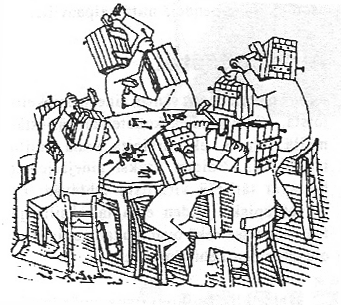
\includegraphics[width=\columnwidth]{lautapaa.png}
\end{figure}

Pieni varoituksen sana on kuitenkin paikallaan
ennen kuin ryntäät suin päin ainejärjestöjen
maailmaan: järjestötoiminta on
erittäin addiktiivista. Harvalle riittää vain
yksi järjestö, ja pian huomaat pääaineesi
olevan ``Limes'' ja kerääväsi tyhjiä pulloja
bileissä, joita et ole järjestämässä. Aseta
asiat siis tärkeysjärjestykseen -- ainejärjestössä
toimiminen vie aikaa, ja todennäköisesti
vaikuttaa opiskelutehokkuuteesi.
Myös järjestön toiminnan kannalta on tärkeää,
että aktiivit ovat riittävän omistautuneita
asialleen. Toiminnassa mukana olemisen
vaatima ajan uhraus ei kuitenkaan
ole liian suuri, ja on aina sen arvoinen.

Tiivistettynä: järjestötoiminta on hauskaa.
Älä siis fakkiudu vaan tule mukaan!

\vspace{0.5cm}\noindent\textsc{Reko Hynönen}

\twocolumn[\section{HYY}]
HYY, Matlu, Limes, aine\-järjestö\dots
Opintojesi alussa ihmettelet varmasti,
että mihin oikein tarvitaan noin montaa
hassun\-nimistä organisaatiota, jotka kehuvat
valvovansa etujasi. Onko niiden toiminta
jotenkin ristiriitaista? Onko opiskelijan
asema Suomessa, yliopistolla, tiedekunnassa
tai koulutusohjelmissa todella niin huono, että
tarvitaan noin monta toimijaa?
\begin{figure}[h]
	
\includegraphics[width=0.8\columnwidth]{hyylogo.png}
\end{figure}

Vastaus on kyllä ja ei. Opiskelijoiden
eduista yhteiskunnassa ei huolehdi päätoimisesti
kukaan muu kuin ylioppilaskunnat
ja ylioppilaskuntien liitto SYL, vaikka aina
eduskuntavaalien lähestyessä toisenlaista
viestiä kuuluisi useammaltakin taholta. Ja
koko yliopiston tasolla on paljon näkymättömissä
olevaa toimintaa, satamäärin suunnittelijoita
ja harmaata hallintokoneistoa,
jonka liikkeitä ylioppilaskunta ja hallinnon
opiskelijaedustajat vahtivat ja yrittävät ennakoida
ja vaikuttaa ajoissa. Vierivä lumipallo
on helppo pysäyttää kun se on pieni,
lumivyörylle ei kukaan voi enää mitään.

Tiedekuntatason asioista huolehtii tiedekuntajärjestö
Matlu ja koulutusohjelmatason
asioista ainejärjestö, loogista, eikö totta?
Näistä löydät lisää tietoa muualta tästä
oppaasta. Ja niistä ristiriidoista\dots eri edunvalvojatahot
eivät kiistele sielustasi tai
ruumiistasi, ajastasi ehkä. Organisaatiot ja
järjestöthän eivät sinällään tee mitään, vaan
ihmiset tekevät, toimivat, järjestävät, ottavat
selvää, suunnittelevat ja toteuttavat.
\subsection*{Palveluita jäsenille ja järjestöille}
Ylioppilaskunta tarjoaa jäsenilleen monenlaisia
palveluita, joista pääset osalliseksi
jäsenmaksun maksamalla:
\begin{itemize}
\item YTHS tarjoaa edullisia ja laadukkaita
terveydenhoitopalveluita.
\item Saat Ylioppilaskalenterin, joka on
samalla myös hyödyllinen opiskelijan
tietopaketti.
\item Saat alennusta opiskelijalounaasta ja kauko\-liikenne\-matkoista.
\item Saat kotiisi Ylioppilaslehden.
\end{itemize}
Vieläkin enemmän saat HYYn jäsenyydestä
irti, jos osallistut jonkin sen piirissä
olevan järjestön toimintaan. Yli 260~järjestön
joukosta löytyy jotain jokaiseen makuun:
on ainejärjestöjä, roolipeliseuroja, salamurhaajia, osakuntia, kuoroja ja paljon
muutakin. Ylioppilaskunta tukee näiden
toimintaa vuodessa yli miljoonalla eurolla.
Se tarjoaa niille mm.\,avustuksia, tiloja ja
koulutusta. Suurelta osin HYYn tuen ansiosta
voit esimerkiksi istua iltaa Klusterilla,
käydä eri järjestöjen saunailloissa -- tai
vaikka lukea tätä opasta.
\subsection*{Kaivopihan keisarikunta}
HYY on mitä todennäköisimmin maailman
rikkain ylioppilaskunta. Urbaanit
legendat kertovat kyllä jostain Latinalaisen
Amerikan ylioppilaskunnasta,
jonka omistamilta mailta olisi
löytynyt öljyä. Ne eivät kuitenkaan
pääse yksimielisyyteen
edes siitä, onko
kysymys Venezuelasta,
Kolumbiasta
vai jostain muusta
maasta. Texasista
ja arabimaistakin
huhutaan.

HYYn parinsadan
miljoonan euron omaisuus
sai alkunsa siitä, kun
ylioppilaskunnalle myytiin
aikanaan tontti ylioppilastalon
rakentamista varten kaupungin laidalta,
Espoon tullinpuolin viereltä. Sittemmin
Helsingin keskusta on siirtynyt tämän
tontin ympärille, ja HYY omistaa Vanhan
ja Uuden ylioppilastalon lisäksi mm.\,Kaivopihan liikekiinteistöt. Juuri näiden
kiinteistöjen tuotot mahdollistavat HYYn
laajan edunvalvonta- ja palvelutoiminnan.
Tällä hetkellä neljäsosa HYYn toiminnasta
rahoitetaan jäsenmaksuilla ja 3/4 kiinteistöjen
vuokratuloilla.

Kiinteistöjen lisäksi HYY Yhtymään
kuuluu lukuisia eri yhtiöitä. Opiskelijan arjessa
näkyvin niistä on UniCafe, joka tarjoaa
opiskelijalounaita lähes 30~ravintolassa.
Saman lafkan ravintola on myös Vanha,
jonka antimista voi päästä nauttimaan niin
Kuppilassa kuin eri järjestöjen vuosijuhlissakin.
\subsection*{Poliittisten broilereiden hiekkalaatikko?}
Mielikuva HYYstä poliittisten broilereiden
temmellyskenttänä on juurtunut
syvään. Kuvitellaan, että ylioppilaskuntatoimijat
olisivat poliitikonalkuja,
jotka kokeilevat rajojaan
ja tekevät ylilyöntejä, jotta
he sitten välttyisivät niiltä
``oikeassa'' politiikassa.
Todellisuus ei kuitenkaan
ole näin yksioikoinen.

On totta, että ylioppilaskunnasta
löytyy
ihmisiä, joissa on
broilerin piirteitä. Paljon
enemmän sieltä kuitenkin
löytyy samanlaisia vapaaehtoisia
kuin mistä tahansa muustakin
opiskelijajärjestöstä. Vapaaehtoisuus
on tässä maailmassa sangen harvinainen
luonnonvara, ja niinpä todellista valtaa
HYYssä eivät ehkä käytäkään ne, jotka
ovat eniten äänessä, vaan ehkä sittenkin
ne, jotka ovat valmiita näkemään vaivaa
ylioppilaskunnan eteen.
\begin{figure*}[!b]
	\centering
	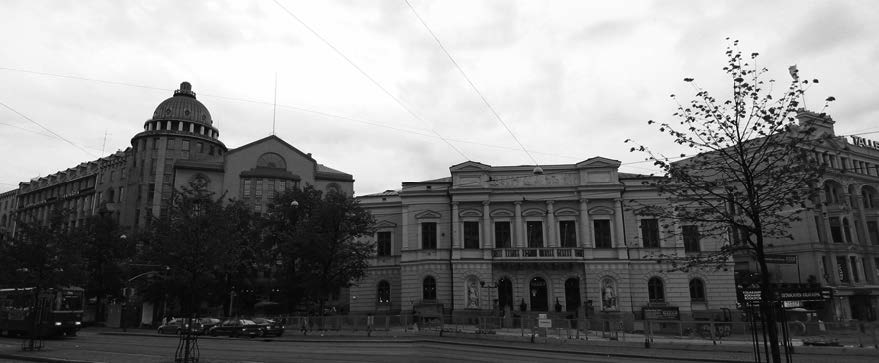
\includegraphics[width=\textwidth]{vanhajauusi.png}
\end{figure*}

Ylioppilaskunnan ylin päättävä elin
on 60-henkinen edustajisto, joka valitaan
vaaleilla joka toinen syksy. Edustajisto tekee keskeisimmät päätökset sekä valitsee
toimeenpanovaltaa käyttävän hallituksen
ja keskustoimiston esimiehenä toimivan
pääsihteerin. Hallitus puolestaan nimittää
keskustoimistolla työskentelevät toimintasihteerit,
joiden vastuulla suuri osa ylioppilaskunnan
toiminnasta on. Vapaaehtoisista
HYYn jäsenistä koostuvat valiokunnat
puolestaan tarjoavat mahdollisuuden osallistua
ylioppilaskunnan toimintaan joutumatta
sotkeutumaan opiskelijapolitiikan
kiemuroihin.
\subsection*{Ylioppilastaloja}
Odottavan aika on pitkä, sanotaan, ja
niin se on ollut. Ylioppilastalo rakennettiin
vuonna~1868, se jäi nopeasti pieneksi
ja sen viereen rakennettiin Uusi ylioppilastalo
vuonna~1910, eli yli sata vuotta sitten!
Aikojen saatossa tilat ovat jääneet pieniksi
ja epätarkoituksenmukaisiksi, eikä niiden
jako eri käyttötarkoituksiin vastaa sekään
enää tämän päivän tarpeita.
Pitkä odotus kuitenkin palkittiin kolmannen
ylioppilastalon valmistuttua Leppäsuonkadulle
Kamppiin. Matlulaiset
järjestöt (kaikki Kumpulan ja kaksi Viikin,
mm.\,Limes ja yhden aineen järjestöt)
muuttivat vuoden~2009 alussa yhteiseen kerhotilaan,
eli Klusteriin. Nimitys Klusteri on jo käytännössä vakiintunut, vaikka koekäytössä
on ollut myös muita nimiä, mm.\,Leppäkertsi
ja Ilotalo.

\vspace{0.5cm}\noindent
\textsc{Jouni Siren}\\
\textsc{Jaana Saarni}\\
\textsc{Daniel Landau}

\twocolumn[\section{Ammattiliitot}]
\subsection*{Lyhyesti: Järjestyminen}
Ammattiliitto on helposti sanottuna
yhdistys, joka neuvottelee työntekijöiden
puolesta palkankorotuksista ja lomista sekä
huolehtii, että sopimuksia noudatetaan ja
töitä riittää myös tulevaisuudessa.

Luonnon-, ympäristö- ja metsä\-tieteilijöiden liitto Loimu ja Tekniikan akateemisten liitto
TEK ovat sinun Akavalaisia ammattiliittojasi.
Akava on se iso järjestö, joka vaikuttaa
eduskuntaan ja vetää isoja linjoja. Liittosi
edustaja on se joka auttaa sinua henkilökohtaisesti,
kun sinulle tulee kysyttävää
työelämästä tai pahimmassa tapauksessa
ongelmia työnantajan kanssa. Kun kuulut
liittoon, et ole koskaan yksin työelämässä.

Ammattiliitto hoitaa asioitasi kahdella
tasolla: kollektiivisesti ja henkilökohtaisesti.
Kollektiivisesta edunvalvonnasta
hyötyvät kaikki, siis myös ne, jotka eivät
itse kuulu mihinkään ammattiliittoon. Kollektiivisia
etuja ovat työehtosopimuksista
neuvotteleminen ja alan näkyvyydestä huolehtiminen.
Mitä enemmän meillä on jäseniä
sitä parempia sopimuksia ja etuuksia
voimme neuvotella. Järjestäytymättömät
nauttivat usein järjestäytyneiden tekemästä
työstä mm.\,palkankorotusten eteen, mutta
todellisuudessa he syövät kuormasta.

Henkilökohtaiset edut tietenkin koskevat
vain jäsenmaksun maksaneita. Tällaisia
ovat esimerkiksi työhakemuksen ja CV:n
kommentointi, erilaiset koulutukset, juristin
apu ongelmatilanteissa ja työttömyysturva.

Jos haluat tietää mihin tutkinnollasi
työllistyy, mitä työelämä tuo tullessaan tai
yleensäkin mitä alalla tapahtuu, me tiedämme
vastaukset näihin ja moniin muihin kysymyksiin.

Korkeasti koulutetut järjestäytyvät Suomessa
liittoihin koulutusalansa mukaan,
joten jokaisella liitolla on paras osaaminen
juuri oman alansa asioissa. Ensiarvoisen
tärkeää on esimerkiksi alalle koulutettavien
määrän suhteuttaminen niin, että ne vastaavat
yksilön, työelämän ja yhteiskunnan
tarpeita. Suomalainen kilpailukyky ja hyvinvointi
ovat koulutuksen ja tutkimuksen
korkean laadun varassa. Akavalaisten liittojen
lähtökohtana on, että koulutus kannattaa
aina!

\vspace{0.5cm}\noindent\textsc{Markus Oja}\\
\textsc{Laura Koskinen}

\clearpage
\begin{figure}[h!]
	
\includegraphics[width=\columnwidth]{4500-LOIMU_log_tekstill_nega.eps}
\end{figure}
Luonnon-, ympäristö- ja metsätieteilijöiden liitto Loimu on monialainen liitto: koulutukseltaan jäsenet ovat biologeja, biotieteilijöitä, kemistejä, geologeja, limnologeja, metsänhoitajia, ympäristötieteilijöitä, meteorologeja, maantieteilijöitä, tilastotieteilijöitä, fyysikoita, matemaatikoita -- ja monia muita.

\url{www.loimu.fi}
\newpage
\begin{figure}[h!]
	
\includegraphics[width=\columnwidth]{tek_logo.png}
\end{figure}
Tekniikan Akateemisten Liitto TEK on
diplomi-insinöörien ja vastaavan yliopistokoulutuksen
saaneiden ammattiliitto, jonka
tavoitteena on edistää tekniikkaa ihmisen,
elinympäristön ja yhteiskunnan parhaaksi.
Jäsenistöömme kuuluu esimerkiksi tietojenkäsittelytieteestä
valmistuneita.

\url{www.tek.fi}

\twocolumn[\section{Työelämä -- tulevaisuuden utopiaa?}]
Onnittelut opiskelupaikasta! Edessäsi
on hieno elämänvaihe: saat oppia uusia
asioita päivittäin, tutustut mahtaviin opiskelukavereihin
ja pääset osaksi yliopistoyhteisöä.
Kuitenkin, ennen kuin ehdit edes
huomata, valmistut kandidaatiksi ja sitten
maisteriksi. Samalla opiskelukavereistasi
on muodostunut luultavasti elinikäinen ystäväpiiri
ja kattava verkosto alasi ammattilaisia.

Suunnitteletko tekeväsi jotain töitä kesäisin
tai henkesi pitimiksi lukukausien aikana?
Työmarkkina-asioille kannattaa siis
lotkautella korviaan jo opiskeluaikana.
\subsection*{Miten niitä kesätöitä löytää?}
Työnhakuun voi suhtautua niin kuin
mihin tahansa haasteeseen: miten ja mistä
löydän töitä, miten niitä haen ja mitkä
minun oikeuteni työntekijänä ovat? Tietoa
ja tukea löytyy oman oppiaineesi työelämäopinnoista,
Helsingin yliopiston Urapalveluista,
ammattiliitoista sekä monilta
verkkosivuilta!

Työnhaku vaatii aikaa, energiaa ja pitkää
pinnaa.
\subsection*{Työnhaun vaiheet}
\begin{enumerate}
	\item \textbf{Hakupäätös ja yhteydenotto
	työnantajaan}.
	Valitse avoimista hakemuksista tai mahdollisista
	työpaikoista ne, joihin haluat hakea.
	Ota yhteyttä työnantajaan reippaalla ja
	hyvin suunnitellulla puhelulla. Puhelussa on hyvä esitellä itsesi selkeästi ja ytimekkäästi,
	osoittaa kiinnostuksesi kyseessä
	olevaa työpaikkaa kohtaan ja esittää älykkäitä
	lisäkysymyksiä. Puheluita voi harjoitella
	etukäteen vaikka kaverin kanssa!
	\item \textbf{Työnhakuasiakirjojen laatiminen
	ja lähettäminen}.
	Hakemuksen ja ansioluettelon kirjoittamiseen
	kannattaa varata riittävästi aikaa.
	Hyvä keino viilata hakemuksesta loistava
	on luetuttaa sitä kavereilla tai lähettää liittoon
	kommentoitavaksi. Lähetä työnhakuasiakirjat
	juuri siinä muodossa kuin niitä
	hakuilmoituksessa pyydetään ja oikealle
	henkilölle.
	\item \textbf{Hakuprosessin seuraaminen}.
	Pidä kirjaa yhteydenotoista -- sähköposteista,
	puheluista ja lähetetyistä hakemuksista.
	Palaa asiaan 1--2 viikon kuluttua, viittaa
	aiempaan yhteydenottoon ja tiedustele,
	miltä tilanne näyttää. Yritä olla kohtelias ja
	reipas, vaikka saisitkin hylkäävän ilmoituksen.
	Saattaa nimittäin olla, että seuraavan
	paikan auetessa työnantaja muistaa sen
	hyvän tyypin ja saatkin kutsun haastatteluun!
\end{enumerate} 
Muistilista kesätöihin:
\begin{itemize}
	\item Tee työsopimus kirjallisesti kahtena
kappaleena
\item Tarkista mahdollinen työ\-ehto\-sopimus
\item Ylitöiden tekemisestä sovitaan yhteisesti
\item Palkka ja työaika työssä\-olo\-ehtoa kerryttävää
\item Liity liittoon ja työttömyys\-kassaan
\end{itemize}
En minä jää koskaan työttömäksi!
Harvalla alalla on Suomessa täystyöllisyys.
Valmistumisen jälkeinen vuosi on
todennäköisin aika olla hetken aikaa työttömänä
koko työuran aikana. Myöhemminkin
uralla kuka tahansa voi jäädä työttömäksi
tai lomautetuksi ihan milloin vaan.
Sen takia on hyvä kuulua työttömyyskassaan.
Silloin voit valmistumisesi jälkeen
saada ansiosidonnaista työttömyyspäivärahaa,
joka on aina enemmän kuin Kelan
maksama peruspäiväraha.

Opiskeluaikana voit siis jo kerryttää täyteen
ansiosidonnaiseen vaadittavan työssäoloehdon.
Se tarkoittaa yhteensä 26~viikon
työskentelyä työttömyyskassajäsenyysaikana.
Työn ei tarvitse olla oman alan töitä,
eikä tarvitse olla yhteen putkeen, vaan voit
kerryttää sen vaikka viikko viikolta. Ehdot
ovat: työtä vähintään 18 h/vko, ja palkka
jonkin työehtosopimuksen mukainen
tai vähintään 1~189~\euro/kk kokopäivätyöstä
(vuonna 2018).
\subsection*{Mitä kannattaa opiskella, jotta työllistyn hyvin?}
Kemisti, fyysikko, tähtitieteilijä, matemaatikko
jne. Mutta mitä he tekevät työelämässä?
Kuten kaikki jossain vaiheessa
opintojaan ymmärtävät, luonnontieteilijän
tutkinnolla ei työllistytä samalla tavalla
selkeästi yksiselitteiseen tehtävään kuten
vaikkapa putkimiehen tutkinnolla.

Ensimmäinen asia, joka opiskelijan tulee
hahmottaa, on vaihtoehtojen lukumäärä.
Ei ole vain yhtä tai kahta juttua jota filosofian
maisterin papereilla voi tehdä. FM
takaa työnantajalle sen, että olet kykenevä
oppimaan mitä tahansa mitä tulevassa työssäsi
saatetaan vaatia, osaat hankkia tietoa ja
ennen kaikkea, että todella ymmärrät omaa
alaasi ja sen erityispiirteitä.

Tieto on tärkeintä, kun suunnittelet
omaa uraasi. Yliopistossa ympärilläsi pyörii
professoreja ja akatemiatutkijoita, jotka
tuntuvat tietävän kaikesta kaiken ja ovat
innostuneita kertomaan tutkimuksestaan.
Voi alkaa tuntua siltä, ettei oikeastaan osaa
mitään ja edessä siintää ainoastaan tutkijan
ura apurahahakemuksineen.

Kun pysähdyt miettimään asiaa, on täysin
luonnollista, että opettajina ja ohjaajina
yliopistoissa toimivat ne jotka tietävät eniten.
Yliopistoissa opetellaan nimenomaan
asian ymmärtämistä, jolle kaikki pohjaa.
Tärkeää on hahmottaa, että yliopiston ulkopuolelle
siirryttäessä tilanne on toisinpäin.
Maisterina tiedät todennäköisesti enemmän
omasta alastasi kuin moni muu ja löydät itsesi
siitä asemasta, jossa proffat ja akatemiatutkijat
ovat yliopistolla.

Tutkija on yksi mahdollinen tehtävä mutta sen lisäksi luonnontieteilijät löytävät
itsensä muun muassa seuraavien nimikkeiden
alta; asiantuntija, laadunvalvontapäällikkö,
opettaja, avainasiakaspäällikkö,
erityisasiantuntija, henkilöstöjohtaja, informaatikko,
kehitysinsinööri, markkinointijohtaja,
tuotantokemisti, tarkastaja ja toimitusjohtaja.

Kuten huomaamme tehtäväkenttää ja
tehtäviä löytyy monenlaisia. Yhteiseksi
piirteeksi voidaan sanoa, että tehtävissä sovelletaan
oman alan osaamista. Haasteena
on saada selvää siitä mitä eri tehtävät pitävät
sisällään ja minkälaista osaamista niissä
tarvitaan, jotta voisit suunnitella opintojasi
tulevaa uraasi varten. Tähän kysymykseen
voit etsiä vastausta excursioilta, kesätöistä,
työelämätapahtumista, harjoittelusta, liitostasi,
kavereilta ja tutuilta sekä tietenkin
seuraamalla alan lehtiä. Voit kuitenkin olla
varma, että tutkintosi jälkeen olet pätevä
oppimaan minkä tahansa oman alan tehtäväsi
ja toisin kuin putkimies voit vaihtaa
uraasi tehtävästä toiseen ja tehdä monia erilaisia
tehtäviä urasi aikana.

Luonnontieteissä on mahdollisuuksia
ja sinä, onnekas, olet juuri tarttunut niihin.
Tervetuloa luonnontieteilijöiden joukkoon.

\vspace{0.5cm}\noindent
\textsc{Markus Oja}\\
\textsc{Laura Koskinen}

\twocolumn[\section{Limes}  {\small \itshape ``Matemaattis-luonnontieteellinen salaliitto järjestäytyneessä Yliopistomaailmassa'' }\vspace{0.5cm}]
Kuultu eräiden Limeksen bileiden tupakka\-paikalla:
\begin{quotation}
\noindent---Mikä ihme se Limes oikein on?\\
---Se on sellainen kirjakustantamo.\\
---Ai jaa, no miks se sit järkkää bileitä?\\
---No kato se on niinku erikoistunu Yliopiston
kirjoihin.
\end{quotation}
Onhan tuossa tietysti hitunen vääristynyttä
totuuttakin, mutta jotta osaisit vastata
kysymykseen hieman tarkemmin, niin
ohessa lyhykäinen esittely.

\begin{figure}[!b]
	
\includegraphics[width=\columnwidth]{isolimeslogo.png}
\end{figure}
Limes on perinteikäs vuonna 1936 perustettu
eksaktien luonnontieteiden ainejärjestö.
Jos siis opiskelet matematiikkaa,
tilastotiedettä, fysikaalisia tieteitä, kemiaa,
geologiaa, maantiedettä tai tietojenkäsittelytiedettä,
eli siis mitä tahansa Kumpulassa,
on Limes sinun ainejärjestösi.
Limes järjestää kulttuuri-, urheilu- ja
biletapahtumia jäsenilleen ja tarvittaessa
edustaa jäsentensä etuja yliopiston
hallinnossa ja HYYssä tapahtuvissa
asioissa. Limes on painanut kirjoja
sekä omaa ja muiden opiskelijajärjestöjen
lehtiä, mutta kesällä 2007 paino
joutui lopettamaan toimintansa ministerien
saatua päähänsä, ettei suomenkielisten
yliopisto-oppikirjojen
tuotantotoiminnan tukea tarvitse jatkaa.
Limes jatkaa kuitenkin kirjojen
kustannustoimintaa. Limes tuottaa matematiikan,
kemian ja fysiikan oppikirjoja.
Limes tukee useita alaisuudessaan toimivia
kerhoja, jotka keskittyvät mitä erilaisimpiin
harrastuksiin.
\subsection*{Etujärjestö}
Opiskelu sujuu joutuvammin, kun tarjotaan
apua ja välineitä. Limes on jo pitkään
pyrkinyt edistämään jäsentensä opiskelu\-olo\-suhteita
mm.\,aloittamalla tiede\-kunnan
tuutorointi\-toiminnan ja monistamalla kurssi\-materiaalia.
Yliopiston kehittyminen on
ollut Limeksen asia\-listalla ja olemme osallistuneet
niin hallinnon- kuin tutkinnon\-uudistustenkin
toteuttamiseen.
\subsection*{Kerhot}
Lukuisat eri harrastusmuotoja harjoittavat kerhot lisäävät vaihtelua Limesläisten
elämään. Limes tarjoaa
kerhoille kokoontumismahdollisuuden kerhohuoneellaan
ja tukee harkinnan mukaan
esimerkiksi pelivälineiden hankintaa.

Kerhojen määrä vaihtelee kulloinkin
aktiivisten jäsenten kiinnostusten mukaan,
mutta jo pitkään toimineisiin kerhoihin
kuuluvat mm.\,elokuvakerho LiEKe, shakkikerho
LiShaKe matkailukerho LiMaKe
ja strategiapelikerho LiStraKe. Uudempiin
tulokkaisiin kuuluvat esimerkiksi Leivontakerho
LiLeKe ja Teekerho LiTKe.

Kerhoiltojen aiheet voivat vaihdella silkasta
juhlinnasta esoteeriseen estetiikkaan.
Varsinaista linjaa ei siis ole, kunhan saa
kerhon pitäjät vakuuttuneeksi aiheen mielenkiintoisuudesta,
tai tulee itse mukaan
järjestämään tapahtumaa!

Vapaa-ajan monimuotoisuus auttaa pitämään
mielen vireänä, joten ei kuin mukaan
kerhoihin. Puuttuiko oma lempiharrastuksesi?
Ei hätää. Kerro ideastasi ja ehkä
juuri sinun harrastuksestasi tulee seuraava
Limes-kerho.
\subsection*{Tapahtumat}
Vapaa-ajan toimintaan kuuluvat myös
lukuisat kerhoista riippumattomat tapahtumat.
Näihin kuuluvat tietysti bileet ja saunaillat,
mutta myös vaikkapa kulttuurin ja
sivistyksen piiriin lukeutuvat käynnit museoissa,
ravintoloissa tai elokuvissa.
\subsection*{Tiedotus}
Tärkeimmistä Limes-tapahtumista saa
tietoa sähköpostilistoilta, nettisivuilta, Limeksen
Facebook-ryhmästä ja ilmoitustauluilta.
Jos haluat tietää enemmän,
liity sähköpostilistalle \url{jasenet@limes.fi},
liity Limeksen Facebook-ryhmään tai seuraa
www-sivuja osoitteessa \url{www.limes.fi}.
\subsection*{Toimisto}
Tervetuloa asioimaan tai muuten vain
hengailemaan Limeksen toimistolle Exactumiin,
huoneeseen~C132. Seura on yleisimmin
sopivan kahjoa ja (epä)tieteellistä,
jokaiseen makuun.

Toimistolla voit muun muassa liittyä jäseneksi,
ostaa Limeksen ja muiden järjestöjen
haalarimerkkejä ja ostaa kirjoja laajasta
kirjavalikoimastamme. Lisäksi voit nauttia
toimistolla ilmaista(!) kahvia ja lukea tieteellisiä
(ja vähemmän tieteellisiä) julkaisuja
kuten esimerkiksi Tiedettä tai Cosmopolitania.
Maksuvälineinä käyvät käteisen
lisäksi Visa, Visa Electron, Mastercard ja
Maestro.

Tarjoamme myös mahdollisuutta käytettyjen
kirjojen välitykseen, eli otamme
vastaan kirjoja ja myymme niitä eteenpäin
sinun määräämälläsi hinnalla. Emme peri
välityspalkkiota, sillä kyse on puhtaasti jäsenpalvelusta.
Uskallatko astua pyhälle maallemme?
Ota haaste vastaan ja koe positiivisia yllätyksiä.
Olemme avoinna viikottain vaihtuvien
aikataulujen mukaan. Ne löydät
nettisivuiltamme, tiedotuslistalta sekä
Facebook-ryhmästä.

\subsection*{Klusteri}
Yhdessä muiden kumpulalaisten järjestöjen
kanssa jaettu Klusteri on Limeksen
toiminnan keskus. Siellä kokoonnutaan
mitä erilaisimmissa merkeissä niin harrastamaan,
oppimaan kuin vain olemaankin.
Klusteri toimii avoimien ovien periaatteella,
eli kunhan paikalla on joku avaimellinen
henkilö, olet tervetullut viettämään
vaikkapa koko yön tilassa keskustellen ja
juhlien. Mainitsimmeko jo, että Limeksen
toimihenkilöt saavat tilaan avaimen?
\subsection*{Hallitus}
Limeksen toiminnasta vastaa hallitus.
Kalenterivuodeksi kerrallaan valittava
elin on elävä läpileikkaus Limeksen
jäsenaineiden opiskelijoista. Tehokkain
tapa vaikuttaa Limeksen toiminnan kehittämiseen
on ottaa yhteys hallitukseen,
joko sähköpostilla hallituksen osoitteeseen
\url{hallitus@limes.fi}, tai ilmestymällä paikalle
johonkin hallituksen kokouksista.

\begin{figure}[!b]
	\centering
\includegraphics[width=0.8\columnwidth]{wanhalimes.png}
\end{figure}
\subsection*{Aktiiviksi?}
Opiskelun ei tarvitse olla pelkkää puurtamista.
Olennainen osa yliopistossa oloa
on myös järjestötoiminta monenmoisine
tapahtumineen! Usein kaikkein antoisinta
ei ole pelkästään mukana olo vaan se, että
saat tehdä muille hyviä hetkiä! Limes on
suuri järjestö ja tarvitseekin erilaisia ihmisiä;
toimittajia, juhlien järjestäjiä, kerhon
vetäjiä, virkailijoita sekä tietysti hallituslaisia.
Tarkemmin sanoen tarvitsemme
\mbox{SINUA}! Katso nettisivuiltamme, millaista
toimintaa järjestämme ja ota yhteyttä toimijoihimme!

Limeksen nettisivuilta löytyy aina ajankohtaisin
tietopläjäys. Tapahtumakalenterista
löydät kaikki tapahtumat hallituksen
kokouksista aina muidenkin järjestöjen
pippaloihin! Ainutlaatuisen kuvablogin
kautta voit jakaa kaikkien limesläisten
kanssa vappuhörhöilysi tai kuvan kissanpennustasi.
Sivuilta löytyy myös tietoa
vuokrattavista bilekamoista sekä myytävistä
kirjoista. Stay tuned, pinnan alla
kuplii ja lisää on luvassa kokoajan!

\twocolumn[\section{LiXXKe} {\small \itshape ``Limeksen kerhot on tapana nimetä tyyliin: Li+XX+Ke, missä XX:ksi valitaan sopiva kerhon etuliite. Kuitenkin matkailukerho kirjoitetaan vain	Limake, koska se on mitä poikkeuksellisin kerho!''}\vspace{0.5cm}]
Tässä osiossa esittelemme muutaman
Limeksen legendaarisimman kerhon. Kerhojen
toiminnan aktiivisuus vaihtelee paljonkin:
pitkän unien jälkeen jokin kerho
saattaa alkaa kukoistaa, ja joku puolestaan
painua unholaan\dots Uuden kerhon voi perustaa
kuka vain Limeksen jäsen. Joko sinä
olet keksinyt oman kerhosi?
\subsection*{LiKe}
Limeksen kerhostahan tämäkin lähtöisin\dots
tunnetaan nykyään Otavan alaisuudessa
tällä nimellä. Tosin perustajia tavoittaa
enemmän Rosebud Books "-nimisestä
yrityksestä.

(Selvennyksenä: Tämä on historiaa,
mutta mukava tietää)
\begin{figure}[h!]
	\centering
	
\includegraphics[width=0.8\columnwidth]{lieke.png}
\end{figure}
\subsection*{LiEKe}
LiEKe eli Limeksen elokuvakerho jatkaa
jo 60-luvulta alkanutta Limeksen elokuvailtatraditiota.
16~mm projektori on tosin
vaihtunut videotykkiin ja DVD-levyihin,
mutta alkuperäinen idea elää: mainstream
jätetään enimmäkseen toisille tahoille ja
keskitytään lähinnä vähemmän tunnettuihin
klassikoihin koti-, lähi- ja kaukomailta
sekä uusiin, lupaaviin tekijöihin. Osallistumalla
toimintaan voit kyllä vaikuttaa ohjelmistoon
paljonkin, LiEKe kaipaa uusia
leffafriikkejä! Leffaillat järjestetään yleensä
Klusterilla, niitä on harvakseltaan ja ne
ovat ilmaisia ja avoimia Limeksen jäsenille.

\begin{figure}[h!]
	\centering
	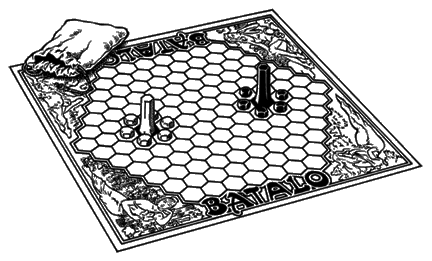
\includegraphics[width=0.8\columnwidth]{listrake.png}
\end{figure}
\subsection*{LiStraKe}
Limeksen strategiapelikerhossa
pelataan erilaisia lauta-,
kortti- ja strategiapelejä. Käytännössä
skaala kulkee varttitunnin korttipeleistä
kuukausia kestäviin sotapeleihin. Lisäksi
LiStraKe järjestää myös elektronisia strategiapelejä,
esimerkiksi Alpha Centauri "-sähkö\-posti\-pelejä.
Peli-iltoja järjestetään satunnaisesti
Klusterilla. Peli-illat ovat aloittelijaystävällisiä,
usein pelataankin pelejä, joista kenelläkään
ei ole pelikokemusta! Peli-illoissa
on usein myös tarjolla pientä purtavaa sekä
juotavaa. Peli-illoista tiedotetaan Limeksen
sähköpostilistalla, Facebookissa sekä nettisivuilla
kalenterissa!

\begin{figure}[h!]
	\centering
	
\includegraphics[width=0.8\columnwidth]{lipuke.png}
\end{figure}
\subsection*{LiPuKe}
Tämä 2000-luvun alusta toiminut Limeksen
pullokerho kokoontuu säännöllisen
epäsäännöllisesti arvioimaan pullojen
sisältöä sekä taltioimaan etiketit arvioineen
tulevia sukupolvia varten. Kerhon kantavana
ideana on tuoda arvioitavaksi pullo,
jonka etikettiä ei kokoelmista vielä löydy.
Samainen kriteeri toimii myös jäsenanomuksena
lisänä euron liittymismaksu.
Nämä kokoukset ovat kuivasta kaukana
mutta aikaa kannattaa varata riittävästi,
sillä arvioiminen voi jatkua pitkälle yöhön
(lue: Koet aamun ensimmäiset auringonsäteet
Klusterin sohvalta katsottuna\dots).

\begin{figure}[h!]
	\centering
	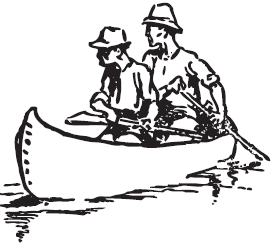
\includegraphics[width=0.8\columnwidth]{limake.png}
\end{figure}
\subsection*{LiMaKe}
Opiskelumatkailua ja typeriä ideoita jo
vuodesta 1988!

Haluatko nähdä maailmaa? Kaipaatko
tuttua matkaseuraa? Eivätkö perinteiset
seuramatkat kiinnosta, mutta et myöskään
jaksa itse huolehtia matkajärjestelyistä?
Haluatko matkustaa jonnekin, minne et
omin päin tulisi ikinä lähteneeksi? Jos vastauksesi
johonkin näistä kysymyksistä on
kyllä, saattaa Limeksen matkailukerho olla
juuri sinua varten.

Limakkeen alkuajat esihistoriallisella
80-luvulla ovat nyt jo kadonnutta kansanperinnettä.
Muinaisella 90-luvulla
matkoja saattoi olla useita vuodessa, ja
ne suuntautuivat yleensä jonnekin päin
Eurooppaa. Sen jälkeen koitti muutaman
vuoden hiljaisempi jakso, kunnes uudet
ihmiset herättivät kerhon jälleen henkiin.
Limakkeen tavaramerkkinä ovat useiden
viikkojen matkat jonnekin kauas -- toki
puolimatkassakin saa jäädä pois tai liittyä;
keväällä 2006 vietettiin kolme viikkoa
Kiinassa ja viimeisimpänä keväällä 2007
laajempi itäkierros, joka vei junalla halki
Aasian. Osalle tämäkään ei vielä riittänyt,
vaan seikkailu johti Tiibettiin, Nepaliin ja
lopuksi Intian kautta takaisin Suomeen.
Vuonna 2011 suunnattiin Moskovan kautta
Kiovaan, sieltä Tsernobyliin ja lopulta osa
porukasta päätyi Krimille Kazantip-festivaaleille.
Kaukomatkailu saattaa vaikuttaa
kalliilta, mutta ei välttämättä ole sitä.

Mitä kauemmas länsimaista menee, sitä
halvemmaksi eläminen yleensä muuttuu.
Talkootöitä tekemällä, bileitä järjestämällä
ja tv-ohjelmissa studio\-yleisönä vierailemalla
saattaa rahoittaa suuren osan matkastaan,
eikä ole aivan mahdotonta, että joku
sponsorikin erehtyisi osallistumaan matkan
kustannuksiin.

Uusia matkoja ei tällä hetkellä ole kiikarissa,
mutta kukapa tietää, ehkä jo huomenna
joku jossain kokoaa porukkaa matkaseuraksi
juhannuksen viettoon Tongalle?

Muista myös nämä: Ponikerho LiPoKe,
Halvan kaljan kerho LiHaKaKe, Hasselhoff-kerho LiHaKe, Pöydällä tanssimis- ja
musiikin\-kuuntelu\-kerho LiPöTaMuKuKe,
Särkyneiden sydämien kerho LiSäSyKe.

% ainejärjestöjä
\twocolumn[\section{Matrix}]
Matrix on sinun ja muiden matikan
opiskelijoiden ainejärjestö. Tarjoamme
mahdollisuuden jakaa matematiikan lukuisat
ahaa-elämykset muiden opiskelijoiden
kanssa järjestämällä niin vapaa-ajan
kuin itse opiskeluunkin liittyvää toimintaa.
Ekskursioita, marsseja ja näiden välissä
kaikkea mitä me kaikki yhdessä vain päissämme
keksimme, oli se sitten saunomista,
bilettämistä tai lintujen tähystelyä. Pelkkää
hupia ei kuitenkaan toimintamme ole, sillä
valvomme myös aktiivisesti etujasi niin
yleisesti kuin erityisesti juuri matematiikan
opiskelijana.

Matrix perustettiin 1.3.1995 joten olemme
lähes kolmikymppinen ainejärjestö. Matrixin
koti on Exactumin kolmannessa kerroksessa sijaitseva
opiskelijahuone Komero (huone~C338).
Nimi juontaa juurensa oppiaineen vanhaan
sijaintiin Heimolan talossa, missä opiskelijoiden
taukokäyttöön annettiin, alun perin
mitä todennäköisimmin siivouskomeroksi
suunniteltu, parin neliön piskuinen kaappi.
Exactumin Komero on kuitenkin tilava ja
viihtyisä tila, missä voi huoahtaa päivän
kiireiltä -- nauttia kupposen kahvia ja rupatella
kavereiden kanssa. Laskarivinkkejäkin
voi kalastella, jos siltä tuntuu.

Kotimme etäpiste, muiden ma\-te\-maat\-tis-luon\-non\-tie\-teel\-lis\-ten järjestöjen kanssa jaettu Klusteri, löytyy puolestaan Domus
Gaudiumista (``kolmas yli\-oppilas\-talo'' Leppä\-suon\-kadulla).
Tulemalla mukaan toimintaan
on jokaisella mahdollisuus muokata
Matrixia oman\-näköisekseen. Innokas virkailija\-joukkomme
lähtee mielellään toteuttamaan
mitä ihmeellisempiäkin ideoita.

\noindent URL:\\\url{https://wiki.helsinki.fi/display/Matrix/Matrix+ry}

\noindent e-mail: \url{matrix-ry@helsinki.fi}

\begin{figure}[!b]
	\centering
	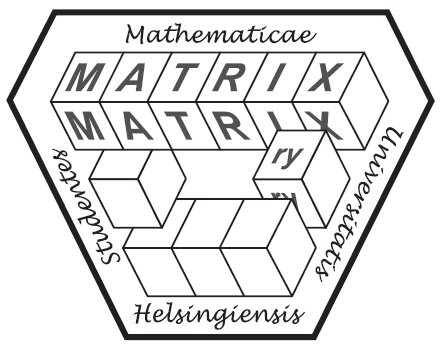
\includegraphics[width=0.9\columnwidth]{matrix.png}
\end{figure}

\twocolumn[\section{Resonanssi}]
Jo yli kahden vuosikymmenen ajan Resonanssi~ry, Helsingin yliopiston fysikaalisten
tieteiden oma ainejärjestö, on tarjonnut
jäsenilleen virkistävää vastapainoa opintojen
kanssa puurtamiselle ja huolehtinut
fysiikanopiskelijoiden eduista yliopistolla.

Järjestämme jäsentemme iloksi sekä
saunailtoja ja bileitä että yritys- ja kulttuuriexcuja.
Kesällä toiminta keskittyy monipuoliseen
liikuntaan kuten jalkapalloon, ultimateen
ja pesäpalloon. Resonanssilla on
myös kerhoja, kuten elektroniikka-kerho
ELKE, lautapelikerho, ompelukerho ja Hullujen
ideoiden toimikunta HIT.

Päämajanamme toimii Physicumin pohjakerroksessa
Unicafen takana sijaitseva
opiskelijahuone. Sieltä löydät tieteen eturintaman
julkaisut (Helsingin Sanomat ja
Aku Ankka). Voit myös mm.\,pelata shakkia,
gota, korttia, Settlers of Catania, Carcassonnea,
lukea sähköpostisi, syödä pehmistä
tai muuten vaan nauttia mukavasta
seurasta. Kannattaa uskaltautua kynnyksen
yli, sillä moni on tullut ennen sinua ja moni
tulee sinun jälkeesikin. Tervetuloa!

Resonanssiin liittyminen onnistuu alkusyksystä
Physicumin aulassa pidettävässä
fuksipäivystyksessä, tai sitten koska
tahansa tulemalla opiskelijahuoneelle ja
ilmoittamalla liittymishalustaan jollekin
hallituksen jäsenelle. Liittymismaksu on
2~euroa (sisältää haalarimerkin, ensimmäisen
vuoden jäsenmaksun ja kupin kahvia
tai teetä) ja lukuvuosittainen jäsenmaksu 1~euro.

Kansainvälisyydestä kiinnostuneille on
luvassa toimintaa Suomen fysiikan- ja matematiikan\-opiskelijat
ry:n kautta. Joka kesä järjestetään
kansainvälinen fysiikanopiskelijoiden konferenssi
ICPS jossain päin maailmaa. Joka
vuosi syksyllä pidettävä Fysikerfest kerää
myös paljon osallistujia.

Resonanssi ilmoittelee toiminnastaan
sähkö\-posti\-listallaan \url{reson@helsinki.fi},
www-sivujen tapahtuma\-kalenterissa ja isoa
luento\-salia vasta\-päätä olevalla ilmoitus\-taululla.
Parhaiten pysyt kuitenkin ajan tasalla
tulemalla hallituksen kokouksiin, jonne
kaikki jäsenet ovat tervetulleita.

\noindent URL: \url{www.resonanssi.org}

\noindent e-mail: \url{reson-ry@helsinki.fi}

\begin{figure}[!b]
	\centering
	
\includegraphics[width=0.9\columnwidth]{resonanssi.png}
\end{figure}

\twocolumn[\section{Moodi}]
Hei ystävät, ja merkitsevästi tervetuloa myös Moodin puolesta yliopistoon ja Kumpulaan! Tilastotieteen opiskelijoiden yhteinen Moodi~ry on yksi harvoista useamman tiedekunnan ainejärjestöistä. 50~vuoden kiitettävään ikään varttuneen järjestömme matkassa voi siis vahingossa tutustua muihinkin kuin tilastotieteen opiskelijoihin. Kaikkein parasta Moodissa on, että kerran paikalle päätynyt myös odotusarvoisesti muistetaan jatkossa, ja mukaan on helppo lähteä kenen tahansa -- oli tarkoituksena sitten opiskella tilastotiedettä kurssin verran tai tehdä siitä itselleen tulevaisuus.

Aktiivista kerhotoimintaamme edustavat muun muassa MoPPI ja \\MoPSi -- eli Moodin pöytäpeli-ilta ja Moodin palloseura, jotka eivät jätä kovintakaan peluria kylmäksi. Perinteikäs seuramme on aiheuttanut silkkaa kauhua vastustajien kasvoille erinäisissä otteluissa. Tiukan pelailun ohessa on hyvä muistaa välillä myös rentoutua. Tästä pitää huolen Moodin kattava tapahtumatarjonta. Perinteeksi ovat muodostuneet pikkujoulut, kesäpiknik, toisinaan järjestettävät ulkomaanreissut sekä tietenkin helmikuussa järjestettävät syntymäpäiväsitsit. Vaihtelevia tapahtumia muiden järjestöjen kanssa niin Kumpulasta, valtsikasta kuin näiden ulkopuoleltakin riittää yllin kyllin koko vuoden ympäri.

Tapahtumien ja kerhotoiminnan ohessa Moodilla on myös vakaa ote opintoasioista. Lisäksi olemme yhteydessä virallisempiin tahoihin, kuten Tilastokeskukseen, ja myös esimerkiksi pankit saattavat joskus saada tiloihinsa tilastojoukon iloisen.

Tervetuloa siis mukaan joukkoon! Alun innostusta voit helpottaa klikkaamalla itsesi Facebook-sivuillemme (Moodi~ry), Instagram-tilillemme (\texttt{@moodi\_ry}) tai kotisivuillemme (\url{https://blogs.helsinki.fi/moodi-ry/}). Plärää myös läpi palkittua Tyyppiarvo-lehteämme (\url{http://tyyppiarvo.com}), jonka juttuja on päätynyt aina Helsingin Sanomiin asti. Kampukselta bongaat moodilaista seuraa käytännössä aamusta iltaan opiskelijahuoneestamme Survomosta, joka sijaitsee Exactumin kellarikerroksessa Unicafen vieressä. Tarjolla on kahvia ja seuraa niin ajan kuluttamiseen, päiväuniin kuin laskareiden pähkäilyyn.

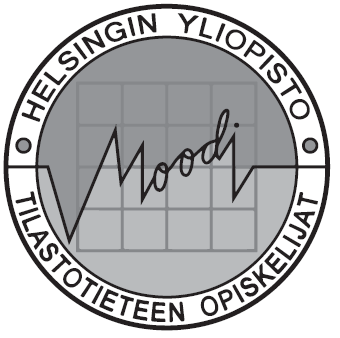
\includegraphics[width=\columnwidth]{moodi.png}	

\twocolumn[\section{Helsingin yliopiston kemistit (HYK)}]
Helsingin Yliopiston Kemistit ry (HYK)
on kemian opiskelijoiden ainejärjestö, jolla
on yli 90~vuoden perinteet. Järjestö ajaa
kemian opiskelijoiden etua koulutusohjelmissa, tiedekuntaneuvostossa
ja HYYssä sekä osallistuu aktiivisesti opetuksen kehittämiseen.

HYK järjestää jäsenilleen toimintaa bileiden,
pöytäjuhlien, saunailtojen ja peli-iltojen
sekä muiden tapahtumien merkeissä.
HYKillä on oma lauta- ja korttipelikerho
Mithril sekä elokuvakerho Bentsokinoni,
jotka järjestävät omia illanviettojaan.

HYKillä on Kumpulan Unisportissa oma liikuntavuoro
keskiviikkoisin kello~16.00. HYK järjestää myös
erilaisia ekskursioita kemian alan yrityksiin
sekä kulttuuri- ja liikuntatapahtumiin.
Tietoa toiminnasta saat Opsosin ilmoitustaululta,
Facebook-sivulta ja "-ryhmästä sekä sähköpostilistalta (\url{hyk-jasenet@helsinki.fi}),
liittymisohjeet kotisivuilla.

Kemistejä löydät varmimmin hengailutila
Opsosista (B134a) Chemicumin 1.\,kerroksesta
B-siiven välikäytävältä tietokonetilan vierestä. 
Opsosissa on mahdollista ostaa itselleen kahvia ja teetä,
pientä purtavaa, labratakkeja ja haalarimerkkejä sekä tavata useat possumme.

HYKillä on lisäksi kerhotila Domus Gaudiumissa
Leppäsuolla yhdessä muiden Matlun järjestöjen kanssa.

\noindent URL: \url{https://www.hyk.fi}

\noindent e-mail: \url{hy-kemistit@helsinki.fi}

\begin{figure}[!b]
	\centering
	
\includegraphics[width=0.8\columnwidth]{hyklogo.png}
\end{figure}

\twocolumn[\section{Geysir}]
Geysir~ry on vuoden 1997 lopulla perustettu
geofysiikan opiskelijoiden ainejärjestö,
ja näin ollen vietti juuri 20-vuotissynttäreitään! 

Geofysiikka on siitä erikoinen ala, että meillä ei ole omaa opintosuuntaa kandivaiheessa, vaan opiskelut ovat painottuneet maisterivaiheeseen. Ilmakehä\-tieteiden maisteri\-ohjelma (ATM-MP) ja Geologian ja geo\-fysiikan maisteri\-ohjelma (Geo$^2$) haravoivat opiskelijoita useista eri kandi\-ohjelmista, erityisesti fysikaalisten tieteiden ja geo\-tieteiden puolelta, mutta niihin voidaan valita myös muita geo\-fysiikasta kiinnostuneita, kunhan heillä on riittävät esitiedot ohjelmissa opiskelemiseen. Sinustakin voi siis tulla geo\-fyysikko! Geysirin jäseneksi
kannattaa liittyä jo fuksina, koska ensimmäisen
vuoden opiskelijoilta ei peritä jäsen\-maksua.

Järjestämme mahdollisimman moni\-puolista
toimintaa jäsenten toiveiden mukaan,
esimerkiksi ekskuja alan opetus- ja tutkimus\-laitoksiin,
pesäpallon peluuta, illanviettoja (leffa\-illat ja
hengailut) sekä retkiä niin kotimaahan kuin
ulkomaillekin (Islanti 2004, Viro 2005,
Huippuvuoret 2006, Uusi-Seelanti 2008,
Azorit 2012, Unkari 2014, Sisilia 2016, Kuolan niemimaa 2018). Osallistumme
myös perinteisiin opiskelija\-rientoihin laskiaisena
ja vappuna, sekä sitsaamme joko yksin tai muiden järjestöjen kanssa. Välit ovat erityisen lämpimät sisarjärjestöihin Synopiin, Vasaraan ja MaOon, joiden kanssa saunomme joka maaliskuu Geo\-saunassa.

Opiskelija\-edustajamme
huolehtivat, että sanamme kuuluu tiede\-kunta\-neuvostossa ja maisteri\-ohjelmien johto\-ryhmissä. Mikäli mieleen tulee joitakin geo\-fysiikkaan
tai aine\-järjestöömme liittyviä kysymyksiä,
Geysirin hallitus ja hall\-op\-edit vastaavat
niihin mielellään. Physicumin ensimmäisessä
kerroksessa on opiskelija\-huone, johon
olet erittäin terve\-tullut.

Vieraile toki kotisivuillamme, joilta löytyy
muun muassa liittymisohjeet ja geofysiikan
alan linkkikokoelma.

\noindent Tervetuloa mukaan!

\noindent URL: \\\url{https://blogs.helsinki.fi/geysir-ry/}

\noindent e-mail: \url{geysir-lista@helsinki.fi}

\begin{figure}[!b]
	\centering
	
\includegraphics[width=0.8\columnwidth]{geysirlogo.png}
\end{figure}

\twocolumn[\section{Maantieteen Opiskelijat (MaO)}]
MaO on vuonna 1971 perustettu yhdistys,
ja tarkoituksenamme on yhdistää ja aktivoida
jäseniämme sekä ajaa maantieteen
opiskelijoiden asiaa tiedekunnassa, yliopistolla,
ylioppilaskunnassa ja yleensä yhteiskunnassa.
MaOn jäseniksi voivat liittyä
kaikki maantiedettä lukevat opiskelijat.
Järjestämme jäsenillemme monenlaista
toimintaa bileistä urheilutoimintaan ja ulkomaille
suuntautuviin retkiin. Fukseille
järjestämme syksyisin toimintaa pääasiassa
tuutoreiden johdolla. Erityisesti fukseille
suunnattuja tapahtumia ovat esimerkiksi
fuksiaiset, fuksisitsit sekä erilaiset tuutorryhmissä
tapahtuvat toiminnot. Tuemme
myös osaltamme fuksejamme järjestämällä syksyllä opintoinfon ja keväällä
opintokokonaisuusinfon
auttamaan opintoihin liittyvissä
valinnoissa.

Tarjoamme myös kaikille jäsenillemme
suunnattuja tapahtumia, joihin lukeutuvat
muun muassa alue\-tieteen sekä luonnon\-maan\-tieteen
retket, erilaiset urheilu\-toiminnat,
bileet sekä usein vuoden kohokohtana
nähdyn kulttuuri\-maan\-tieteen retken johonkin
Suomen läh\-alueen maahan. Järjestämme
myös Kumpulassa perinteeksi
muodostuneet käytävä\-vohvelit kaksi kertaa
vuodessa.

Ylläpidämme suhteita muihin ainejärjestöihin
ja opiskelijoihin erilaisten yhteistapahtumien
muodossa. MaOn kautta
pääset siis kosketuksiin paitsi maantieteilijöiden
myös esimerkiksi Aallon maanmittareiden
sekä muiden Kumpulan ainejärjestöjen
ja opiskelijoiden kanssa.
Parhaiten meidät löytää Physicumin
ytimestä eli Valopihan sohvilta, jossa tarjoamme
jäsenillemme edullisesti kahvia
sekä teetä. Sohvilla voi kuluttaa aikaansa
lukemalla Hesaria tai maantieteilijää
kiinnostavia lehtiä.

Ainejärjestölehtenämme toimii Mantu,
joka julkaistaan 4+1 kertaa vuodessa. Lehteen
voivat kirjoittaa kaikki MaOn jäsenet,
ja lehteä voi tulla lukemaan Mantsan sohville. Tapahtumista ja ajankohtaisista
asioista tiedotamme sekä perinteisesti ilmoitustauluilla
että modernimmin Internet-sivuillamme sekä
sähköpostilistamme \url{mao-lista@helsinki.fi} kautta.

\noindent URL: \\\url{https://blogs.helsinki.fi/maantieteenopiskelijat-ry/}

\noindent e-mail: \url{mao-hallitus@helsinki.fi}

\begin{figure}[!b]
	\centering
	
\includegraphics[width=0.8\columnwidth]{maologo.png}
\end{figure}
\twocolumn[\section{TKO-äly}]
TKO-äly~ry on Helsingin yliopiston tietojen\-käsittely\-tieteen
opiskelijoiden aine\-järjestö,
joka ajaa opiskelijoiden etua opinto\-asioissa
ja järjestää moninaista vapaa-ajan
toimintaa sekä opiskelun oheis\-toimintaa.
Tärkeä osa toimintaa on myös uusien opiskelijoiden
eli fuksien vastaan\-ottaminen.

\begin{figure}[!b]
	\centering
	
\includegraphics[width=\columnwidth]{tkoaly.png}
\end{figure}
Meidät tavoittaa Kumpulan kampuksen
Exactum-rakennuksen opiskelija\-huoneesta
DK115 (Gurula), jossa myös tarjoamme
jäsenistöllemme oma\-kustanne\-hintaan kahvia,
limpparia ja naposteltavaa.
Toiminnastamme saat lisää tietoa näiden
sivujen lisäksi liittymällä sähkö\-posti\-listallemme.

Uusien opiskelijoiden kannattaa myös
muistaa reaali\-aikaisimmat tiedon\-lähteemme, eli fuksiryhmä
sekä yleiselle keskustelulle tarkoitettu TKO-äly~2018 "-ryhmä.

Linkit Telegram-ryhmiin ja niiden kanssa sillattuihin IRC-kanaviin
sekä paljon hyödyllistä tietoa löydät
Fuksi\-wikistämme osoitteessa \url{https://fuksiwiki.tko-aly.fi/}

\vspace{0.5cm}\noindent\textsc{Miia Rämö}

\twocolumn[\section{HAO}]
HAO eli Helsingin Aineenopettajiksi
Opiskelevat~ry on kaikkien yli\-opistossamme
aineenopettajiksi opiskelevien
ainejärjestö. Järjestömme valvoo aineen\-opettaja\-opiskelijoiden
etuja, osallistuu
opettajankoulutuksen kehittämiseen ja järjestää
monipuolista toimintaa esimerkiksi
bileiden, illanviettojen ja erilaisten excujen
muodossa. HAOn jäsentoimintaan on
helppo tulla mukaan, ja järjestössämme on
aina tilaa uusille ja ei-niin-uusille opiskelijoille.

HAO kokoaa yhteen opintojen eri
vaiheessa olevat opeopiskelijat ja mahdollistaa
näin arvokkaat kontaktit yli oppiaine- ja
tiede\-kuntarajojen. Meihin voit aina ottaa
rohkeasti yhteyttä, jos kaipaat apua, tukea,
muutoksia tai neuvoja opettajaksi opiskelemisessa.

Viiden euron muodollinen jäsen\-maksumme
oikeuttaa viiden vuoden jäsenyyteen,
joten opettajaksi tähtäävän kannattaa
liittyä jäseneksemme heti koulutukseen hyväksymisen
jälkeen! Älä erehdy luulemaan
meitä vain pedagogisten opintojesi aikaiseksi
järjestöksesi: olet tervetullut osallistumaan
toimintaamme koko opintojesi
ajan. Jäseneksi pystyt liittymään helposti
nettisivujemme lomakkeella. Jäsenyydellä
saat alennuksia mm.\,järjestämistämme
excu-, teatteri-, konsertti- ja leffakäynneistä
sekä illanvietoissamme ja kahvituksissa
tarjoilun ilmaiseksi.

SOOLiin eli Suomen Opettajaksi Opiskelevien
Liittoon liittyminen edellyttää
HAOn jäsenyyttä. SOOL tarjoaa jäsenetuina
Opettaja-lehden, matka-, tapaturma-
ja vastuuvakuutuksen sekä mahdollisuuden
liittyä työttömyyskassaan.
Kauttamme pääset ammattiliiton jäseneksi
jo opiskeluvaiheessa.

Uusi aineenopettajaksi opiskeleva, onnittelemme
sinua hienosta uravalinnastasi
ja toivotamme sinut tervetulleeksi mukaan
toimintaamme!

\noindent URL: \\\url{https://blogs.helsinki.fi/hao-ry/}

\noindent e-mail: \url{hao-ry@helsinki.fi}

\begin{figure}[!b]
	\centering
	
\includegraphics[width=0.8\columnwidth]{haologo.png}
\end{figure}

\twocolumn[\section{Spektrum} {\small \itshape ``Spektrum -- ainejärjestö sinulle, joka osaat ruotsia''\\
``Spektrum -- ainejärjestö sinulle, joka et (vielä) osaa ruotsia''\\
``Spektrum -- ainejärjestö sinulle, joka pidät hauskanpidosta''}\vspace{0.5cm}]
\subsection*{Mitä jos ruåtsiks? Att liksom på svenska!}
Alltså, liksom, mikäli haluat osaksi hieman
erilaista, pientä, mutta sitäkin aktiivisempaa
yhteisöä sinun kannattaa ehdottomasti
hakeutua Exactumissa sijaitsevaan
kahvihuoneeseemme (C127). Kuuntele
tarkasti, niin kuulet puheensorinaa toisella
kotimaisella ja löydät varmasti perille.
Vaihtoehtoisesti voit nettisivujen ja sähköpostilistan
avustuksella yrittää eksyä
Kirkkokadulle Klubbenille, siellä spekkarit
kokoontuvat enemmän tai vähemmän
säännöllisesti pitämään hauskaa. Takaan
ettet tule katumaan, jos ei ruotsin kieli vielä
taivu niin sen oppii erittäin nopeasti vaaleanpunaisten
haalareiden iloisessa seurassa.
Jätte bra!

Spektrum on ruotsinkielinen matematiikan,
fysiikan, kemian ja tietojenkäsittelytieteiden
ainejärjestö. Ensi silmäyksellä
voimme vaikuttaa hieman ruotsinkieliseltä
Limekseltä, mutta tämä on kaukana totuudesta.
Spektrum on kemistien perustama
vuonna 1933, eli siis jo ennen Limestä.
Voisi melkein sanoa että Limes on suomenkielinen
Spek\dots no ei nyt sentään!

Mutta jos siis haluat pitää hauskaa ruotsiksi
pienessä, mutta sitäkin aktiivisemmassa
porukassa olet tervetullut Spektrumiin.
Kannattaa myös tutustua ruotsinkielisiin
kursseihin, joskus pienemmissä ryhmissä,
uusien ihmisten kanssa voi olla palkitsevampaa
opiskella.

\begin{figure}[!b]
	\centering
	
\includegraphics[width=\columnwidth]{spektrum.png}
\end{figure}

Nyt sitten asiaan: Om du är svensk\-språkig
och vill fort\-sätta studera matta, fyssa
eller kemma på svenska så har du tur! En
svenskspråkig matematiker sover några år
till ackompanjemanget av sitt moder\-smål.
Några grund\-läggande kurser ordnas nämligen
på svenska. På Physicum och Chemicum
är det ännu bättre ställt, så gott som
alla obligatoriska kurser hålls på svenska,
Dessutom har man goda möjligheter att
påverka vilka valbara kurser som hålls på
svenska. Data\-under\-visning existerar tyvärr
bara på finska, men svensk handledning
kan man få. Det bästa dock med att studera
på svenska vid Gumtäkt är naturligtvis
Spektrum!

Spektrum är din ämnesförening som
svenskspråkig studerande vid Campus
Gumtäkt. Nu följer det viktigaste rådet jag
kan ge dig, du nya studerande: Var modig
och kom med! Spektrum är inget att vara
rädd för, fast vi är en liten grupp välkomnar
vi nya människor med öppna armar (eli
siis mukaan vaan! Emme me pure vaikka
ruotsia puhummekin). För att vara en liten
förening erbjuder vi ett stort urval av aktiviteter.
Allt ifrån livliga fester och sitser på
``Klubben'' (Kyrkogatan~10), via en mängd
sportaktiviteter till spelkvällar i kafferummet
och på Klubben. Det händer sig även
att en grupp spektrumiter yrar iväg på teater
eller något annat kulturellt alltid nu och
då. Tycker man att allt detta inte räcker är
det dessutom mycket enkelt att påverka
verksamheten. Oftast krävs inte mycket
mera än ett ``Hej, tänk om vi sku\dots'' i passligt
sällskap.

Förutom allt detta kan man nämna att
allt skitsnack i stil med: ``\dots det goda med
att studera på svenska är att grupperna alltid
är små, man känner alla, kan samarbeta
bättre, får bättre kontakt med föreläsare
och assistenter\dots'' stämmer till punkt och
pricka. Andan och gemenskapen bland de
svenskspråkiga är mycket god och stark,
både på föreläsningarna i Gumtäkt och på
sitserna på Klubben. Det enda som krävs
av dig är att du kommer med, resten följer
automatiskt.

Ja päätökseksi, och avslutningsvis, lause
joka on molemmilla kotimaisilla sama,
ett uttryck som är lika på båda inhemska
språken, nimittäin, nämligen: Hyvä juttu!

\noindent URL: \url{www.spektrum.fi}

\noindent e-mail: \url{styrelse@spektrum.fi}

\vspace{0.5cm}\noindent\textsc{Fanny Bergström}

\twocolumn[\section{Meridiaani}]
Kaikki ilmakehän tällä puolen on triviaalia!
Lisäksi tähtitiede sisältää koko fysiikan.
Pieni ja notkea ainejärjestömme
peli-iltoja, grilli-iltoja ja silloin tällöin
jokusen excunkin. Viimeisen muutaman
vuoden aikana kuukausittain kokoontuva
Meridiaanin puolivirallinen olutkerho
on saavuttanut vankan suosion. Vuosittainen
kohokohtamme on legendaariset
Yuri's Night "-bileet, joita vietetään huhtikuussa
Yuri Gagarinin, ihmiskunnan
ensimmäisen, avaruuslennon kunniaksi.
\begin{figure}[!b]
	\centering
	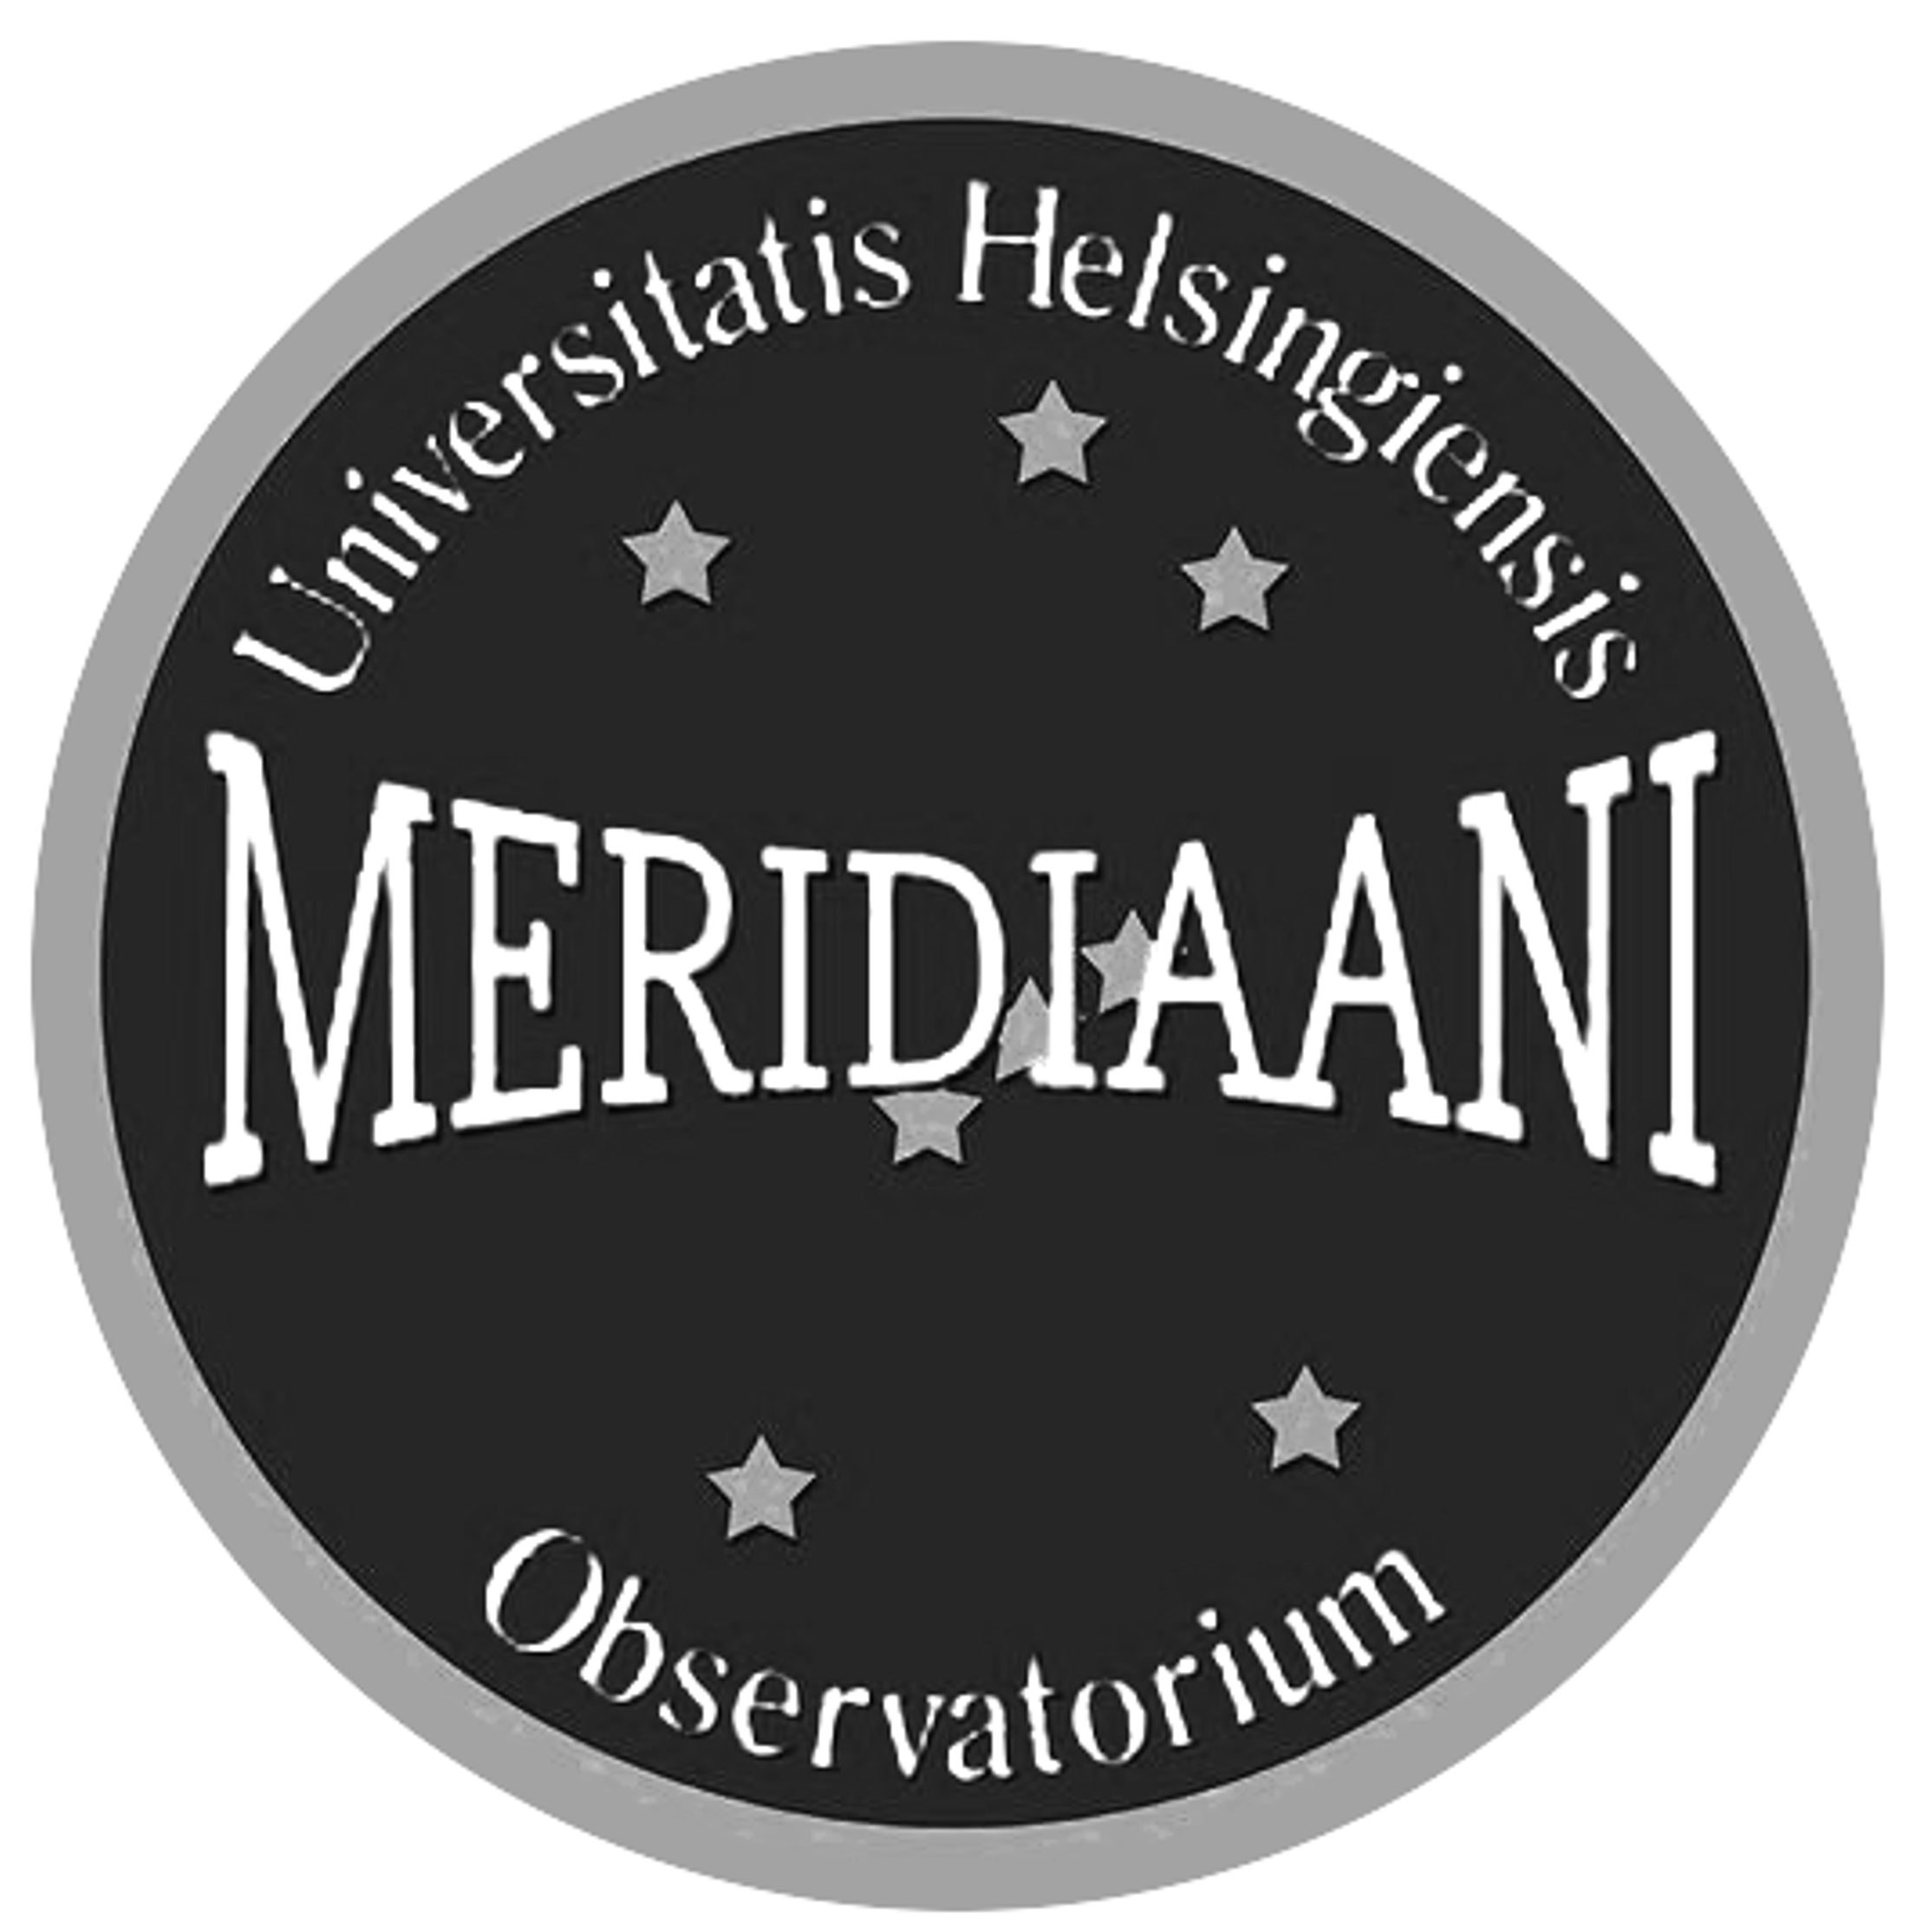
\includegraphics[width=\columnwidth]{meridiaani.png}
\end{figure}

Meridiaanilla on myös viimeisen parin
vuoden aikana hyvin aktiivisesti toiminut
Havaintoryhmä. Yliopistolla on
Kirkkonummen Metsähovissa Suomen
suurimpiin kuuluva teleskooppi, jolla
Havaintoryhmä käy kuvaamassa lähes
aina sään jumalien ollessa suotuisia.
Meridiaani ajaa opiskelijan asiaa maisteriohjelmien
pyörteissä, yhteistyössä muiden
fysiikan ainejärjestöjen
kanssa. Toimimme välikappaleena opiskelijoiden
ja henkilökunnan välillä ja
olemme mukana vaikuttamassa tutkintovaatimuksiin
ja opetusohjelmiin.

\noindent URL: \url{www.meridiaani.org}

\noindent e-mail: \\\url{meridiaani-hallitus@helsinki.fi}

\vspace{0.5cm}\noindent\textsc{Jussi Aaltonen}\\\textsc{Antti Rantala}

\twocolumn[\section{Synop}]
\begin{figure}[!b]
	\centering
	
\includegraphics[width=\columnwidth]{synoplogo.png}
\end{figure}
Synop~ry on Helsingin yliopiston meteorologian opiskelijoiden ainejärjestö. Synop on vaikuttanut vuodesta~1970 lähtien. Meitä synoplaisia on vain viitisenkymmentä, mutta olemme sitäkin eloisampi ja aktiivisempi järjestö. Jäseniksi pääsevät meteorologiasta kiinnostuneet, myös ne, jotka eivät opiskele fysikaalisia tieteitä.

Olemme näkyvä osa meteorologian
opiskelijoiden arkea: Ajamme opiskelijoiden
etuja opintoasioissa (erityisesti fysikaalisten tieteiden kandiohjelmassa sekä
ilmakehätieteiden maisteriohjelmassa) sekä välitämme tietoja ilmakehätieteiden alan
avoimista työpaikoista jäsenillemme.

Tapahtumia riittää jokaiseen makuun: käy kanssamme keikoilla, vieraile saunailloissa tai lähde mukanamme grillaamaan. Järjestämme myös vuosittain vierailuita alan yrityksiin, kuten Ilmatieteen laitokselle, Forecalle ja Vaisalalle, sekä vähemmän alaan liittyviin kohteisiin kuten Fazerin tehtaalle. Tapana on ollut myös järjestää ulkomaanreissu joka toinen vuosi. Omien tapahtumien lisäksi Synop toimii aktiivisesti yhteistyössä muiden ainejärjestöjen kanssa.

Ja niinkuin sanonta kuuluu: tie meteorologiaan käy Synopin kautta. Kuka siis kaipaa enää elämää Synopin, Suomen parhaan meteorologian ainejärjestön ulkopuolella?  Otamme uudet meteorologian opiskelijat lämpimästi mukaan iloiseen joukkoomme! Synopin ja meteorologeja voit tavata Physicumin yhteisfysikaalisella Opiskelijahuoneella.

Lisätietoja järjestöstämme sekä meteorologian opiskelusta löydät osoitteesta \url{www.synop.org}. Toimintaamme voit seurata sähkö\-posti\-listalta (\url{synop-lista@helsinki.fi}) tai Synop ry "-nimellä löytyvältä Facebook-sivultamme.

\vspace{0.5cm}\noindent\textsc{Sasu Karttunen}\vspace{0.5cm}

\twocolumn[\section{Vasara}]

\begin{figure}[!b]
	
\includegraphics[width=\columnwidth]{vasara.png}
\end{figure}
Vasara~ry on Helsingin yliopiston geologian
opiskelijoiden vuonna~1937 perustettu
perinteikäs ainejärjestö, joka ajaa geologian
opiskelijoiden etuja ja järjestää kaikenlaista
hauskaa toimintaa. Päämajana toimii
Physicumista löytyvä Kasvis, jossa
voi luentojen välissä nauttia kahvista, teestä
ja hyvästä (?) seurasta. Toimintaa pyörittää
hallitus, joka kokoustaa kuukausittain,
sekä virkailijat, jotka ovat vastuussa muun
muassa Kasviksen siisteydestä, urheilu- ja
kulttuuritapahtumista tai tapahtumien ruoka-
ja juomatarjoilusta. Hallitus ja virkailijat
valitaan joka vuosi syyskokouksessa
jäsenistön keskuudesta.

Ainejärjestön virallinen lehti on noin
neljä kertaa vuodessa ilmestyvä Holo\-seenin
sanomat, johon kuka tahansa voi kirjoitella
juttuja. Perinteisiin tapahtumiin lukeutuvat
keväiset Jää\-kausi\-juhlat, kesä\-tapaaminen,
vappu\-pesis ja "-sillis, pikku\-joulut, laskiaisen
kaakao- ja pulla\-tarjoilu, syksyn fuksiaiset,
kuukausittaiset sauna\-illat ja viikoittainen
liikunta\-vuoro sekä yhdessä Pultereiden ja
Nikolin (Turun ja Oulun vastineet Vasaralle)
kanssa vuosittain järjestettävä Geologinen
Kaupunki\-kartoitus. Vasara myös sponsoroi
jatkuvasti jäsenistön ehdottamia ja/tai
suunnittelemia tempauksia, kuten vierailuja
Mega\-zoneen tai kiipeilemään.

Vuosittain Vasara pyrkii järjestämään
yhden pidemmän ulkomaan ekskursion
sekä pienempiä täsmä\-isku\-ekskursioita kotimaassa.
Viime vuosina ekskursiot ovat
suuntautuneet muun muassa Islantiin, Norjaan
ja Ruotsiin, Azoreille, Irlantiin sekä
Yhdysvaltojen mantereelle ja Havaijille.
Kenttäolosuhteissa (mm.\,vappuna) Vasaran
edustajat tunnistaa HOPEANharmaista
haalareistaan!

\noindent URL: \url{https://blogs.helsinki.fi/vasara-ry}

\twocolumn[\section{Matlu} {\small \itshape ``Muutakin kuin nimihirviö	ja lausuntopuppugeneraattori''}\vspace{0.5cm}]
\subsection*{Helsingin yliopiston matemaattis-luonnontieteellisten opiskelijajärjestöjen yhteistyöjärjestö Matlu ry}
\begin{figure}[!b]
	\centering
	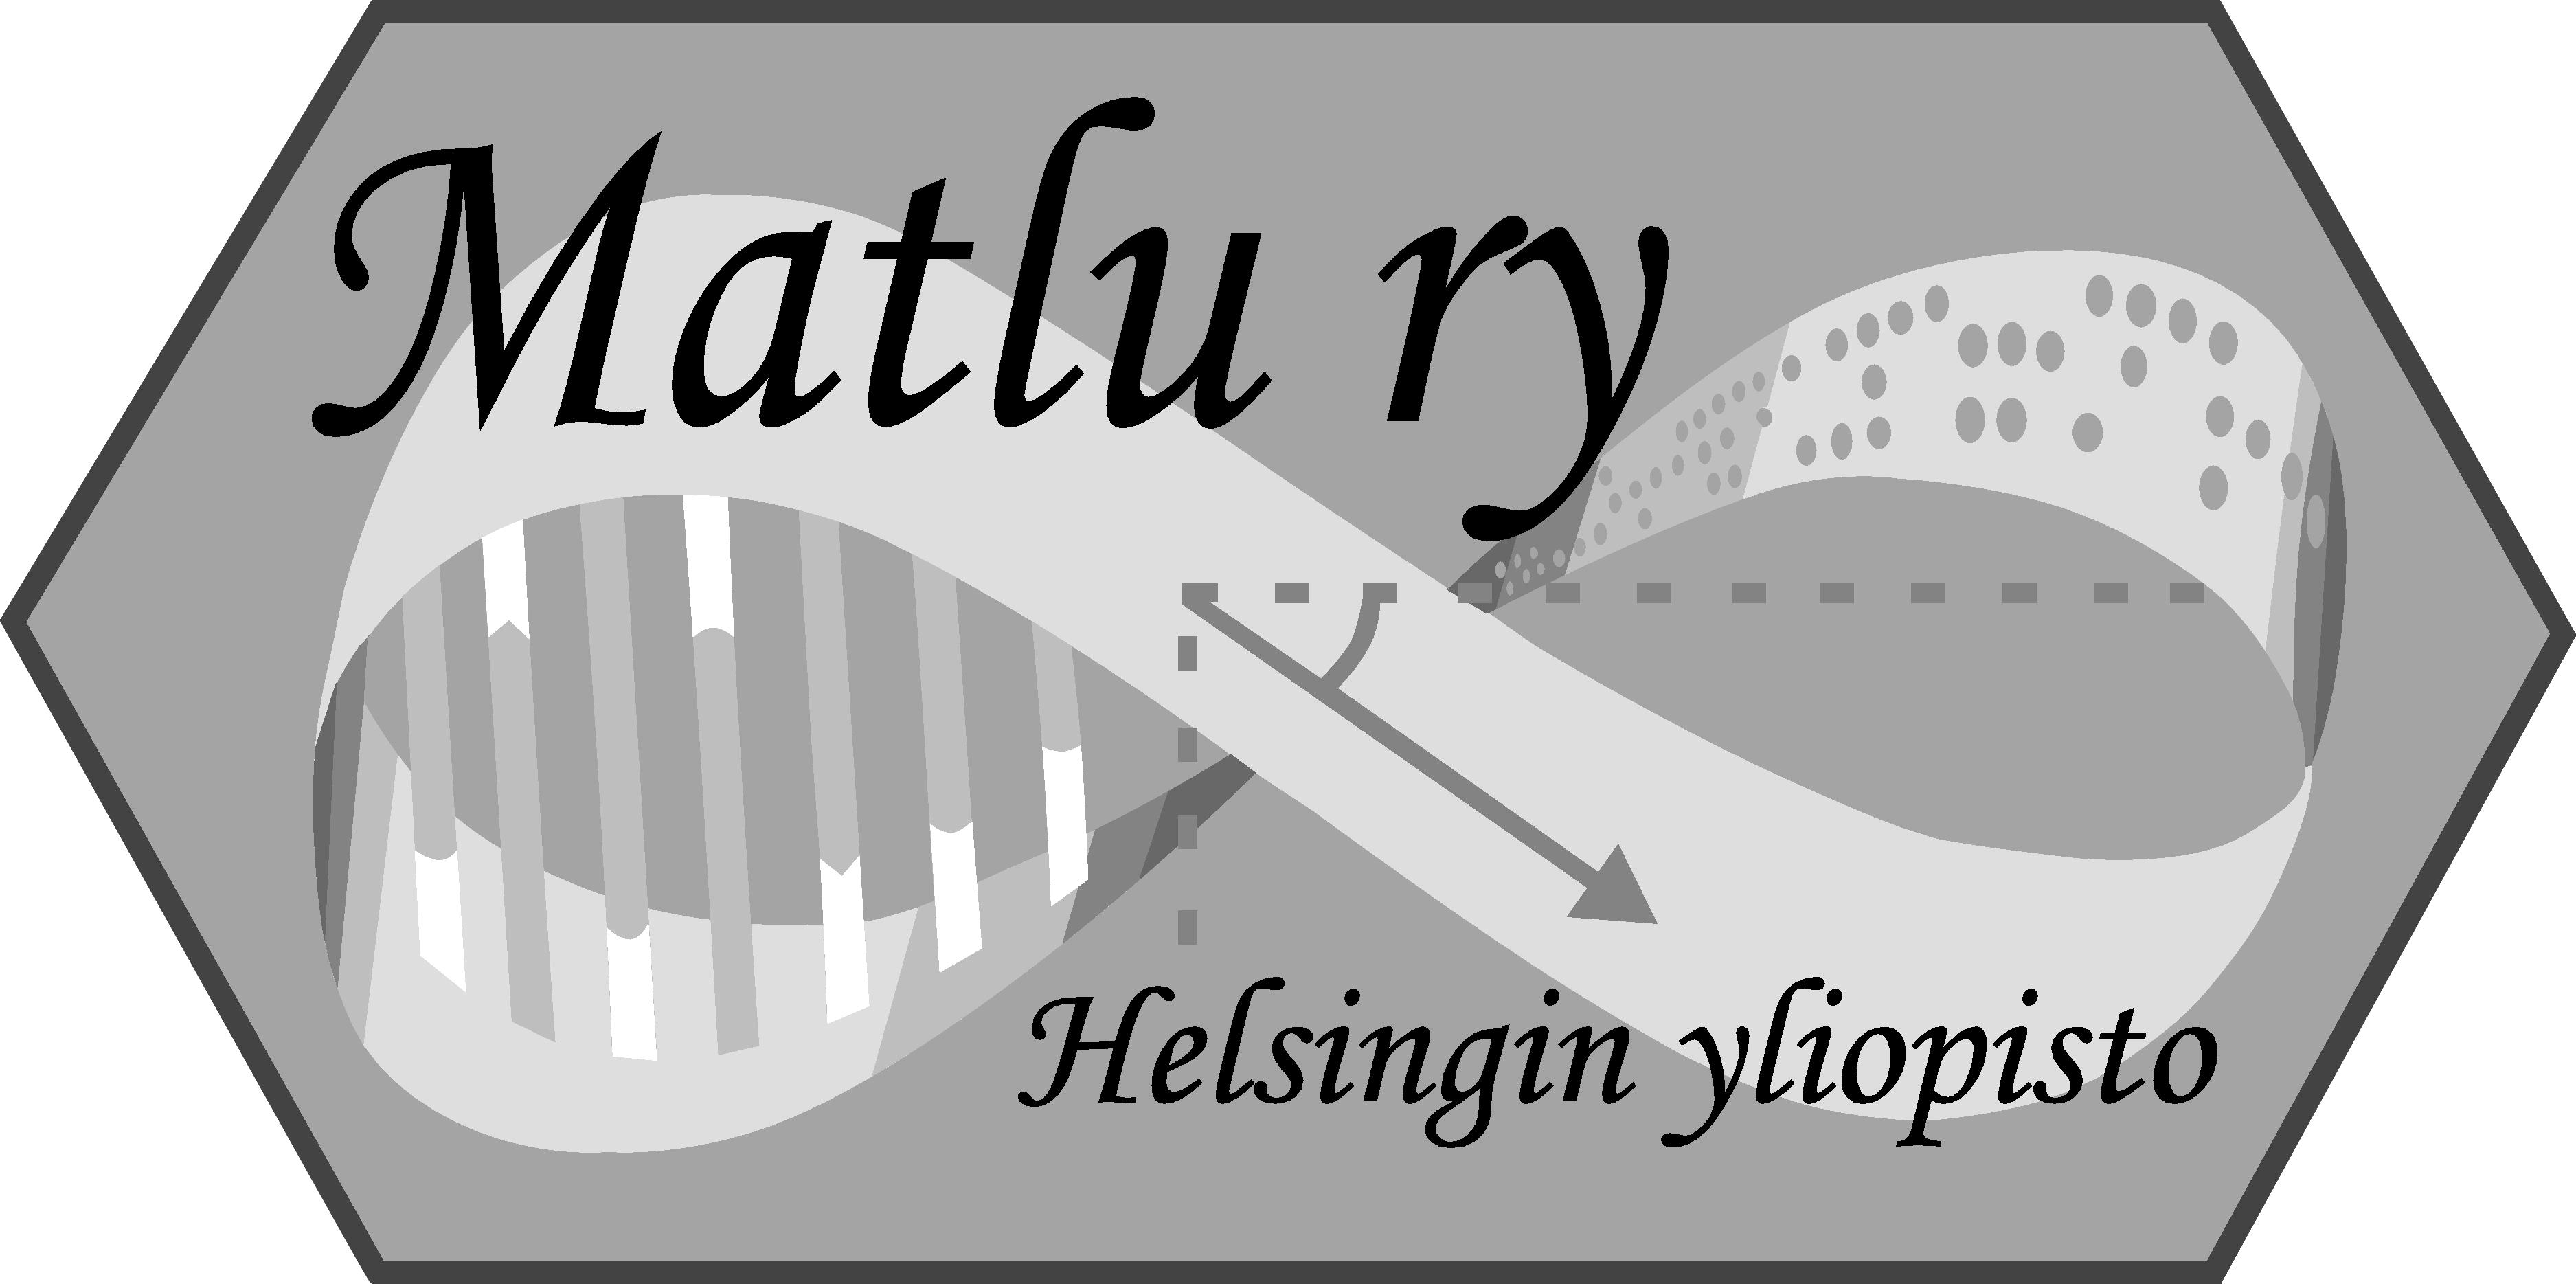
\includegraphics[width=\columnwidth]{matlu.png}
\end{figure}
Limesläisenä olet myös matlulainen,
sillä Matlu~ry on matemaattis-luonnon\-tieteellisten
opiskelija\-järjestöjen yhteis\-työ\-järjestö.
Siihen kuuluvat kaikki Kumpulan
aine\-järjestöt, ja Matlu on siten Kumpulan suurin yhteinen tekijä.
Suurena järjestönä Matlulla on mahdollisuus
toteuttaa opiskelijoiden laajempaa edunvalvontaa ja
järjestää massiivisempia tapahtumia
kuin yksittäisillä järjestöillä, joten
vain taivas on rajana.

Matlun toimenkuvat vaihtelevat tiedekuntatason
politikoinnista ja tuutoroinnin avustamisesta
bileiden, suunnistusten sekä työelämätapahtumien
järjestämiseen. Olet jo ehkä saattanut käydä Matlun lukuvuoden
ensimmäisissä bileissä, kesäbileissä. Syksyn tullen pääset
näkemään vielä fuksibileet, Halloween-bileet ja
lähtölaukauksen työelämään Kumpulan Potentiaalissa.

Matlun tapahtumat ovat mitä mainioin
tapa tutustua niihin muiden koulutusohjelmien kummajaisiin,
joita tulee silloin tällöin nähtyä
kampusten laajoilla aukioilla. Laajemmin
Matlun toimintaan voi tutustua kotisivuillamme
tai ottamalla yhteyttä Opetushallituksen
sijasta johonkin Matlun aktiiviin.
Matlun toiminta ja hallituksen kokoukset ovat
ainejärjestöjen tavoin avoimia kaikille, joten jos
kiinnostus toimintaan lähtemiseen heräsi, tervetuloa!

\noindent URL: \url{www.matlu.fi}

\noindent e-mail: \\\url{matlu-aktiivit@helsinki.fi}

\twocolumn[\section{Osakunnat}]
\subsection*{Mikä?}
Osakuntien juuret ovat kaukana, aina
1100-luvun Ranskassa. Alun perin oli
ajatuksena koota yhteen samalta seudulta
kotoisin olevia opiskelijoita, parantaa yhteyksiä
kotiseutuun ja tukea kaukana kotoaan
olevia opiskelijoita.

Osakunnat ovat olleet aina ja ennen
kaikkea osakuntalaisten yhdessäoloa: sivistynyttä keskustelua, nousu- ja laskuhumalaa,
pöytäjuhlia sekä hyvässä seurassa
valvottuja öitä. Perinteitäkin pidetään
yllä esimerkiksi tekemällä kotiseuturetkiä.
\subsection*{Ketä?}
Helsingin yliopiston osakunnissa on
yliopisto-opiskelijoita laidasta laitaan. Osakunnat
ovat niitä harvoja järjestöjä, joissa
on edustettuna niin matemaatikot, puutarhatieteilijät,
lääkärit kuin vaikka valtiotieteilijät.
Tuurilla bongaat myös muutamia
teekkareita ja ehkä jopa kylterin.
\subsection*{Mitä?}
Kaikilla osakunnalla on oma talo tai huoneisto, jossa jäsenet kokoontuvat harrastamaan, juhlimaan, organisoimaan toimintaansa ja ennen kaikkea viettämään aikaa yhdessä. Järjestettyjen tapahtumien ohella osakunnan luonteeseen kuuluu kodinomaisuus: jäsenet voivat viettää siellä vapaa-aikaansa, esimerkiksi lukea lehtiä, opiskella, käyttää nettiä, katsoa televisiota tai ihan vain hengailla. Lisäksi osakunnat tarjoavat halpoja asuntoja ja stipendejä jäsenilleen.

Vaikka voit kuulua vain yhteen osakuntaan, olet tervetullut vierailemaan kaikissa!

\subsection*{Osakunnat Helsingin yliopistossa}
\begin{itemize}
	\item Nylands nation (NN)
	\item Eteläsuomalainen osakunta (ESO)
	\item Savolainen osakunta (SavO )
	\item Karjalainen Osakunta (KO)
	\item Hämäläis-Osakunta (HO)
	\item Keskisuomalainen Osakunta (KSO)
	\item Kymenlaakson Osakunta (KyO )
	\item Åbo Nation (ÅN)
	\item Varsinaissuomalainen Osakunta (VSO)
	\item Satakuntalainen Osakunta (SatO )
	\item Wiipurilainen osakunta (WiO )
	\item Östra Finlands Nation (ÖFN)
	\item Etelä-Pohjalainen Osakunta (EPO)
	\item Vasa nation (VN)
	\item Pohjois-Pohjalainen Osakunta (PPO)
\end{itemize}

\noindent URL: \url{www.osakunta.fi}

\vspace{0.5cm}\noindent\textsc{Sakari Väkevä}
\chapter{Verkossa}
\twocolumn[\section{Tietotekniikkapalvelut}]
\begin{figure*}[!b]\fbox{\begin{minipage}{\textwidth}\centering
			Joka vuosi 10~000 uutta opiskelijaa
			saa käyttäjätunnuksen\\Lääkintöhallitus
\end{minipage}}\end{figure*}
\subsection*{Käyttöluvat}
Yliopiston tieto\-tekniikka\-palvelujen käyttämiseen
tarvitsee pää\-käyttö\-luvan eli AD-tunnuksen. Uudet
opiskelijat saavat sellaisen automaattisesti ottaessaan opiskelu\-paikan vastaan. Lisäksi tietojen\-käsittely\-tieteen opiskelijoiden on otettava käyttöön CS-tunnukset osoitteesta \url{https://www.cs.helsinki.fi/passwd}.

\subsection*{Windows-työasemat}
Physicumin kirjastossa on yliopiston Windows-koneita. Exactumissa on useita tieto\-kone\-luokkia.
Pohjakerroksesta löytyvät lisäksi 24h-luokat. Chemicumin mikroluokat löytyvät ensimmäisestä
kerroksesta.  Jokaisesta Kumpulan kampuksen rakennuksesta
löytyy ainakin yksi skannerilla
varustettu tieto\-kone\-luokka.

Keskustasta koneita löytyy Aleksandriasta
(Fabianinkatu~26) sekä kasvatus\-tieteellisen
tdk:n yhteydessä toimivalta
oppimiskeskus Minervalta Siltavuorenpenkereeltä.
Molemmista löytyy myös 24h-luokat.
Jo mainittujen 24h-tilojen lisäksi
myös Viikistä löytyy yksi 24h-luokka.

\subsection*{Kotihakemisto (Z-asema)}
Lähes kaikilta yliopiston koneilta pääsee käyttäjän omaan kotihakemistoon (Z-asemaan), jossa voi säilyttää omia tiedostojaan, ja johon
muut eivät pääse käsiksi. Z-asemalle on varattu 20~giga\-tavua säilytys\-tilaa, lisää löytyy OneDrivesta. Koska tiedostoja
säilytetään verkkolevyllä, käyttäjä pääsee
niihin käsiksi miltä tahansa yliopiston koneelta.

\subsection*{UNIX-koneet}
AD-tunnuksilla uusi opiskelija pääsee kirjautumaan UNIX-koneelle \url{pangolin.it.helsinki.fi}, jossa voi pyörittää irkkiä. Käpistelijöiden kannattaa kuitenkin käyttää TKT-osaston UNIXeja kuten melkkiä tai melkin\-paasia, joihin pääsee CS-tunnuksilla. UNIXeihin törmää joka
tapauksessa ennemmin tai myöhemmin,
joten kannattaa aloittaa tutustuminen ajoissa,
ettei mene sormi suuhun sitten kun niitä
todella tarvitsee.

UNIX-koneita käytetään ottamalla niihin
SSH-yhteys miltä tahansa nettiin kytketyltä
koneelta. Yhteyden ottamiseen tarvitaan SSH-ohjelma,
Windowsissa esimerkiksi Putty, muissa ympäristöissä usein komento \texttt{ssh} riittää. Tiedostojen siirto onnistuu
\texttt{scp}-ohjelmalla -- Windows-koneille näitä löytyy ainakin WinSCP, muissa ympäristöissä usein riittää komento \texttt{scp}. 

Putty- ja WinSCP "-ohjelmat ovat ilmaisia ja ne
voi käydä hakemassa kotikoneelle netistä
googlettamalla.

Lisäksi yli\-opistolta löytyy tilastollinen ja matemaattinen UNIX-palvelin \texttt{mutteri}, jolta löytyy
mm.\,Mathematica ja Matlab. Mutterin käyttö\-lupaa täytyy anoa erikseen, ks.\,\url{https://flamma.helsinki.fi/fi/HY053492}.

\subsection*{Magneettiavain, magneettia vain?}
24h-luokkiin on mahdollista saada magneettiavain,
jolla niihin pääse sisälle myös
iltaisin, öisin ja viikonloppuisin. Avaimen
hakeminen tapahtuu seuraavasti:

Tulosta ja täytä hakulomake, ja mene Gaudeamus kirja \& kahvi "-kahvilaan Kaisa-taloon. Kahvila tarkistaa lomakkeen, hakijan opiskelijakortin tai henkilökuntakortin, perii avainpantin (\EUR{25}) ja antaa avaimen.

Saat avaimen välittömästi ja se on käytettävissä
seuraavana päivänä.

\begin{figure}[!b]
	\centering
	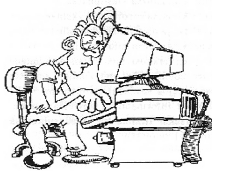
\includegraphics[width=\columnwidth]{ruuduntuijotus.png}
\end{figure}

\twocolumn[\section{Office365}]
Kun otat yliopiston tarjoaman Office365-paketin käyttöön, saat samalla Office-ohjelmistojen asennus\-oikeuden myös omille Windows- tai macOS-laitteille. Näihin kuuluvat mm.\,Microsoft Word, Excel, PowerPoint, Publisher ja muut vastaavat opiskeluissa hyödylliset työkalut.
\subsection*{Sähköposti}
Yliopiston tarjoamaan pilvi\-sähkö\-postiin kirjaudutaan osoitteessa \url{www.helsinki.fi/office365}. Yliopistolla edellytetään, että luet sähköpostiasi useamman kerran viikossa -- mielellään useamman kerran päivässä, sillä kaikki tiedotus tapahtuu lähtökohtaisesti sähköpostin välityksellä. Siksi sähköpostitilit kannattaa konffata myös omaan matkapuhelimeen, jolloin mikään viesti ei mene sinulta ohi päivän mittaan. Huomaa, että tällöin annat myös yliopiston Helpdeskille oikeuden etätyhjentää puhelimesi, mikäli se varastetaan tai dataa päätyy vääriin käsiin.

iOS-laitteilla sähköposti liitetään Mail-sovellukseen seuraavasti: Settings (Asetukset) $\rightarrow$ Mail, Contacts, Calendars (Posti, yhteystiedot, kalenterit) $\rightarrow$ Add Account (Lisää tili). Valitse tilin tyypiksi Exchange. Seuraa ohjeita. 

Huom! Palvelin = \url{outlook.office365.com}, domain = tyhjä, username = \texttt{adtunnus@ad.helsinki.fi}.

Android-laitteilla homma tapahtuu näin: Settings (Asetukset) $\rightarrow$ Accounts (Tilit) $\rightarrow$ Add account (Lisää tili) $\rightarrow$ Exchange. Seuraa ohjeita.
\subsection*{Kalenteri}
Pääset OWA-kalenteriin kirjautumalla sähköpostiisi nettiselaimella, painamalla vasemman yläkulman ruutu\-kuvaketta ja klikkaamalla Calendar (Kalenteri). Kalenterin kautta voit varata esimerkiksi kirjaston ryhmätyötiloja. Tämä onnistuu luomalla uuden tapahtuman (New event) ja klikkaamalla Add room (Lisää huone) "-painiketta.
\subsection*{OneDrive}
Yliopisto tarjoaa sinulle teratavun verran tallennustilaa dokumenttien ja tiedostojen jakamiseen. Jos olet esimerkiksi kirjoittamassa Wordilla raporttia kaveriesi kanssa, voit editoida sitä OneDrivessä useammalta koneelta yhtä aikaa. Voit tallentaa tiedostoja Office-ohjelmista suoraan OneDriveen, kunhan olet ensin kirjautunut sisään yliopiston tunnuksillasi.

Nettiselaimen kautta One\-Driveen pääsee Internet-osoitteesta \url{https://helsinkifi-my.sharepoint.com}. Syötä käyttäjätunnus muodossa \texttt{adtunnus@ad.helsinki.fi}.

Yli gigatavun kokoiset tiedostot kannattaa jakaa Funet FileSenderissä: \url{https://filesender.funet.fi/}.

\twocolumn[\section{Tulostaminen}]
Yliopistolla ei ole enää ilmaista opiskelija\-tulostusta, minkä vuoksi opiskelijalla on oikeus palauttaa kaikki opintoihin liittyvät tehtävät sähköisesti (ks.\,vara\-rehtorin päätös~11/2015). Mikäli et jaksa latoa laskareita siististi {\LaTeX}illa, Canon-monitoimilaitteita voi käyttää skannaamiseen.

Mikäli haluat printata jotain, eikä yliopistolla työsuhteessa oleva tuutorisi jaksa auttaa sinua, joudut hankkimaan tulostussaldoa. Saldoa saa Unigrafian verkkokaupasta (\url{https://tulostus.unigrafia.fi/tulostussaldo}). Tulostus\-tilille pitää ladata kerralla vähintään \EUR{5}. Mustavalko\-tulostus maksaa vajaat 7~snt/sivu ja väri\-tulostus reilut 20~snt/sivu.

Voit lähettää töitä tulostus\-jonoon yliopiston keskitetysti ylläpitämiltä koneilta valitsemalla printteriksi Smartcard-PCL- tai Smartcard-PS "-alkuisen nimen. Omalta koneelta voit lähettää valmiita PDF-tiedostoja tulostusjonoon käyttämällä verkko\-palvelua \url{https://wpr.helsinki.fi}. Voit noutaa työn miltä tahansa yliopiston Smartcard-printteriltä vilauttamalla sille matkakorttiasi. Ensimmäisellä tulostuskerralla printteri kysyy myös AD-tunnustasi ja salasanaa.
\begin{figure}[b!]
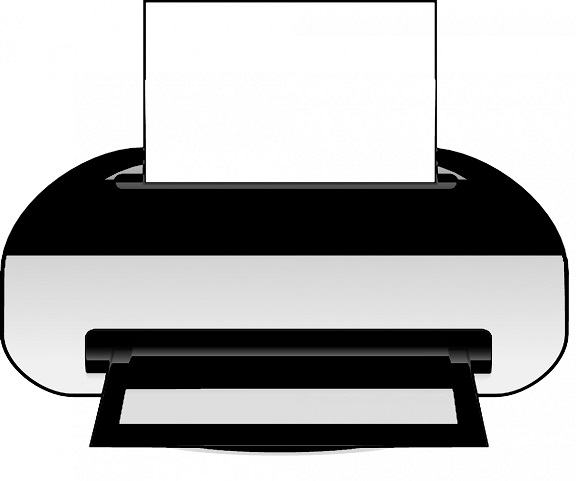
\includegraphics[width=0.9\columnwidth]{computer-printer.jpg}
\end{figure}
\twocolumn[\section{Opiskelijan tietojärjestelmät}]
\subsection*{Oili}
OILI on korkeakoulujen opiskelijaksi- ja lukukausi-ilmoittautumispalvelu, jossa korkeakoulujen yhteishaussa opiskelupaikan saanut opiskelija voi sähköisesti ilmoittautua opiskelijaksi korkeakouluun sekä tarvittaessa maksaa esim. ylioppilaskunnan jäsenmaksun.\,Korkeakoulu voi hyödyntää OILIa myös jatkavien opiskelijoiden ilmoittautumisten vastaanottamiseen.

\noindent URL: \url{https://oili.csc.fi}

\subsection*{WebOodi}
WebOodi on opiskelijoiden käyttöön
kehitetty verkkopohjainen opiskelija- ja
suoritustietojärjestelmä. WebOodia pääsee
käyttämään voimassaolevilla yliopiston
mikroverkkotunnuksilla.

Weboodissa voit:
\begin{itemize}
	\item Muuttaa yhteystietojasi (Postiin ja Väestö\-rekisteri\-keskukseen
	tehdyt osoitteenmuutokset eivät välity yliopistolle!)
	\item Tilata epävirallisen opinto\-suoritus\-otteen
	\item Seurata suoritustesi rekisteröitymistä
	\item Tehdä luku\-kausi-ilmoit\-tautu\-misen
	\item Ilmoittautua tentteihin ja opetukseen
\end{itemize}
Nykyään opetukseen ja tentteihin ilmoittautuminen
tehdään käytännössä kokonaan
WebOodissa, mutta ilmoittautumiskäytännöt
vaihtelevat välillä kurssista riippuen.
TKT:n ilmoittautumiset hoituvat
omasta ilmo-järjestelmästä. Myös luonnontieteellisessä tiedekunnassa
on ainakin keskustelu tasolla ollut
pyrkimyksenä siirtää kaikki informaatio
kursseista ja ilmoittautumiset WebOodiin.
Pikku hiljaa ne sinne tuntuvat sinne menevänkin.
Myös henkilökohtaisen opintosuunnitelman
Hopsin tekeminen on siirtymässä
WebOodiin.

\noindent URL: \url{https://weboodi.helsinki.fi}

\subsection*{Opiskelijan ohjeet}
Opiskelijan ohjeet kokoaa yliopiston yhteiset ja koulutusohjelmakohtaiset ohjeet ja muut neuvonta-aineistot yhteen paikkaan, jotta ne muodostavat opiskelijalle käytettävän ja loogisen kokonaisuuden.

Valitse koulutusohjelmasi, jotta saat näkyviin kaikki opintoihisi liittyvät ohjeet. Ohjeet on jaoteltu teemoihin, jotka löydät sivua alaspäin selaamalla. Ohjeita voit hakea myös sanahaulla. Sisällöt täydentyvät vielä, joten jos et löydä etsimääsi, ota yhteys opiskelijaneuvontaan.

Opiskelijan ohjeet koskevat pääosin 1.8.2017 aloittaneita koulutusohjelmia, mutta osa ohjeistuksesta on kaikille opiskelijoille yhteistä. Vanhan koulutusrakenteen mukaista ohjeistusta löytyy edelleen Flammasta.

\noindent URL: \url{https://student.helsinki.fi}
\subsection*{Moodle}
Moodle on ns.\,verkko-oppimis\-ympäristö, jota voidaan käyttää esimerkiksi kurssin ilmoitustauluna, opetusmateriaalien jakamiseen, verkkokeskustelemiseen, tenttimiseen tai oppimistehtävien/tiedostojen palautukseen.

\noindent URL: \url{https://moodle.helsinki.fi}
\subsection*{SISu}
Älä käytä, ennen kuin tämä saadaan oikeasti toimimaan.

\subsection*{Miten pääsen nettiin?}
\subsubsection*{HUPnet}
\begin{figure}[h!]
	\centering
	
\includegraphics[width=\columnwidth]{hupnet.png}
\end{figure}
Helsinki University Public Network
(HUPnet) on verkko, johon käyttäjätunnuksen
omistava yliopistolainen voi kytkeytyä
omalla (kannettavalla) tietokoneellaan.
Mitään erityisiä ohjelmistoja ei tarvitse
asentaa. Yhteys Internetiin ja yliopiston
verkkoon aukaistaan www-selaimella autentikoimalla.
HUPnetiin voi kytkeytyä langattomasti
WLAN-verkkokortilla tai perinteisellä
Ethernet-verkkokortilla.

\subsubsection*{Eduroam}
\begin{figure}[h!]
	\centering
	
\includegraphics[width=\columnwidth]{eduroam_logo.png}
\end{figure}
Eduroam on suojattu langaton verkko, ja siksi sen käyttöä suositellaan. Eduroam on valmiiksi asennettuna yliopiston keskitetysti hallituilla koneilla. Omille koneille Eduroam on asennettava itse. Eduroam-yhteyttä tarjotaan automaattisesti, kun olet sellaisessa tilassa, jossa on Eduroam-verkko.

Eduroamiin kirjaudutaan yliopiston käyttäjätunnuksella, joka kirjoitetaan muodossa \url{tunnus@helsinki.fi}. Muiden korkeakoulujen vierailijat voivat kirjautua Eduroamiin oman kotiorganisaationsa käyttäjätunnuksilla, mikäli kyseinen organisaatio on osa Eduroam-verkostoa.

\twocolumn[\section{IRC} {\small \itshape ``<@Zirona> Uusi addiktoiva harrastus: IRKKAUS''}\vspace{0.5cm}]
Tuntuuko sinusta siltä, että elämästäsi
puuttuu jotain? Onko sinulla ollut jokin
hassu tunne, että kaikki ei ole sitä, miltä se
näyttää? Oletko aina halunnut mätkiä kavereitasi
Asterixmaisesti isolla taimenella?
Entäs tunnetko outoa kiihotusta tuijottaessasi
keskellä yötä tietokoneruutua, jossa vilisee
hämärää kirjoitusta? Havaitsiko aivosi
liikaa kysymyksiä, joihin et osaa vastata?
\begin{figure}[!b]
	\centering
	
\includegraphics[width=0.8\columnwidth]{irckuva.png}
\end{figure}

\texttt{/join \#limes}.

\texttt{\#limes} on Limes~ry:n virallinen (tai välillä
jutun tasosta päätellen ei niin virallinen)
IrcNetissä sijaitseva IRC-kanava eli
Internet Relay Chat. Kanavalle ovat tervetulleita
kaikki uudet ja jo rupsahtaneetkin
limesläiset. Jutun tasosta emme vastaa,
mutta asiaakin saattaa löytyä aina aika
ajoin (lue: vahinkoja sattuu).

Nyt sinun ei tarvitse enää nauraa yksiksesi
kotona. Voit nauraa kavereiden kanssa
yhtä aikaa ollessasi yksin kotona. Eikä
siinä vielä kaikki. Lisäksi voit harjoittaa
yhdessä muiden kanssa huonojen juttujen
kertomista, lollottelua, pomottelua ja jos
olet todella rohkea, voit jopa yrittää kirjoittaa
privaattiviestejä. Tunteitakin on lupa
näyttää erilaisten hymiöiden välityksellä,
jos sellaisia omistat\dots xD

Kaikista uskaliaimmat ovat jo tunnustautuneet
julkisesti irkkaajiksi ja löytyvät
\url{https://irc-galleria.net/} "-sivuilta. Uskallatko
katsoa kenen poskelle läimäyttelit suunnatonta
löysää pamppua? Houkutteleeko?
Joko säikähdit?

Irkkaamiseen pääsee erittäin helposti
mukaan. Tarvitset vain tietokoneen vuodelta
miekka ja kirves, nettiyhteyden sekä IRC-asiakas\-ohjelman
kuten irssin tai Mircin. Asettamalla
sopivat asetukset mm.\,ircserverin (esim.
\url{irc.cs.hut.fi}) ja oman hienon lempinimen
pääset liittymään \texttt{\#limes}-kanavalle. ``Ei
se oo kovin vaikiaa, kuha sen vaa oppii'',
sano isäntä, kun setoria ojahan ohojas. Lisää
perustietoutta irkistä löytyy osoitteesta:
\url{https://fuksiwiki.tko-aly.fi/IRC-ohjeet}.

\vspace{0.5cm}\noindent\textsc{Sanna Hautala}\footnote{Zirona lopettaa hörisemisensä tähän. Lisää tarjolla \texttt{\#limes}-kanavalla.}

\twocolumn[\section{Jodel}]
Jodel on mobiili\-viestintä\-sovellus, jonka käyttäjäkunta koostui alussa lähinnä korkea\-koulu\-opiskelijoista, mutta nykyään muutkin ikäryhmät ovat sen löytäneet. Sovellus antaa käyttäjien lähettää anonyymisti viestejä, jotka näkyvät 10~kilometrin säteellä oleville käyttäjille (``jodlauksia''). Viestin voi myös nähdä, jos on valinnut kyseisen kaupungin kotikunnakseen. Kotikuntia voi olla vain yksi, ja sen voi vaihtaa vain kerran.

Viesti voi olla valokuva tai 230~merkin pituinen teksti. Kuvia ei voi ladata kännykästä Jodeliin, vaan jokainen kuva täytyy ottaa kameralla sovelluksen kautta. Kuvan päälle saa luotua lyhyen kuvatekstin tai piirrettyä.

Jokaista Jodeliin lähetettyä viestiä voi kommentoida sekä äänestää ylös tai alas. Viestin saamat kokonais\-äänet näkyvät viestin oikeassa laidassa. Jodlauksen tekijä voi yläpeukun lisäksi kiittää vastaajaa, jolloin vastauksen äänien yläpuolelle ilmestyy sydän. Viesti poistuu, jos sen saamien äänien summa on miinus viisi tai alempi. Asiattomia viestejä voi myös liputtaa, jolloin moderaattorit tarkastavat viestin sisällön.

Avatessasi Jodelin päädyt mainfeedille, jossa keskustellaan kaikesta yleisesti. Mainfeedin lisäksi on eri kanavia, joilla keskustelu rajoittuu tiettyyn aihepiiriin. Esim.\,\texttt{@kissa}-kanavalle ihmiset lähettävät kuvia kissoistaan, ja \texttt{@patonki}-kanavalla voi tiedustella, mitä patonkeja Physicumin kahvilassa on tänään tarjolla. Kanavia voi etsiä Kanavat "-välilehdellä olevaa suurennuslasia painamalla. Toinen vaihtoehto on kirjoittaa jodlaukseen tai vastaukseen \texttt{@halutunKanavanNimi}, jolloin kanavalle pääsee viestiä klikkaamalla.  

Jokaisella jodlaajalla on karma. Karmaa kertyy, kun jodlaukset ja vastaukset saavat ylä-ääniä, ja vähenee, jos saat tai annat alaääniä. Karma on erään\-lainen mittari, joka kertoo, kuinka aktiivinen ja suosittu olet Jodelissa. Se ei näy muille käyttäjille, eikä sillä oikein tee mitään. Ainoa etu on, että 20~000~karma\-pisteellä ja hyvällä käytöksellä (ei suurta määrää miinus\-ääniä saaneita viestejä) pääsee moderaattoriksi.

Kanavasuosituksia:
\begin{itemize}
	\item @helsinginyliopisto
	\item @kumpulankampus
	\item @matluihastus
	\item @patonki/@salaatti/@keitto
\end{itemize}

\vspace{0.5cm}
\noindent\textsc{Auli Salmi}

\twocolumn[\section{IRC ja Jodel -- jotain suosittuja lyhenteitä}]
\begin{table}[h!]
	\begin{tabularx}{\textwidth}{lX}
		AF &= as f*ck, todella, erittäin \\
		AFAIK &= as far as I know, tietääkseni \\
		AP &= aloituspostaaja, se joka aloitti keskustelun jostain aiheesta \\
		ASAP &= as soon as possible, pronto pronto \\
		BAE &= before anyone else, oma rakas \\
		BRB &= be right back, käväisen sioilla \\
		BTW &= by the way, asiasta kuudenteen \\
		CU &= see you! moikka! \\
		FYI &= for your information, tiedoksesi \\
		HTH &= hope this helps, koeta nyt suoriutua \\
		HAND &= have a nice day, hauskaa päivänjatkoa \\
		IIRC &= if I recall correctly, tai jotain \\
		IMHO &= in my humble opinion, vain minun vaatimaton mielipiteeni \\
		K &= key, okei \\
		LOL &= laughing out loud, kirjoittaja on jokseenkin huvittunut jostain \\
		MP &= mielipide, mitä jengi ajattelee tästä? \\
		OJ &= original jodler, sama kuin AP \\
		PLZ &= please, pliiiis \\
		ROTFL &= rolling on the floor laughing, kirjoittaja on erittäin huvittunut jostakin\\
		RSN &= real soon now, odota nyt hetki! \\
		RTFM &= read the fu**ing manual, jos vaivautuisit lukemaan ensteks sen käyttöohjeen, niin ei tarvis kysellä tyhmiä! \\
		T: Kari &= terveisin teekkari \\
		TTYL &= talk to you later, palataan astialle \\
		U/M &= uhka vai mahdollisuus?
	\end{tabularx}
\end{table}

\twocolumn[\section{Niksi-Pirkka tietokoneneroille}]
\begin{figure}[!b]
	\centering
	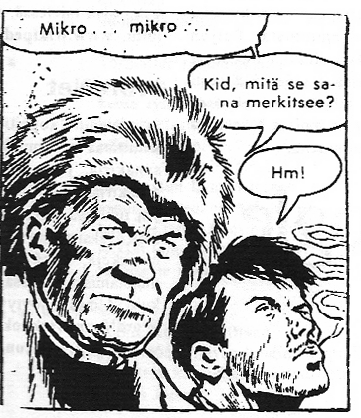
\includegraphics[width=\columnwidth]{mikroverkko.png}
\end{figure}
Mikroverkossa oleviin tiedostoihin pääsee
käsiksi mikroverkon ulkopuolelta osoitteesta:
\url{www.vpn.helsinki.fi}

Sähköpostilistoille liittyminen onnistuu
Majordomo-järjestelmän avulla. Ohjeet sen
käyttöön löytyvät Limeksen kotisivuilta
(\url{www.limes.fi}) kohdasta Tiedotus \textgreater Postituslista.

Yliopistolla opiskelevien ja työskentelevien
sähköpostiosoitteet voi etsiä kätevästi
mainarilla: \url{www.helsinki.fi/mainari}.

Yliopiston opiskelijoille lisensoimia
ohjelmia saa ladattua osoitteesta: \url{https://ohjelmistojakelu.helsinki.fi}.
Lisäksi myös Office Pro Plus "-paketin ohjelmat ovat yliopiston opiskelijoille ilmaisia.

Oman kotisivun tekemiseen ja julkaisemiseen
yliopiston palvelimella löytyvät
ohjeet osoitteesta \url{https://helpdesk.it.helsinki.fi/help/3078}.

Helsingin yliopiston materiaalipankki tarjoaa yliopiston esittelymateriaalia, posteri- ja diaesityspohjia sekä logoja. Se löytyy osoitteesta \url{https://unimaterialbank.unigrafia.fi}.

Vain yliopiston koneilta toimivia elektronisia
lehtiä, tietokantoja ja muita verkkopalveluita
pääsee käyttämään omalta kotikoneelta
asentamalla VPN-ohjelmiston,
joka saa kotikoneen näyttämään yliopiston
verkossa olevalta koneelta. \url{https://helpdesk.it.helsinki.fi/help/5190}.

\begin{figure}[!b]
	\centering
	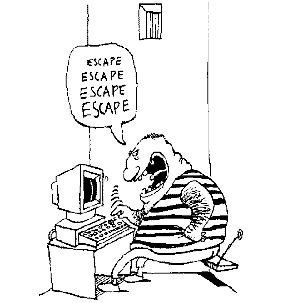
\includegraphics[width=\columnwidth]{escnappi.png}
\end{figure}

UNIXissa irkkaaminen onnistuu Pangolin-palvelimelta
löytyvällä irssi-ohjelmalla,
jonka hakemistopolku on: 

\noindent\texttt{/usr/bin/irssi}

Ensin kannattaa kuitenkin ajaa komento \texttt{screen -R irssi}. Komento luo virtuaalisen terminaalin, jonka sisällä voit käynnistää irssin. Terminaali menee piiloon näppäinyhdistelmällä Ctrl--A, Ctrl--D ja palaa, kun kirjoitat \\\texttt{screen -dr}. Virtuaalisen terminaalin avulla IRC-ohjelmasi pysyy jatkuvasti päällä, vaikka SSH-yhteys katkeaisikin välissä. Näin et missaa yhtään saapuvaa viestiä. Tieto\-tekniikka\-keskus tosin ei erityisemmin tykkää tästä!

Jos UNIX-istuntosi on mennyt salaperäisesti
jumiin, varmista ettet ole vahingossa
pysäyttänyt näyttöä näppäilemällä
Ctrl--S. Koeta vapauttaa näyttö näppäilemällä
Ctrl--Q. Jos mitään ei tapahdu, syy
on muualla.

\twocolumn[\section{Yliopiston hierarkia}]
\begin{table}[h!]
	\begin{tabularx}{\textwidth}{lX}
\textbf{Kansleri} &= Ylittää kerrostalon yhdellä ponkaisulla, on vahvempi kuin höyryveturi, nopeampi kuin kiitävä luoti, kävelee vetten päällä, keskustelee jumalan kanssa.\\
\textbf{Rehtori} &= Ylittää rivitalon yhdellä ponkaisulla, on vahvempi kuin yskivä veturi, yhtä nopea kuin kiitävä luoti, kävelee vetten päällä -- jos on tyyntä, puhuu jumalalle.\\
\textbf{Professori} &= Loikkaa yli omakotitalon juoksuvauhdilla myötätuulessa, on melkein yskivän veturin veroinen, hitaampi kuin kiitävä luoti, kävelee vetten päällä uima-altaassa, puhuu jumalalle, jos saa audienssin.\\
\textbf{Dosentti} &= Harvoin selvittää telttaa kummempaa, häviää junalle, osaa lähettää kiitävän luodin, ui hyvin, kuulee joskus jumalan äänen.\\
\textbf{Assistentti} &= Jättää jäljen seinään, jää junan alle, onnistuu joskus käyttämään asetta loukkaantumatta, ui koiraa, puhuu eläimille.\\
\textbf{Opiskelija} &= Törmäilee rakennuksiin, tunnistaa junan kaksi kertaa kolmesta, kerää tyhjät hylsyt, kelluu pelastusliiveillä, puhuu seinille.\\
\textbf{Fuksi} &= Kompastuu kynnykseen, sanoo ``Katsokaa, tuh-tuh'', kastelee itsensä vesipyssyllä, leikkii lammikossa, jokeltelee itsekseen. \\
\textbf{Osaston johtaja} &= Siirtää vuoria, potkii junia raiteiltaan, pyydystää kiitävän luodin hampaillaan ja syö sen, jäädyttää katseellaan valtameren, hän on Jumala.
	\end{tabularx}
\end{table}
\chapter{Opiskelijan sanasto}
\clearpage 
\subfile{sections/sanasto}
\twocolumn[\section{Limeksen jäseneksi liittyminen}
\noindent{\Large MIKSI}
\begin{itemize}
\item Saat alennuksia Limeksen bileistä, kirjoista jne.
\item Saat tiedon kaikista tulevista tapahtumista pääsemällä listalle
\item Saat olla kumpulalainen
\end{itemize}
\noindent{\Large MITEN}
\begin{itemize}
\item Täyttämällä joko elektronisen tai paperisen jäsenlomakkeen.
\item Maksamalla 2 euroa jäsenmaksua
\end{itemize}
\noindent{\Large MISSÄ}
\begin{itemize}
\item Osoitteessa \url{https://limes.fi/jasenyys/} (maksu tilille)
\item Orientoivissa, myynneissä, avajaiskarnevaaleilla ja järjestötorilla
\item Limeksen toimistolla (Exactum, huone~C132) aukioloaikoina
\end{itemize}{
\centering
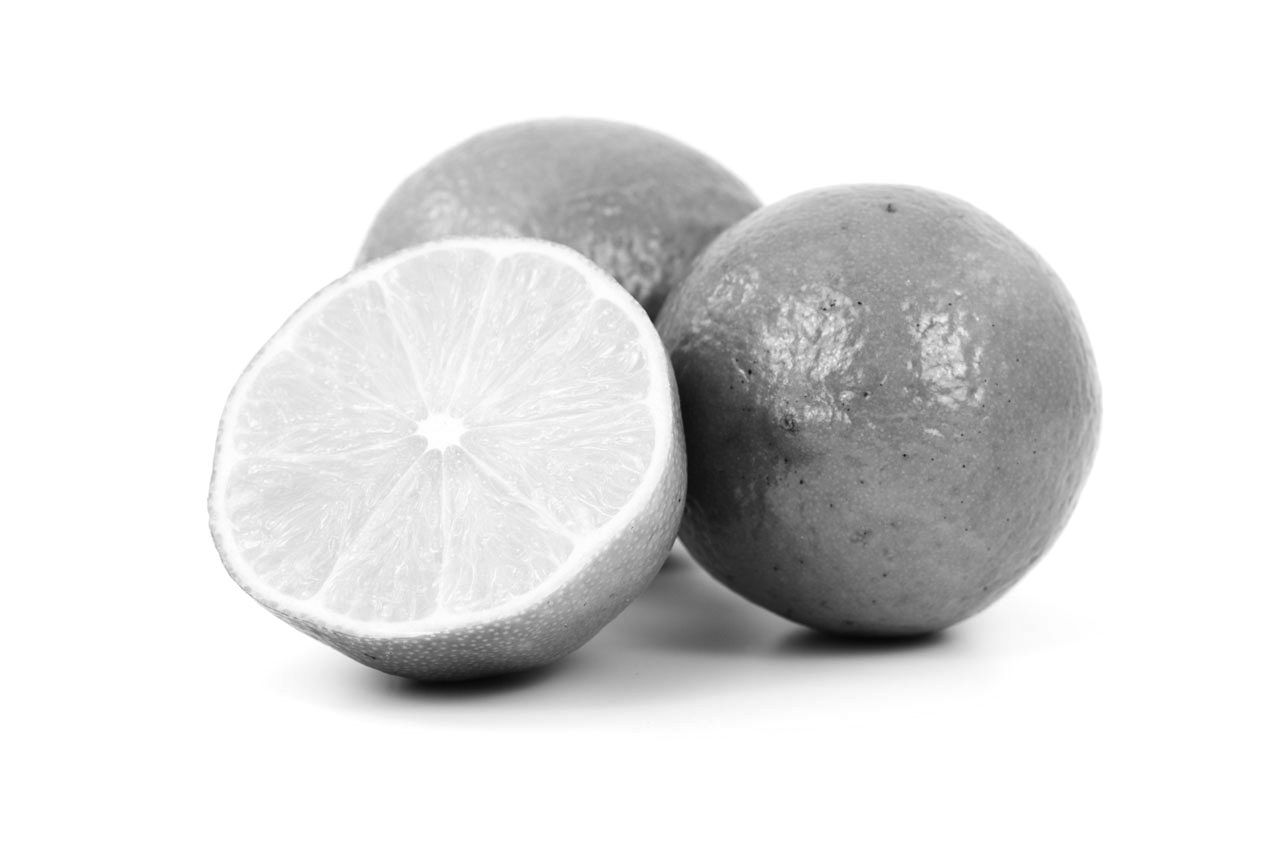
\includegraphics[width=\textwidth]{limes.jpg}
}]

\twocolumn[\section{Syksyllä tapahtuu!}
Osallistumalla Limeksen toimintaan pääset mukaan esimerkiksi näihin riemastuttaviin
aktiviteetteihin. $\varheart$

\vspace{2cm}
{
\centering
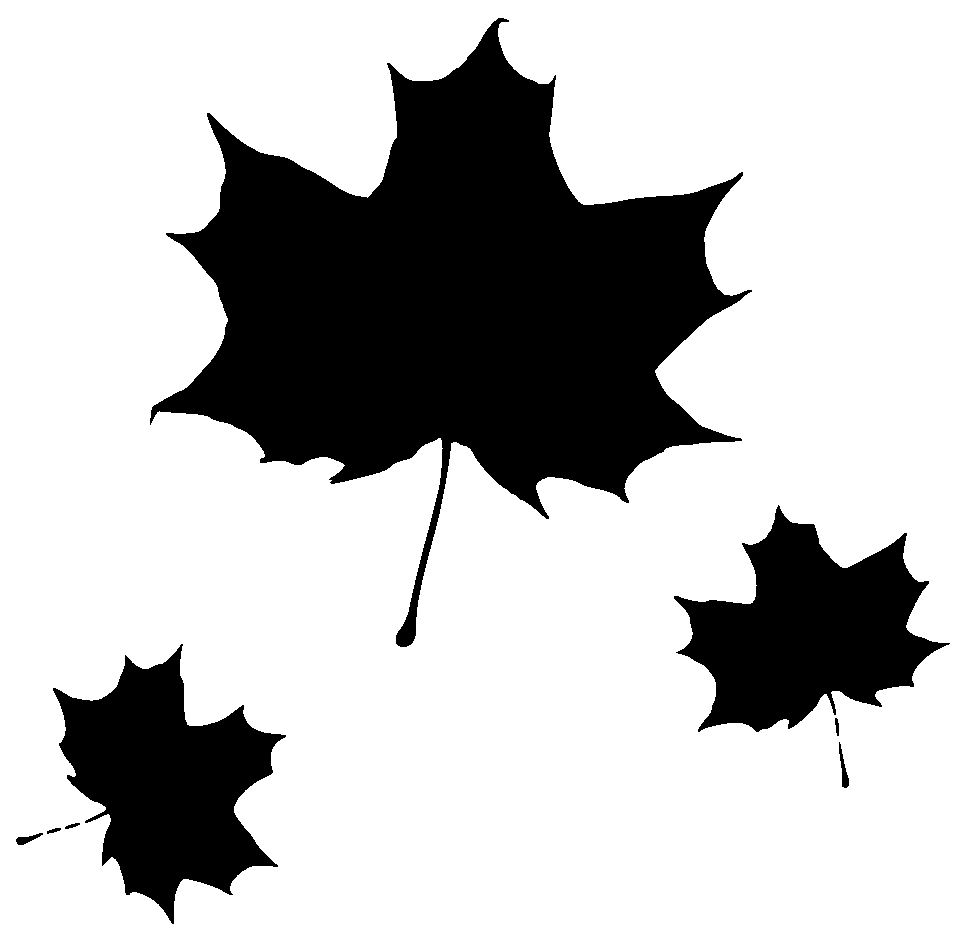
\includegraphics[width=0.8\textwidth]{vaahteranlehdet.eps}
}
\vspace{1cm}

\begin{tabularx}{\textwidth}{lX}
	25.--26.8. & Kumpulan fuksileiri (Rismalahti) \\
	31.8. klo 10--12 & Kumpulan koulutustarjonta "-info (Exactum A111) \\3.9. klo 21-- & Ex Tempore "-bileet, Kaivohuone\\
	20.9. & Limeksen Fuksisitsit\\
	3.10. & Limeksen Appro\\
	3.--5.11. & Kumpulan Järjestöjen YhteisRisteily (KJYR)
\end{tabularx}]
\cleartooddpage[]
\begin{figure*}[h!]
	\href{http://osakunta.fi/}{\includegraphics*[width=\textwidth]{osakunnat.png}}
\end{figure*}
\pagestyle{empty}
\begin{figure*}[h!]
\href{https://www.facebook.com/events/200128850801229/}{\includegraphics*[width=\textwidth]{fuksiseikkailu.jpg}}
\end{figure*}
\cleartoevenpage[]
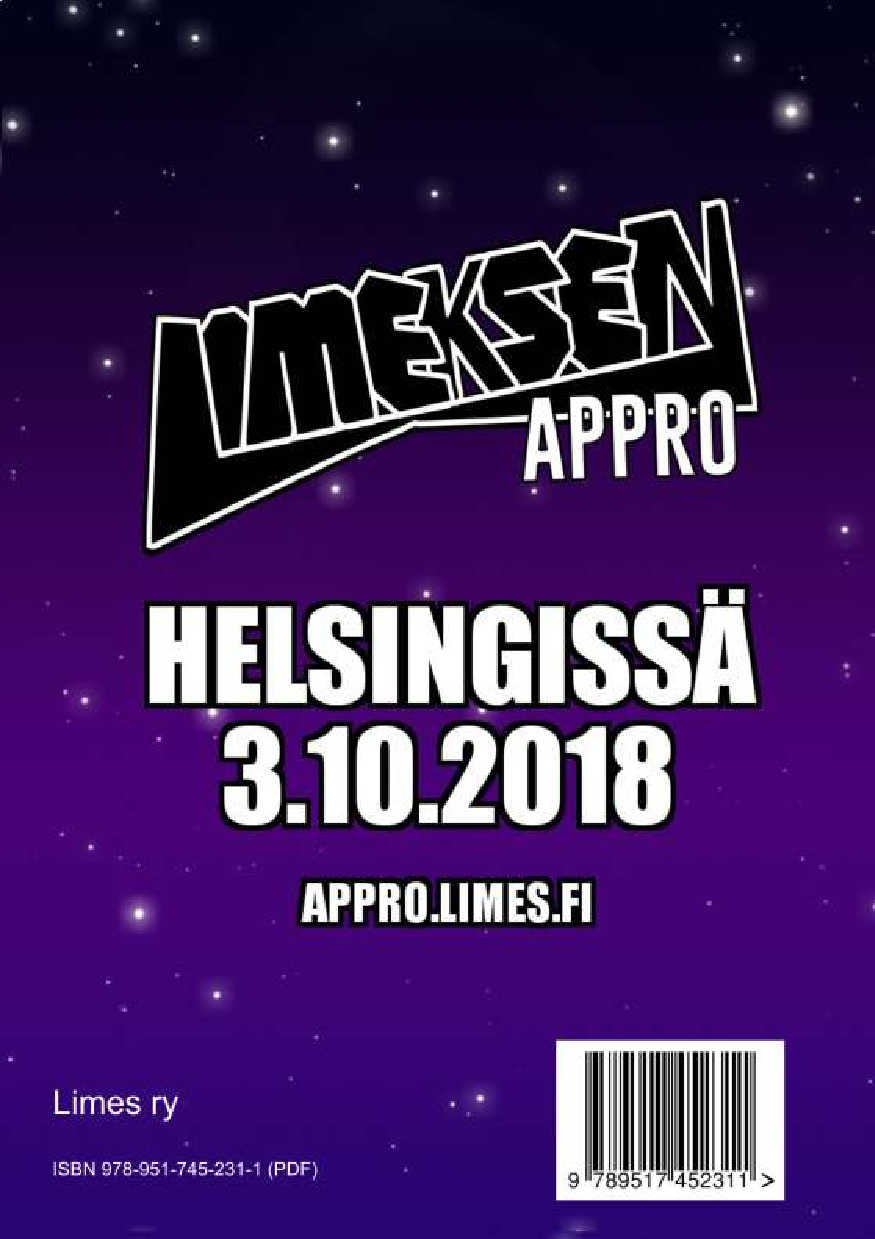
\includepdf[pages={-},angle=0]{ahistakakansi_digi.pdf}
\end{document}